\documentclass[]{fairmeta}

\usepackage{amsmath,amsthm,amssymb,bm}
\usepackage{color}
\usepackage{algorithm}
\usepackage[noend]{algpseudocode}
\usepackage[ruled,algo2e]{algorithm2e}%
\usepackage{derivative}
\usepackage{longtable}
\usepackage{pifont}
\usepackage{mdframed}
\usepackage{enumitem}
\usepackage{mathrsfs}
\usepackage{nicefrac}
\usepackage{subcaption}
\usepackage{float}
\newfloat{algorithm}{t}{lop}

\usepackage[normalem]{ulem}

\usepackage{siunitx}
\usepackage{tocloft}

\let\oldaddcontentsline\addcontentsline
\newcommand{\stoptocentries}{\renewcommand{\addcontentsline}[3]{}}
\newcommand{\starttocentries}{\let\addcontentsline\oldaddcontentsline}

\usepackage{tikz}
\usetikzlibrary{positioning, fit, calc}

\usepackage{booktabs}

\usepackage{arydshln} % Required for dashed lines

%
% --- inline annotations
%
\newcommand{\red}[1]{{\color{red}#1}}
\newcommand{\todo}[1]{{\color{red}#1}}
\newcommand{\TODO}[1]{\textbf{\color{red}[TODO: #1]}}
% --- disable by uncommenting  
% \renewcommand{\TODO}[1]{}
% \renewcommand{\todo}[1]{#1}

\usepackage{xcolor}
\usepackage{graphicx}
\usepackage{booktabs}
\usepackage{amsmath} 
\usepackage{amsfonts}
\usepackage{amssymb}
\usepackage{multirow} 
\usepackage{makecell}
\newcommand{\shline}{\Xhline{1.1pt}} % Adjust thickness as desired

% Shorthands for this project
\newcommand{\fX}{\bm{X}}
\usepackage{xspace}
\newcommand*{\eg}{{\it e.g.}\@\xspace}
\newcommand*{\ie}{{\it i.e.}\@\xspace}
\DeclarePairedDelimiterX{\infdivx}[2]{(}{)}{%
  #1\;\delimsize\|\;#2%
}
\newcommand{\infdiv}{D_\text{KL}\infdivx}
\newcommand*{\matr}[1]{\mathbfit{#1}}
\newcommand*{\tran}{^{\mkern-1.5mu\mathsf{T}}}

\definecolor{mygray}{gray}{0.95}
\newcommand{\graybox}[1]{%
\vspace{-1em} 
\begin{center}			% Centering minipage
\colorbox{mygray} {		% Set's the color of minipage
\begin{minipage}{0.987\linewidth} 	% Starts minipage
\centering
\vspace{-1em}   
{#1}    
\end{minipage}}			% End minipage
\end{center}
}

% \theoremstyle{definition}
% \newtheorem{definition}{Definition}[section]

\title{Adjoint Matching: Fine-tuning Flow and Diffusion Generative Models with Memoryless Stochastic Optimal Control}

\author[1]{Carles Domingo-Enrich}
\author[1]{Michal Drozdzal}
\author[1]{Brian Karrer}
\author[1]{Ricky T. Q. Chen}
\affiliation[1]{FAIR, Meta}

\abstract{
    Dynamical generative models that produce samples through an iterative process, such as Flow Matching and denoising diffusion models, have seen widespread use, but there have not been many theoretically-sound methods for improving these models with reward fine-tuning.
    In this work, we cast reward fine-tuning as stochastic optimal control (SOC). 
    Critically, we prove that a very specific \emph{memoryless} noise schedule must be enforced during fine-tuning, in order to account for the dependency between the noise variable and the generated samples.
    We also propose a new algorithm named \emph{Adjoint Matching} which outperforms existing SOC algorithms, by casting SOC problems as a regression problem. 
    We find that our approach significantly improves over existing methods for reward fine-tuning, achieving better consistency, realism, and generalization to unseen human preference reward models, while retaining sample diversity.
}

\stoptocentries

% \date{\today}
\correspondence{Carles Domingo-Enrich at \email{cd2754@nyu.edu}}

% \metadata[Code]{\url{TBD}}

\begin{document}

\maketitle

\section{Introduction}
\label{sec:intro}

\begin{figure}[b!]
    \vspace{-1.5em}
    \centering
    \begin{subfigure}[t]{0.495\linewidth}
        \centering
        \caption*{Base model (Flow Matching) w/ Guidance}
        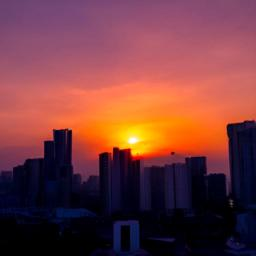
\includegraphics[width=0.32\linewidth]{figs/samples/cfg_prompt_49_image_1.jpg}\;%
        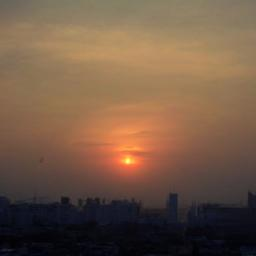
\includegraphics[width=0.32\linewidth]{figs/samples/cfg_prompt_49_image_5.jpg}\;%
        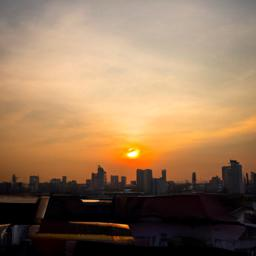
\includegraphics[width=0.32\linewidth]{figs/samples/cfg_prompt_49_image_7.jpg}\\
        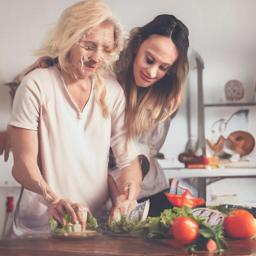
\includegraphics[width=0.32\linewidth]{figs/samples/cfg_prompt_1_image_0.jpg}\;%
        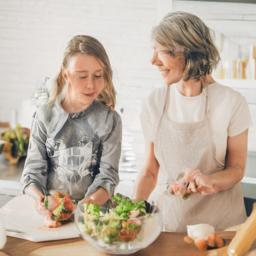
\includegraphics[width=0.32\linewidth]{figs/samples/cfg_prompt_1_image_1.jpg}\;%
        
\includegraphics[width=0.32\linewidth]{figs/samples/cfg_prompt_1_image_8.jpg}
    \end{subfigure}
    \begin{subfigure}[t]{0.495\linewidth}
        \centering
        \caption*{\textbf{Adjoint Matching (Ours)}}
        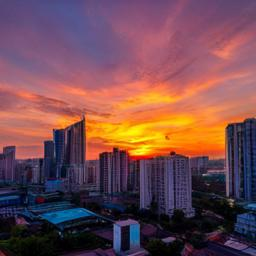
\includegraphics[width=0.32\linewidth]{figs/samples/adjmat_prompt_49_image_1.jpg}\;%
        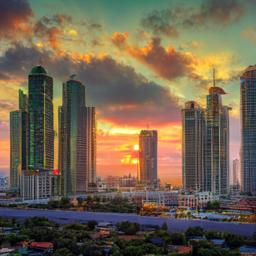
\includegraphics[width=0.32\linewidth]{figs/samples/adjmat_prompt_49_image_5.jpg}\;%
        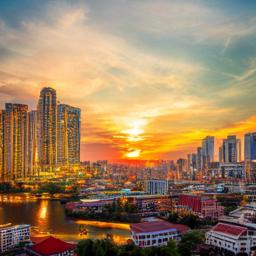
\includegraphics[width=0.32\linewidth]{figs/samples/adjmat_prompt_49_image_7.jpg}\\
        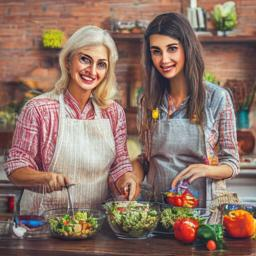
\includegraphics[width=0.32\linewidth]{figs/samples/adjmat_prompt_1_image_0.jpg}\;%
        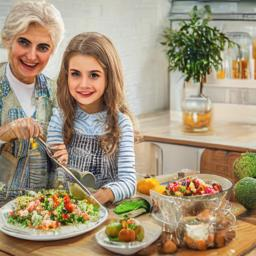
\includegraphics[width=0.32\linewidth]{figs/samples/adjmat_prompt_1_image_1.jpg}\;%
        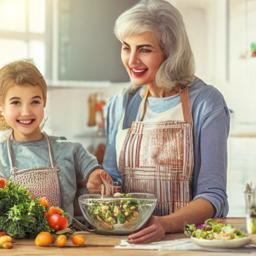
\includegraphics[width=0.32\linewidth]{figs/samples/adjmat_prompt_1_image_8.jpg}
    \end{subfigure}\\
    \begin{subfigure}[t]{0.495\linewidth}
        \centering
        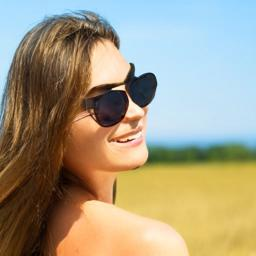
\includegraphics[width=0.32\linewidth]{figs/samples/cfg_prompt_72_image_0.jpg}\;%
        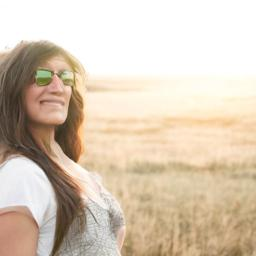
\includegraphics[width=0.32\linewidth]{figs/samples/cfg_prompt_72_image_1.jpg}\;%
        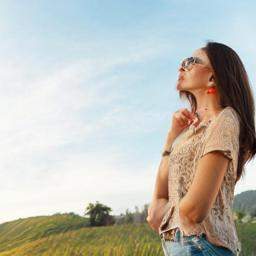
\includegraphics[width=0.32\linewidth]{figs/samples/cfg_prompt_72_image_6.jpg}\\
        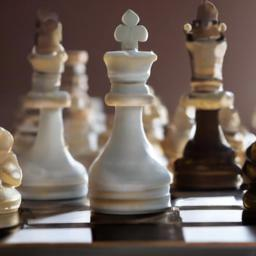
\includegraphics[width=0.32\linewidth]{figs/samples/cfg_prompt_75_image_0.jpg}\;%
        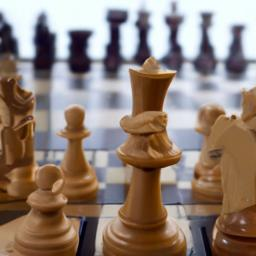
\includegraphics[width=0.32\linewidth]{figs/samples/cfg_prompt_75_image_3.jpg}\;%
        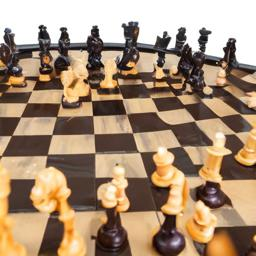
\includegraphics[width=0.32\linewidth]{figs/samples/cfg_prompt_75_image_9.jpg}
    \end{subfigure}
    \begin{subfigure}[t]{0.495\linewidth}
        \centering
        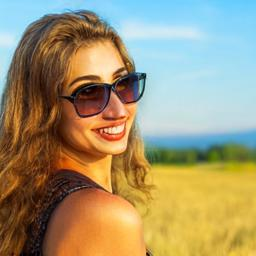
\includegraphics[width=0.32\linewidth]{figs/samples/adjmat_prompt_72_image_0.jpg}\;%
        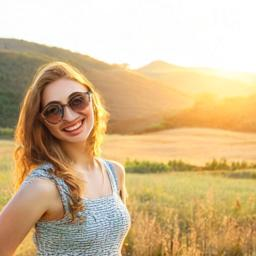
\includegraphics[width=0.32\linewidth]{figs/samples/adjmat_prompt_72_image_1.jpg}\;%
        
\includegraphics[width=0.32\linewidth]{figs/samples/adjmat_prompt_72_image_6.jpg}\\
        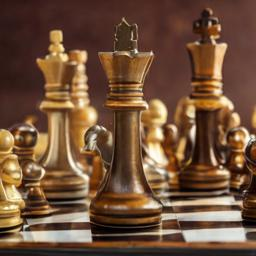
\includegraphics[width=0.32\linewidth]{figs/samples/adjmat_prompt_75_image_0.jpg}\;%
        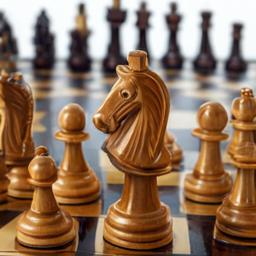
\includegraphics[width=0.32\linewidth]{figs/samples/adjmat_prompt_75_image_3.jpg}\;%
        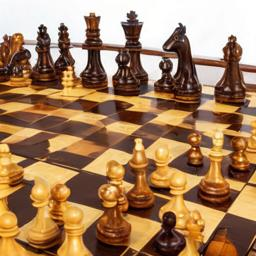
\includegraphics[width=0.32\linewidth]{figs/samples/adjmat_prompt_75_image_9.jpg}
    \end{subfigure}\\
    \caption{We introduce Adjoint Matching, a theoretically-driven yet simple algorithm for reward fine-tuning that works for a large family of dynamical generative models, including for the first time, Flow Matching models. 
    Text prompts: ``\textit{Beautiful colorful sunset midst of building in Bangkok Thailand}'', ``\textit{Beautiful grandma and granddaughter are mixing salad and smiling while cooking in kitchen}'', ``\textit{The beautiful young woman in sunglasses is standing at the background of field and hill. She is smiling and looking over shoulder}'', ``\textit{Chess, intellectual games, figure horse, chess board}''. 
    }
    \vspace{-6em}
    \label{fig:fig1}
\end{figure}

Flow Matching \citep{lipman2023flow,albergo2023building,liu2023flow} and denoising diffusion
\citep{song2019generative,ho2020denoising,song2021scorebased,kingma2021ondensity}
models are being used for many generative modeling applications, including text-to-image \citep{rombach2022high,esser2024scaling}, text-to-video \citep{singer2022make}, and text-to-audio \citep{le2024voicebox,vyas2023audiobox}. 
In most cases, the base generative model does not achieve the desired sample quality.
To improve the generated samples, it is common to resort to techniques such as classifier-free guidance \citep{ho2022classifier,zheng2023guided} to get better text-to-sample alignment, or to fine-tune using human preference reward models to improve sample quality and realism \citep{wallace2023diffusion,clark2024directly}.

In the adjacent field of large language models, the behavior of the model is aligned to human preferences through fine-tuning with reinforcement learning from human feedback (RLHF).  
Either explicitly or implicitly, RLHF methods \citep{ziegler2020finetuning,stiennon2020learning,ouyang2022training,bai2022training} assume a reward model $r(x)$ that captures human preferences, with the goal of modifying the base generative model such that it generates the following \emph{tilted distribution}: 
\begin{talign} \label{eq:p_star_info}
p^*(x) \propto p^{\mathrm{base}}(x) \exp(r(x)),
\end{talign}
where $p_{\mathrm{base}}$ is the base generative model's sample distribution. 

Inspired by this,
fine-tuning methods have been developed to improve denoising diffusion models based on human preference data; either using a reward-based approach \citep{fan2023optimizing,black2024training,fan2023dpok,xu2023imagereward,clark2024directly,uehara2024understanding,uehara2024finetuning},
or direct preference optimization \citep{wallace2023diffusion}. 
However, unlike the fine-tuning methods designed for large language models,
most of the existing methods to a large degree ignore $p^\text{base}$ and focus solely on the reward model.
Reward models can range from standard evaluation metrics such as ClipScore \citep{hessel2021clipscore,kirstain2023pickapic} to specialized models that have been trained on human preferences \citep{schuhmann2022laion,xu2023imagereward,wu2023humanpreferencescorev2}. As these are parameterized by neural networks, they fall pray to adversarial examples which lead to the generation of undesirable artifacts \citep{goodfellow2014explaining,mordvintsev2015inceptionism}. This has led some works to consider adding regularization during fine-tuning \citep{fan2024reinforcement,uehara2024finetuning} to incentivize staying close to the base model distribution; however, there does not yet exist a \emph{simple} approach which actually provably generates from the tilted distribution \eqref{eq:p_star_info}. 

The main contributions of our paper are as follows:
\begin{enumerate}[label=(\roman*)]
    \item We present a stochastic optimal control (SOC) formulation for reward fine-tuning of dynamical generative models. Importantly, we prove that the na\"ive approach considered by prior works lead to a \emph{value function bias} problem that biases the fine-tuned model away from the tilted distribution \eqref{eq:p_star_info}. 
    This problem has also been observed by \citet{uehara2024finetuning} but they propose a more complicated solution which involves training a separate generative model for the optimal noise distribution.
    \item Instead, we propose a very simple solution: the \emph{memoryless noise schedule}. This is a unique noise schedule that completely removes the dependency between noise variables and the generated samples, resulting in provable convergence to the tilted distribution. 
    This allows us to fine-tune dynamical generative models in full generality, including being the first to fine-tune noiseless Flow Matching models.
    \item We also propose a new method for solving SOC problems, called \emph{Adjoint Matching}, which combines the scalability of gradient-based methods and the simplicity of a least-squares regression objective. This is orthogonal to the reward fine-tuning application and can be applied to general SOC problems.
    \item We perform extensive comparisons to baseline approaches, and analyze them from multiple perspectives such as realism, consistency, and diversity. We find that our proposed method provides generalization to unseen human preference reward models, better text-to-sample consistency, and retains good diversity.
\end{enumerate}
In the following, sections are broken down as follows: \Cref{sec:prelim_generative_models} summarizes the algorithms used for sampling from pre-trained Flow Matching and diffusion models, while \Cref{sec:common_perspective} provides a common notation that we will use throughout. \Cref{sec:memoryless_SOC,sec:adjoint_matching} form the core of our contributions. \Cref{sec:memoryless_SOC} details the value function bias problem and our proposed solution via the memoryless noise schedule. \Cref{sec:adjoint_matching} details the new Adjoint Matching algorithm for solving SOC problems. 
%Within each section, we first present preliminaries that summarize the existing methods and their relation to our contributions. 

\section{Preliminaries on dynamical generative models}\label{sec:prelim_generative_models}

We are interested in fine-tuning base generative models $p^{\mathrm{base}}(X_1)$ where samples are generated through the simulation of a stochastic process. That is, these models transform noise variables into a sample through an iterative process. In particular, we discuss the specific constructions and sampling processes of Flow Matching~\citep{lipman2023flow,liu2023flow,liu2022rectified,albergo2023building} and Denoising Diffusion Models~\citep{ho2020denoising,song2021scorebased,song2021denoising}.
The goal of this section is to provide background information on these methods, which we will later unify into a single consistent notation in \Cref{sec:common_perspective}.

Given random variables from an initial distribution $\bar{X}_0 \sim p_0 = \mathcal{N}(0, I)$, and $\bar{X}_1$ which are distributed according to some data distribution, we define the reference flow $\bm{\bar{X}} = (\bar{X}_t)_{t\in[0,1]}$ where
\begin{talign} \label{eq:reference_flow}
\bar{X}_t = \beta_t \bar{X}_0 + \alpha_t \bar{X}_1,
\end{talign}
where $(\alpha_t)_{t \in [0,1]}, (\beta_t)_{t \in [0,1]}$ are functions such that $\alpha_0 = \beta_1 = 0$ and $\alpha_1 = \beta_0 = 1$. 
Diffusion models and Flow Matching construct generative Markov processes $X_t$ with initial distribution $X_0 \sim \mathcal{N}(0, I)$ that result in flows $\bm{X} = (X_t)_{t \in [0,1]}$ with the same time marginals as the reference flow $\bm{\bar{X}}$, \ie, the random variables $X_t$ and $\bar{X}_t$ have identical distribution for all times $t \in [0, 1]$. 
This implies $X_1$ has the same distribution as the data distribution, so simulating the Markov process from random noise $X_0$ is a way to generate artificial samples\footnote{In our derivations, we will simply assume the base model has been trained perfectly during the pre-training phase.}.

\subsection{Flow Matching}

In its simplest form, the generative Markov process of a Flow Matching model is an ordinary differential equation (ODE) of the form:
\begin{talign} \label{eq:FM_ode}
    \mathrm{d}X_t = v
    %^\text{base}
    (X_t,t) \, \mathrm{d}t, \qquad X_0 \sim \mathcal{N}(0,I).
\end{talign}
where $v(X_t, t)$ is a parametric velocity that is optimized to match the derivative of the reference flow, \ie,
%\begin{talign}
$v
% ^\text{base}
(X_t, t) = \argmin_{\hat{v}} \mathbb{E} \big\| \hat{v}(\bar{X}_t,t) - \frac{\mathrm{d}}{\mathrm{d}t}\bar{X}_t \big\|^2$ (see \eg \citet{lipman2023flow} for details on pre-training Flow Matching models).
%\end{talign}
It can then be proven that the solution of the generative process \eqref{eq:FM_ode} has the same time marginals as the reference flow \citep{lipman2023flow,liu2022rectified,albergo2023building}, and a commonly used choice is $\alpha_t = t$ and $\beta_t = 1-t$.
One can also consider a family of stochastic differential equations (SDEs) with an arbitrary state-independent diffusion coefficient%
\footnote{We use the common short-hand ``over-dot'' notation to denote the time derivative, \ie, $\dot{x}_t = \frac{\mathrm{d}}{\mathrm{d}t} x_t$.}%
:
\begin{talign} \label{eq:FM_general_diffusion_coeff}
    \mathrm{d}X_t = \left( v
    % ^\text{base}
    (X_t,t) + \frac{\sigma(t)^2}{2\beta_{t}(\frac{\dot{\alpha}_{t}}{\alpha_{t}} \beta_{t} -\dot{\beta}_{t})} \left( v
    % ^\text{base}
    (X_t,t) - \frac{\dot{\alpha}_{t}}{\alpha_{t}} X_t \right) \right) \, \mathrm{d}t + \sigma(t) \, \mathrm{d}B_t, \qquad X_0 \sim \mathcal{N}(0,I),
\end{talign}
where $(B_t)_{t\geq 0}$ is a Brownian motion.
The generative processes in \eqref{eq:FM_ode} and \eqref{eq:FM_general_diffusion_coeff} have the same time marginals. This can be seen by writing down the Fokker-Planck equations for \eqref{eq:FM_ode} and \eqref{eq:FM_general_diffusion_coeff}, and observing that they are the same up to a cancellation of terms~\citep{maoutsa2020interacting}.
The diffusion coefficient $\sigma(t)$ in \eqref{eq:FM_general_diffusion_coeff} is compensated by the second term in the drift which scales proportionally as $\sigma(t)^2$. 

% To simulate the SDE \eqref{eq:FM_general_diffusion_coeff}, a good approach is to consider a $K$-step discretization: for $k\in \{0,\dots,K\}$,
% \begin{talign} \label{eq:FM_discretization}
%     X_{k+1} = X_k + \frac{1}{K} v
%     % ^\text{base}
%     (X_k,\frac{k}{K}) + \frac{K \sigma_k^2}{2\beta_{k}\left(\frac{\alpha_{k+1} - \alpha_k}{\alpha_{k}} \beta_{k} - \beta_{k+1} + \beta_{k}\right)} \left( v
%     % ^\text{base}
%     (X_k,\frac{k}{K}) - \frac{\alpha_{k+1} - \alpha_k}{K\alpha_{k}} X_k \right) +
%     \frac{1}{\sqrt{K}} \sigma_{k} \varepsilon_{k},
%     \qquad \substack{\varepsilon_k \sim \mathcal{N}(0,I), \\ X_0 \sim \mathcal{N}(0,I),}
% \end{talign}
% where we've identified the continuous-time process $(X_t)_{t\in[0,1]}$ with a discrete-time process $(X_k)_{k\in\{0,\dots,K\}}$, where $\alpha_k = \alpha(\nicefrac{k}{K})$, $\beta_k = \beta(\nicefrac{k}{K})$, and $\sigma_k = \sigma(\nicefrac{k}{K})$, applied a first-order approximation.

\subsection{Denoising Diffusion Models}

We next discuss diffusion models, in particular the sampling scheme proposed by Denoising Diffusion Implicit Model (DDIM; \cite{song2021denoising}) which we will later relate to Denoising Diffusion Probabilistic Models (DDPM; \cite{ho2020denoising}) as a particular case of the former. 
For sampling from a diffusion model, the DDIM update rule%
\footnote{We slightly depart from the notation in \citet{song2021denoising} by flipping the direction of time and using $\bar{\alpha}_k$ which corresponds to the $\alpha_k$ in \citet{song2021denoising} while it corresponds to the $\bar{\alpha}_k$ in \citet{ho2020denoising}.}~(\citet{song2021denoising}, Eq. 12)%
, typically stated in discrete time with $k\in \{0,\dots,K\}$, is:
\begin{talign} \label{eq:DDIM_original_main}
    X_{k+1} = \sqrt{\bar{\alpha}_{k+1}}
    \big( \frac{X_{k} - \sqrt{1-\bar{\alpha}_k} \epsilon(X_k,k)}{\sqrt{\bar{\alpha}_k}} \big)
    + \sqrt{1-\bar{\alpha}_{k+1} - \sigma_{k}^2} \epsilon(X_k,k) +
    % \frac{1}{\sqrt{K}} 
    \sigma_{k} \varepsilon_{k},
    \qquad \varepsilon_k \sim \mathcal{N}(0,I), \ X_0 \sim \mathcal{N}(0,I),
\end{talign}
where $\bar{\alpha}_k$ is an increasing sequence such that $\bar{\alpha}_0 = 0$, $\bar{\alpha}_K = 1$, and the sequence $\sigma_k$ is arbitrary. That is, one samples an initial Gaussian random variable $x_0$, and applies the stochastic update \eqref{eq:DDIM_original_main} iteratively $K$ times in order to obtain an artificial sample $X_K$. Updates can be interpreted as progressively denoising the iterate: $x_0$ is completely noisy and $x_K$ is fully denoised. The noise predictor model $\epsilon(x_k,k)$ is trained to predict the noise of $x_k$ (see \eg \citet{ho2020denoising} for details on pre-training denoising diffusion models). 

\section{Flow Matching and diffusion models from a common perspective}\label{sec:common_perspective}

We formulate Flow Matching and diffusion models in a unified framework, which we will later use throughout the paper.
Firstly, to simplify notation, we will be using continuous-time formulations. This will also directly enable fine-tuning methods inspired by the continuous-time paradigm, which we find tends to perform better than discrete-time counterparts in our empirical validations. Secondly, by consolidating notation, we will be able to discuss fine-tuning of dynamical generative models that follow the same time marginals as the reference flow \eqref{eq:reference_flow}, pre-trained with either the Denoising Diffusion or Flow Matching framework, in full generality.

To convert DDIM to a continuous-time stochastic process, we can show that the DDIM update rule \eqref{eq:DDIM_original_main}, up to a first-order approximation, is equivalent to the Euler-Maruyama discretization of the following SDE:
\begin{talign} \label{eq:euler_maruyama_DDIM}
    \mathrm{d}X_t &= \big( \frac{\dot{\bar{\alpha}}_{t}}{2\bar{\alpha}_{t}} X_t - \big( \frac{\dot{\bar{\alpha}}_{t}}{2\bar{\alpha}_{t}} + \frac{\sigma(t)^2}{2} \big) \frac{\epsilon^\text{base}(X_{t},t)}{\sqrt{1-\bar{\alpha}_{t}}} \big) \mathrm{d}t + \sigma(t) \mathrm{d}B_t, \qquad X_{0} \sim \mathcal{N}(0,I).
\end{talign}
See \Cref{subsec:continuous_DDIM} for the full derivation.
To go from \eqref{eq:DDIM_original_main} to \eqref{eq:euler_maruyama_DDIM}, we assumed a uniform discretization of time, \ie $t=\tfrac{k}{K}$. 
This results in identifying the discrete-time process $(X_{k})_{k\in \{0,\dots,K\}}$ with a continuous-time process $(X_{t})_{t\in[0, 1]}$, where $\bar{\alpha}_k := \bar{\alpha}_{t}$, $\sigma_k := \frac{1}{\sqrt{K}} \sigma(t)$, and $\epsilon(X_k, k)$ with $\epsilon^\text{base}(X_k, t)$. 
In relation to the reference flow \eqref{eq:reference_flow}, the generative process in \eqref{eq:euler_maruyama_DDIM} has the same time marginals when $\alpha_t = \sqrt{\bar{\alpha}_t}$ and $\beta_t = \sqrt{1 - \bar{\alpha}_t}$~\citep{ho2020denoising}.

Furthermore, when viewed up to first order approximations, the DDPM sampling scheme~(\citet{ho2020denoising}; Algorithm 2) can be seen as special instance of the DDIM sampling scheme when $\sigma(t) = \sqrt{\nicefrac{\dot{\bar{\alpha}}_t}{\bar{\alpha}_t}}$. This results in the following generative process:
\begin{talign}\label{eq:euler_maruyama_DDPM}
    \mathrm{d}X_t &= \big( \frac{\dot{\bar{\alpha}}_{t}}{2\bar{\alpha}_{t}} X_t - \frac{\dot{\bar{\alpha}}_{t}}{\bar{\alpha}_{t}} \frac{\epsilon^\text{base}(X_{t},t)}{\sqrt{1-\bar{\alpha}_{t}}} \big) \mathrm{d}t + \sqrt{\frac{\dot{\bar{\alpha}}_{t}}{\bar{\alpha}_{t}}} \mathrm{d}B_t, \qquad X_{0} \sim \mathcal{N}(0,I),
\end{talign}
% We defer the derivation of the continuous-time limit of DDPM to \Cref{eq:euler_maruyama_DDIM}.

We can further consolidate notation by converting all quantities to the score function $\mathfrak{s}(x,t)$---defined as the gradient of the log density of the random variable $X_t$---which is possible when $X_0$ is Normal-distributed and under the affine reference flow \eqref{eq:reference_flow}. In particular, 
the velocity $v^\text{base}$ from Flow Matching can be expressed in terms of the score function (see \Cref{subsec:v_score}):
\begin{talign}
    v^\text{base}(x,t) = \frac{\dot{\alpha}_t}{\alpha_t} x + \beta_t(\frac{\dot{\alpha}_t}{\alpha_t} \beta_t - \dot{\beta}_t) \mathfrak{s}(x,t).
\end{talign}
And the noise predictor $\epsilon^\text{base}$ also admits an expression in terms of the score function (see \Cref{subsec:hat_epsilon_score}):
\begin{talign}
    \mathfrak{s}(x,t) = - \frac{\epsilon^\text{base}(x,t)}{\sqrt{1-\bar{\alpha}_t}}.
\end{talign}
Plugging these two equations into \eqref{eq:FM_general_diffusion_coeff} and \eqref{eq:euler_maruyama_DDIM}, respectively, and rewriting them in terms of only the $\alpha_t$ and $\beta_t$ in \eqref{eq:reference_flow}, we can unify both the Flow Matching and continuous-time DDIM generative processes as:
\begin{talign} \label{eq:gen_process_1}
    \mathrm{d}X_t &= b(X_t,t) \, \mathrm{d}t + \sigma(t) \, \mathrm{d}B_t, \qquad X_0 \sim \mathcal{N}(0,I), \\
    \text{where} \ b(x,t) &= \kappa_t x + \big(\frac{\sigma(t)^2}{2} + \eta_t\big) \mathfrak{s}(x,t), \quad \kappa_t = \frac{\dot{\alpha}_t}{\alpha_t}, \quad 
    \eta_t = \beta_t (\frac{\dot{\alpha}_t}{\alpha_t} \beta_t - \dot{\beta}_t)
    \label{eq:gen_process_2}
\end{talign}
where $(\alpha_t, \beta_t)$ are coefficients of the reference flow \eqref{eq:reference_flow}. We have hence expressed the generative process of a base model, whether it is a Flow Matching or a diffusion model, as an SDE of the form \eqref{eq:gen_process_1}-\eqref{eq:gen_process_2}, unified by the choice of reference flow. This expression has been written before for DDIM, e.g. \cite{bartosh2024neural,bartosh2024neural2}.
%Cref{tab:coefficients} summarizes the coefficients for each pre-training framework.

\section{Fine-tuning as ``memoryless'' stochastic optimal control}
\label{sec:memoryless_SOC}

We now discuss the crux of the problem: how to produce a fine-tuned generative model that produces samples $X_1$ which follow the tilted distribution involving a reward model \eqref{eq:p_star_info}. 
An obvious direction is to construct a \emph{fine-tuning objective} involving both the base generative model and the reward model, where the optimal solution results in a fine-tuned generative model for the tilted distribution. 
However, as we will explain, this turns out to be non-trivial, because a na\"ive formulation will introduce bias into the solution.

In \Cref{sec:SOC_formulation}, we discuss the problem formulation of stochastic optimal control, a general framework for optimizing SDEs, and its relation to the maximum entropy reinforcement learning framework commonly used for RLHF fine-tuning. 
Next, in \Cref{sec:value_function_bias_problem}, we discuss the \emph{initial value function bias} problem which plagues existing approaches and so far has seen no simple solution.
Finally, in \Cref{sec:memoryless_schedule}, we propose a novel simple solution that circumvents the bias problem, by enforcing a particular diffusion coefficient, the \emph{memoryless noise schedule}, to be used during fine-tuning. This results in an extremely simple fine-tuning objective that provably converges to a model which generates the tilted distribution \eqref{eq:p_star_info} without any statistical bias.

% However, this turns out to not be trivial. As a na\"ive formulation will add bias into the solution, or simply shift the problem into optimizing the base distribution of the generative model.

\subsection{Preliminaries on the stochastic optimal control problem formulation} \label{sec:SOC_formulation}

Stochastic optimal control (SOC; \cite{bellman1957,fleming2012deterministic,sethi2018optimal}) considers general optimization problems over stochastic differential equations, but we only need to consider a common instantiation, the quadratic cost control-affine problem formulation:
\graybox{
\begin{talign} \label{eq:control_problem_def}
    &\min\limits_{u \in \mathcal{U}} \mathbb{E} \big[ \int_0^1 
    \big(\frac{1}{2} \|u(X^u_t,t)\|^2 + f(X^u_t,t) \big) \, \mathrm{d}t + 
    g(X^u_1) \big], \\
    \begin{split}
    \text{s.t.}~ \mathrm{d}X^u_t =  \left( b(X^u_t,t) + \sigma(t) u(X^u_t,t) \right) \, \mathrm{d}t + 
    \sigma(t) \mathrm{d}B_t, \qquad X^u_0 \sim p_0
    \end{split} 
    \label{eq:controlled_SDE}
\end{talign}
}
where in \eqref{eq:controlled_SDE}, $X_t^u \in \R^d$ is the state of the stochastic process, $u : \R^d \times [0,1] \to \R^d$ is commonly referred to as the control vector field, $b : \R^d \times [0,1] \to \R^d$ is a base drift, and $\sigma : [0,1] \to \R^{d \times d}$ is the diffusion coefficient. These jointly define the \emph{controlled process} $\fX^u \sim p^u$ that we are interested in optimizing; often both $b$ and $\sigma$ are fixed and we only optimize over the control $u$. 

As part of the objective functional \eqref{eq:control_problem_def}, we have an affine control cost $\frac{1}{2} \|u(X^u_t,t)\|^2$, a running state cost $f : \R^d \times [0,1] \to \R$ and a terminal state cost $g : \R^d \to \R$. 
%For the application of RLHF to dynamical generative models, we only need to consider the case of $f=0$; however, we will keep $f$ in the discussion for full generality as our proposed Adjoint Matching algorithm (\Cref{sec:adjoint_matching}) solves any control-affine SOC problem formulation.

The stochastic optimal control (SOC) objective \eqref{eq:control_problem_def} can be decomposed recursively from the final time value. It is common to define the \emph{cost functional} which is the expected future cost starting from state $x$ at time $t$:
\begin{talign} \label{eq:cost_functional}
J(u;x,t) := \mathbb{E}_{\fX \sim p^u} \left[ \int_t^1 
\left(\frac{1}{2} \|u(X_s,s)\|^2  +  f(X_s,s) \right) \, \mathrm{d}s  +  
g(X_1) \;\big|\; X_t = x \right].
\end{talign}
From here, the \emph{value function} is the optimal value of the cost functional%
\footnote{Note that there is a slight difference in terminology between SOC and reinforcement learning, where our cost functional is referred to as the state value function and our value function is the optimal state value function in RL.}
:
\begin{talign}\label{eq:value_fn_defn}
V(x,t) := \min_{u\in \mathcal{U}} J(u;x,t) = J(u^*;x,t),
\end{talign}
where $u^*$ is the \emph{optimal control}, \ie, minimizer of \eqref{eq:control_problem_def}. Furthermore, a classical result is that the value function can be expressed in terms of the \emph{uncontrolled} base process $p^\text{base}$ (\cite{kappen2005path}, see \citealt[Eq.~8,~App.~B]{domingoenrich2023stochastic} for a self-contained proof):
\begin{talign}\label{eq:value_fn_from_uncontrolled}
    V(x, t) = - \log \E_{\fX \sim p^\text{base}} \left[ \exp( - \int_t^1 f(X_s, s) \mathrm{d}s - g(X_1) ) \;\big|\; X_t = x  \right]. 
\end{talign}
A useful expression for the optimal control (which we will make use of in deriving the Adjoint Matching objective in \Cref{sec:adjoint_matching}) is that it is related to the gradient of the value function:
\begin{talign} \label{eq:optimal_control}
u^*(x,t) = - \sigma(t)^{\top} \nabla_x V(x,t) = - \sigma(t)^{\top} \nabla_x J(u^*, x,t).
\end{talign}
%
\paragraph{Relation to MaxEnt RL.} Stochastic optimal control with the control-affine formulation \eqref{eq:control_problem_def} is the continuous-time equivalence of maximum entropy reinforcement learning (MaxEnt RL; \citet{todorov2006linearly,ziebart2008maximum}) with a KL regularization instead of only an entropy regularization. In particular, by the Girsanov theorem (\Cref{cor:girsanov_sdes}), 
% \ricky{cite}, 
the affine control cost is equivalent to a Kullback–Leibler (KL) divergence between the base process $p^\text{base}$, when $u=0$, and the controlled process $p^u$, when conditioned on the same initial state $X_0$ (see \Cref{subsec:proof_eq_cond_kl}):
\begin{talign}\label{eq:cond_kl}
    \infdiv*{p^u(\fX | X_0)}{p^{base}(\fX | X_0)} = \mathbb{E}_{\fX^u \sim p^u} \left[ \int_{0}^1 \frac{1}{2} \|u(X^u_t,t)\|^2 \mathrm{d}t \right],
\end{talign}
resulting in the KL-regularized RL interpretation of \eqref{eq:control_problem_def}:
\begin{talign}\label{eq:kl_regularized_interpretation}
    &\max\limits_{u \in \mathcal{U}}\;
    \E_{X_0 \sim p_0} \left[
    \mathbb{E}_{\fX \sim p^u(\cdot | X_0)} \big[ \int_0^1  -f(X_t^u , t) \mathrm{d} t - g(X_1^u) \big] - \infdiv{p^u(\fX | X_0)}{p^{base}(\fX | X_0)}
    \right],
\end{talign}
where the negative state costs correspond to intermediate and terminal rewards in the RL interpretation. The KL divergence incentivizes the optimal solution to stay close to the distribution of the base process. 
%This KL regularization is a common objective for RLHF of large language models \citep{ouyang2022training} but has seen seldom use in fine-tuning diffusion models, particularly due to a problem that we will discuss next.

\subsection{The initial value function bias problem} \label{sec:value_function_bias_problem}

We next discuss why na\"ively adding a KL regularization does not lead to the tilted distribution \eqref{eq:p_star_info}.
From \eqref{eq:kl_regularized_interpretation}, we can also show that the optimal distribution conditioned on $X_0$ is%
\footnote{Note \eqref{eq:cond_optimal_distribution_SOC} is informal because densities over continuous-time processes are ill-defined; the formal statement is $\frac{\mathrm{d}\mathbb{P}^{*}}{\mathrm{d}\mathbb{P}^{\mathrm{base}}}(\fX | X_0) = \exp ( - \int_0^1 f(X_t,t) \, \mathrm{d}t - g(X_1))$, where $\frac{\mathrm{d}\mathbb{P}^{*}}{\mathrm{d}\mathbb{P}^{\mathrm{base}}}$ denotes the Radon-Nikodym derivative. We treat this formally in the proofs.}
\begin{talign}\label{eq:cond_optimal_distribution_SOC}
    p^{*}(\fX | X_0) \propto 
    p^{\mathrm{base}}(\fX | X_0) \exp \big( - \int_0^1 f(X_t,t) \, \mathrm{d}t - g(X_1) \big).
\end{talign}
This is analogous to the exponentiated reward distribution in MaxEnt RL \citep{rawlik2013stochastic}, but since we generalize the entropy regularization to a KL regularization, $p^\text{base}$ acts as a prior distribution.

% Importantly, 
In order to relate this to the tilted distribution \eqref{eq:p_star_info} that we want to achieve for fine-tuning, 
% we need to marginalize all time values and check the distribution of $p^*(X_1)$. In order to do this, 
first notice that the normalization constant of the right-hand side (RHS) of \eqref{eq:cond_optimal_distribution_SOC} is exactly the value function at $t=0$:
\begin{talign}\label{eq:normalization_constant}
    \E_{\fX \sim p^\text{base}(\fX | X_0)} \left[ \exp \big( - \int_0^1 f(X_t,t) \, \mathrm{d}t - g(X_1) \big) \right] = \exp \left( - V(X_0, 0) \right),
\end{talign}
where the equality is due to \eqref{eq:value_fn_from_uncontrolled}.  
% Therefore, we see that this normalization constant depends on $X_0$. 
Dividing the RHS of \eqref{eq:cond_optimal_distribution_SOC} by \eqref{eq:normalization_constant} and multiplying by $p_0(X_0)$, we obtain the normalized distribution over the full path $\fX$,
\begin{talign} \label{eq:optimal_distribution_SOC} 
    p^{*}(\bm{X}) = 
    p^{\mathrm{base}}(\bm{X}) \exp \big( - \int_0^1 f(X_t,t) \, \mathrm{d}t - g(X_1) + V(X_0,0) \big).
\end{talign}
Setting $f=0$ and $g = -r$, we arrive at an expression for the optimal distribution
\begin{talign} \label{eq:optimal_distribution_SOC_RLHF} 
    p^{*}(X_0, X_1) = 
    p^{\mathrm{base}}(X_0, X_1) \exp \big( r(X_1) + V(X_0,0) \big).
\end{talign}
This unfortunately does not lead to the tilted distribution \eqref{eq:p_star_info} because we have a bias in the optimal distribution that is due to the value function of the initial distribution $V(X_0, 0)$. That is to say, na\"ively adding a KL regularization \eqref{eq:cond_kl} to the fine-tuning objective in the sense of \eqref{eq:kl_regularized_interpretation} leads to a biased distribution \eqref{eq:optimal_distribution_SOC} after fine-tuning and is \textit{not} equivalent to the tilted distribution \eqref{eq:p_star_info}. For instance, when the sampling procedure is noiseless, \ie, $\sigma(t) = 0$, fine-tuning na\"ively will not have any effect because $X_0$ completely determines $X_1$.

This is unlike the situation for large language models \citep{ouyang2022training,rafailov2023direct}, where there is no dynamical process that samples $X_1$ iteratively and hence no dependence on the initial noise variable $X_0$. 
Although this KL regularization is a common objective for RLHF of large language models, it has seen seldom use in fine-tuning diffusion models, likely due to this issue of the initial value function bias.

In the context of diffusion models, KL regularization \eqref{eq:kl_regularized_interpretation} has been explored in prior works \citep{fan2024reinforcement}, but its behavior was not well-understood and they did not relate the fine-tuned model to the tilted distribution \eqref{eq:p_star_info}. Another direction that has been proposed is to learn the initial distribution $p_0$ to cancel out the bias \citep{uehara2024finetuning,tang2024finetuning} but this simply shifts the work into tilting the initial distribution and requires an auxiliary model for parameterizing the optimal initial distribution. 
In contrast, we show in the next section that it is possible to remove the value function bias by simply choosing a very particular noise schedule during the fine-tuning procedure. 
% In Figure \Cref{fig:memorylessness_illustration}, we show that this value function bias can introduce arbitrary bias into the fine-tuned distribution depending on different choices of noise schedules.

\subsection{The memoryless noise schedule for fine-tuning dynamical generative models} \label{sec:memoryless_schedule}

\begin{table}
\centering
\begin{tabular}{lcccc}
    \toprule
     & $\kappa_t$ & $\eta_t$ & Diffusion coefficient $\sigma(t)$ & Memoryless $X_t$ \\
    \midrule
    \addlinespace
    Flow Matching \eqref{eq:FM_ode} & $\frac{\dot{\alpha}_t}{\alpha_t}$ & $\beta_t \big(\frac{\dot{\alpha}_t}{\alpha_t} \beta_t - \dot{\beta}_t\big)$ & General (commonly $0$) & No \\
    \addlinespace
    Memoryless Flow Matching \eqref{eq:FM_general_diffusion_coeff} & $\frac{\dot{\alpha}_t}{\alpha_t}$ & $\beta_t \big(\frac{\dot{\alpha}_t}{\alpha_t} \beta_t - \dot{\beta}_t\big)$ & $\sqrt{2\eta_t}$ & Yes \\
    \addlinespace
    DDIM \eqref{eq:euler_maruyama_DDIM} & 
    $\frac{\dot{\bar{\alpha}}_{t}}{2\bar{\alpha}_{t}}$
    & 
    $\frac{\dot{\bar{\alpha}}_{t}}{2\bar{\alpha}_{t}}$
    & General (commonly $0$) & No \\
    \addlinespace
    DDPM \eqref{eq:euler_maruyama_DDPM} & 
    $\frac{\dot{\bar{\alpha}}_{t}}{2\bar{\alpha}_{t}}$
    & 
    $\frac{\dot{\bar{\alpha}}_{t}}{2\bar{\alpha}_{t}}$
    & $\sqrt{2\eta_t}$ & Yes \\
    \bottomrule
\end{tabular}
\caption{Diffusion coefficient $\sigma(t)$ and the factors $\kappa_t$, $\eta_t$ for the Flow Matching, Memoryless Flow Matching, DDIM, and DDPM generative processes. When the diffusion coefficient is $\sigma(t) = \sqrt{2\eta_t}$, the generative process is memoryless, \ie, samples $X_1$ will be independent of the initial noise $X_0$.}
\label{tab:coefficients}
\end{table} 

In this section, we propose a very simple method of turning \eqref{eq:optimal_distribution_SOC_RLHF} into the tilted distribution \eqref{eq:p_star_info} through the use of a particular \emph{memoryless} noise schedule.
Throughout, we provide an intuitive explanation of why this noise schedule is sufficient for fine-tuning while discussing the full theoretical result where we show that the memoryless noise schedule is actually not only sufficient but also necessary.

Intuitively, the main reason we cannot arrive at the tilted distribution from \eqref{eq:optimal_distribution_SOC_RLHF} is due to the $p^{\text{base}}(X_0, X_1)$ distribution not factoring into $X_0$ and $X_1$. Hence, we define a memoryless generative process as follows:
%
\begin{definition}[Memoryless generative process]
A generative process of the form \eqref{eq:gen_process_1}-\eqref{eq:gen_process_2} is memoryless if $X_0$ and $X_1$ are independent, \ie, $p^\text{base}(X_0, X_1) = p^\text{base}(X_0) p^\text{base}(X_1)$.
\end{definition}
When the base generative process is memoryless, this implies:
\begin{talign}
    p^{*}(X_1) 
    = \int p^{\text{base}}(X_0) p^{\text{base}}(X_1) \exp( r(X_1) + V(X_0, 0)) \mathrm{d} X_0
    \propto p^\text{base}(X_1) \exp(r(X_1)).
\end{talign}
That is, solving the SOC problem \eqref{eq:control_problem_def}-\eqref{eq:controlled_SDE} with a memoryless base model will result in a fine-tuned model that generates samples $p^*(X_1)$ according to the tilted distribution \eqref{eq:p_star_info}. 
This memoryless property is not satisfied generally by the family of generative processes captured by \eqref{eq:control_problem_def}-\eqref{eq:controlled_SDE}.
For instance, the Flow Matching and DDIM generative processes with zero diffusion coefficient (\ie, $\sigma(t) = 0$) are definitely not memoryless due to $X_0$ and $X_1$ being theoretically invertible.
Below, we provide the sufficient and neccessary condition for the noise schedule in order to have a memoryless generative process.
%\textcolor{red}{Needs to be adapted to new prop. statement.}
%
\begin{proposition}[Memoryless noise schedules] \label{prop:memorylessness_noise_schedule}
    Within the family of generative processes \eqref{eq:gen_process_1}-\eqref{eq:gen_process_2}, a generative process is memoryless if and only if the noise schedule is chosen as: 
    \begin{talign} \label{eq:chi_condition}
        \sigma(t)^2 = 2 \eta_t + \chi(t), \text{ where } \chi : [0,1] \to \R \text{ is s.t. } \forall t \in (0,1], \quad \lim_{t' \to 0^{+}} \alpha_{t'} \exp \big( - \int_{t'}^t \frac{\chi(s)}{2 \beta_{s}^2} \, \mathrm{d}s \big) = 0.
    \end{talign}
    where $\eta_t$ is the coefficient defined in \eqref{eq:gen_process_2} (see also \autoref{tab:coefficients}).
    In particular, we refer to $\sigma(t) = \sqrt{2\eta_t}$ as the memoryless noise schedule.
\end{proposition}
%
Due to the endpoint constraints of $(\alpha_t, \beta_t)$ for the reference flow \eqref{eq:reference_flow}, the memoryless noise schedule $\sigma(t)$ is infinite at $t=0$ and approaches zero at $t=1$. This provides a way for the generative process to mix when close to noise $X_0$ while stay steadying when close to the sample $X_1$. Hence, the sample will have no information about $X_0$ due to the enormous amount of mixing with a large diffusion coefficient.
% We note that \Cref{prop:memorylessness_noise_schedule} is stronger than this simple explanation portrays: the memoryless noise schedule is the \textit{only} noise schedule that allows $X_0$ and $X_1$ to be independent. 
% Intuitively, when the diffusion coefficient is too large, the drift $b(X_t, t)$ must compensate and this can actually result in stronger dependency between states at different time values. 
Furthermore, while we have intuitively justified the memoryless noise schedule through its independence property, our theoretical result is actually even stronger: all generative models of the form \eqref{eq:gen_process_1}-\eqref{eq:gen_process_2} \textit{must} be fine-tuned using the memoryless noise schedule.
We formalize this in the following theorem, which we prove in \Cref{subsec:proof_prop_diff_finetuning}:
\begin{theorem}[Fine-tuning recipe for general noise schedule sampling] \label{thm:general_fine-tuning}
Within the family of generative processes \eqref{eq:gen_process_1}-\eqref{eq:gen_process_2}, in order to allow the use of arbitrary noise schedules and still generate samples according to the tilted distribution \eqref{eq:p_star_info}, the fine-tuning problem \eqref{eq:control_problem_def}-\eqref{eq:controlled_SDE} with $f=0$ and $g=-r$ must be done with the memoryless noise schedule $\sigma(t) = \sqrt{2\eta_t}$.
\end{theorem}
\Cref{thm:general_fine-tuning} states that we \textit{need} to use the memoryless noise schedule for fine-tuning with the SOC objective---or equivalently, the KL regularized reward objective \eqref{eq:kl_regularized_interpretation}.
This is the only noise schedule that retains the relationship between the velocity and score function, allowing the conversion to arbitrary noise schedules (\eg, $\sigma(t) = 0$) after fine-tuning.
It is worth noting that when using the memoryless noise schedule for DDIM, this recovers what we derived as the continuous-time limit of the DDPM generative process \eqref{eq:euler_maruyama_DDPM}. However, the DDPM sampler \citep{ho2020denoising} is not commonly used while the DDIM sampler \citep{song2021denoising} and Flow Matching models typically generate samples using $\sigma(t) = 0$, so an explicit conversion to the memoryless noise schedule is necessary for fine-tuning. 
To the best of our knowledge, we are not aware of any existing works that have proposed a time-varying diffusion coefficient with theoretical guarantees.
\Cref{tab:coefficients} summarizes the memoryless schedule for diffusion and Flow Matching models, which we refer to as Memoryless Flow Matching. In \Cref{fig:memorylessness_illustration}, we visualize fine-tuning a 1D model, where we see that constant $\sigma(t)$ leads to biased distributions whereas the memoryless noise schedule perfectly converges to the tilted distribution \eqref{eq:p_star_info}. 

\begin{figure}
    \centering
    \begin{subfigure}[t]{\linewidth}
        \centering
        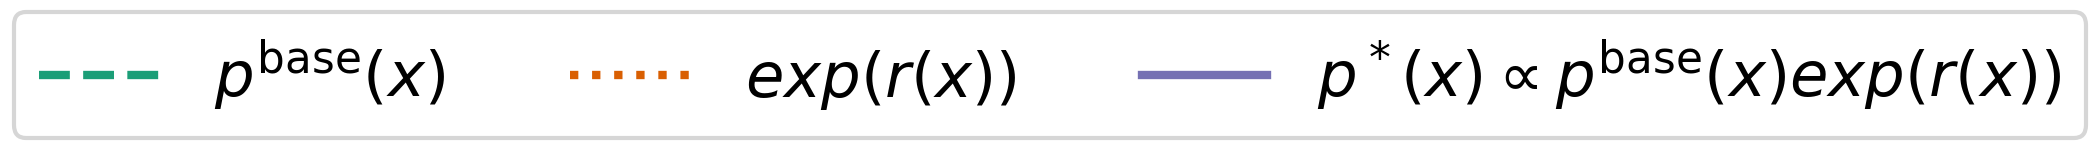
\includegraphics[width=0.7\linewidth]{figs/finetune1d/legend.png}
    \end{subfigure}\\
    \begin{subfigure}[t]{0.25\linewidth}
        \centering
        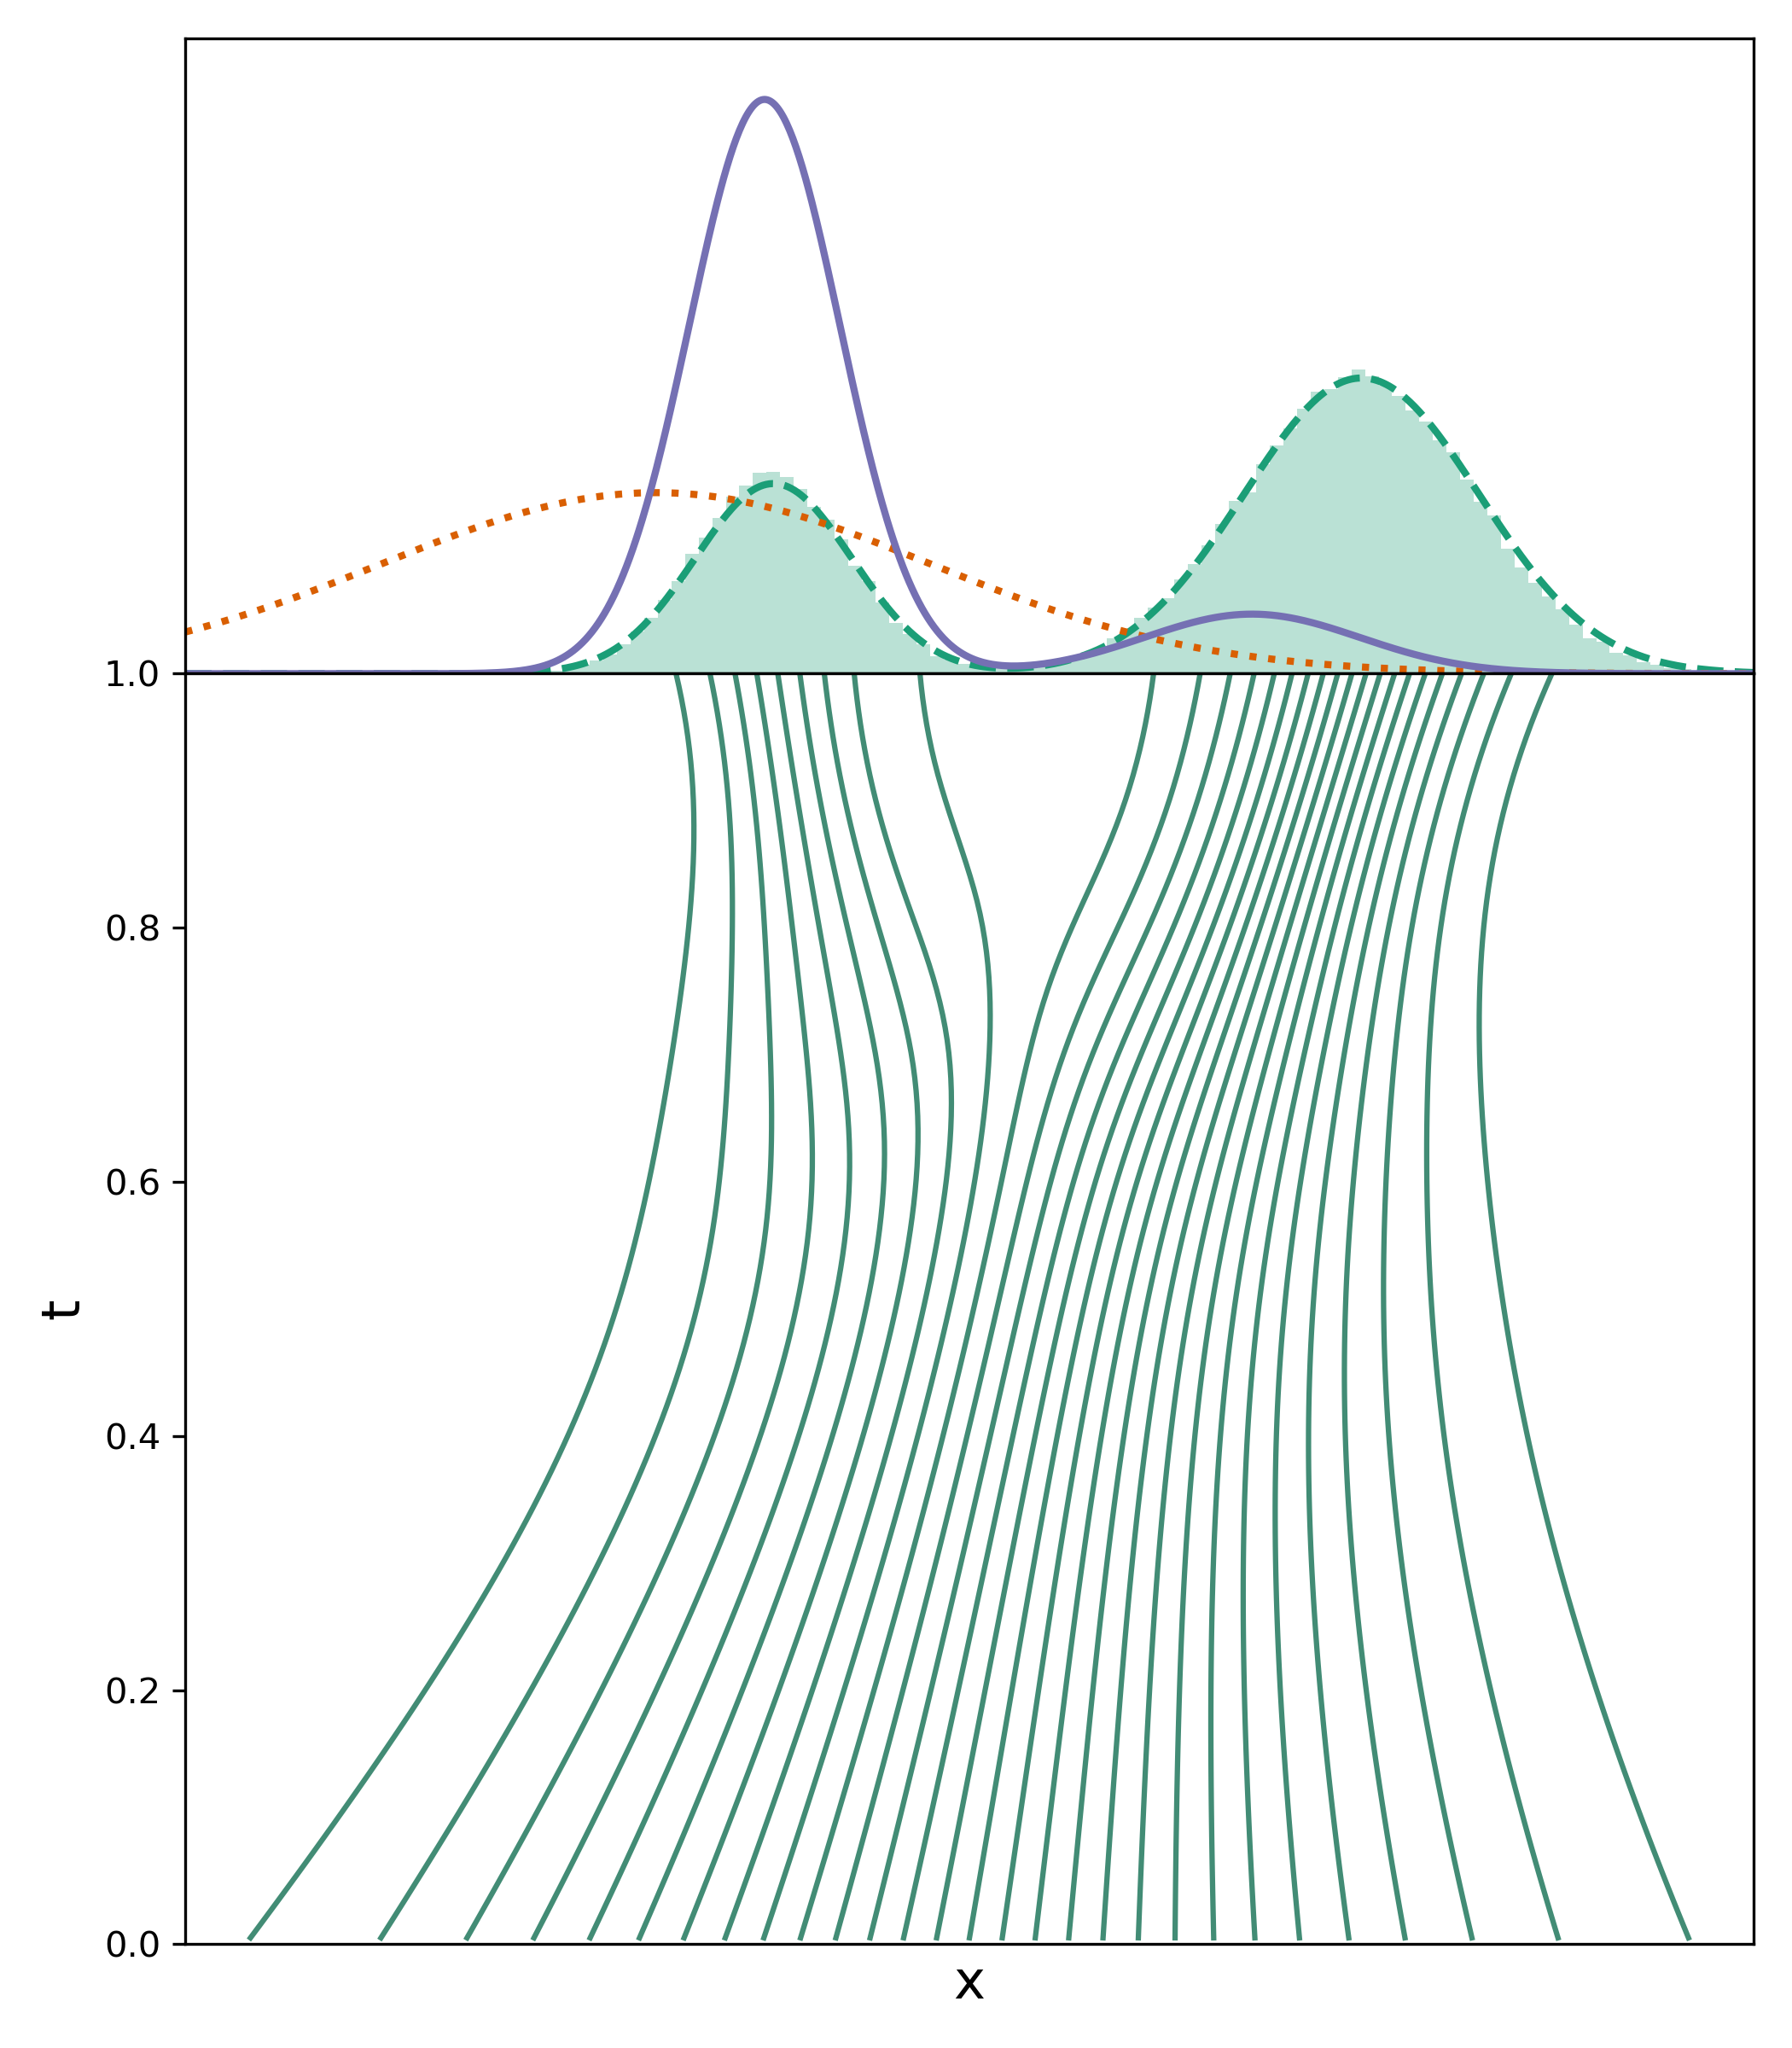
\includegraphics[width=\linewidth]{figs/finetune1d/pretrained_model.png}
        \caption{Pre-trained FM $v^\mathrm{base}$}
    \end{subfigure}%
    \begin{subfigure}[t]{0.25\linewidth}
        \centering
        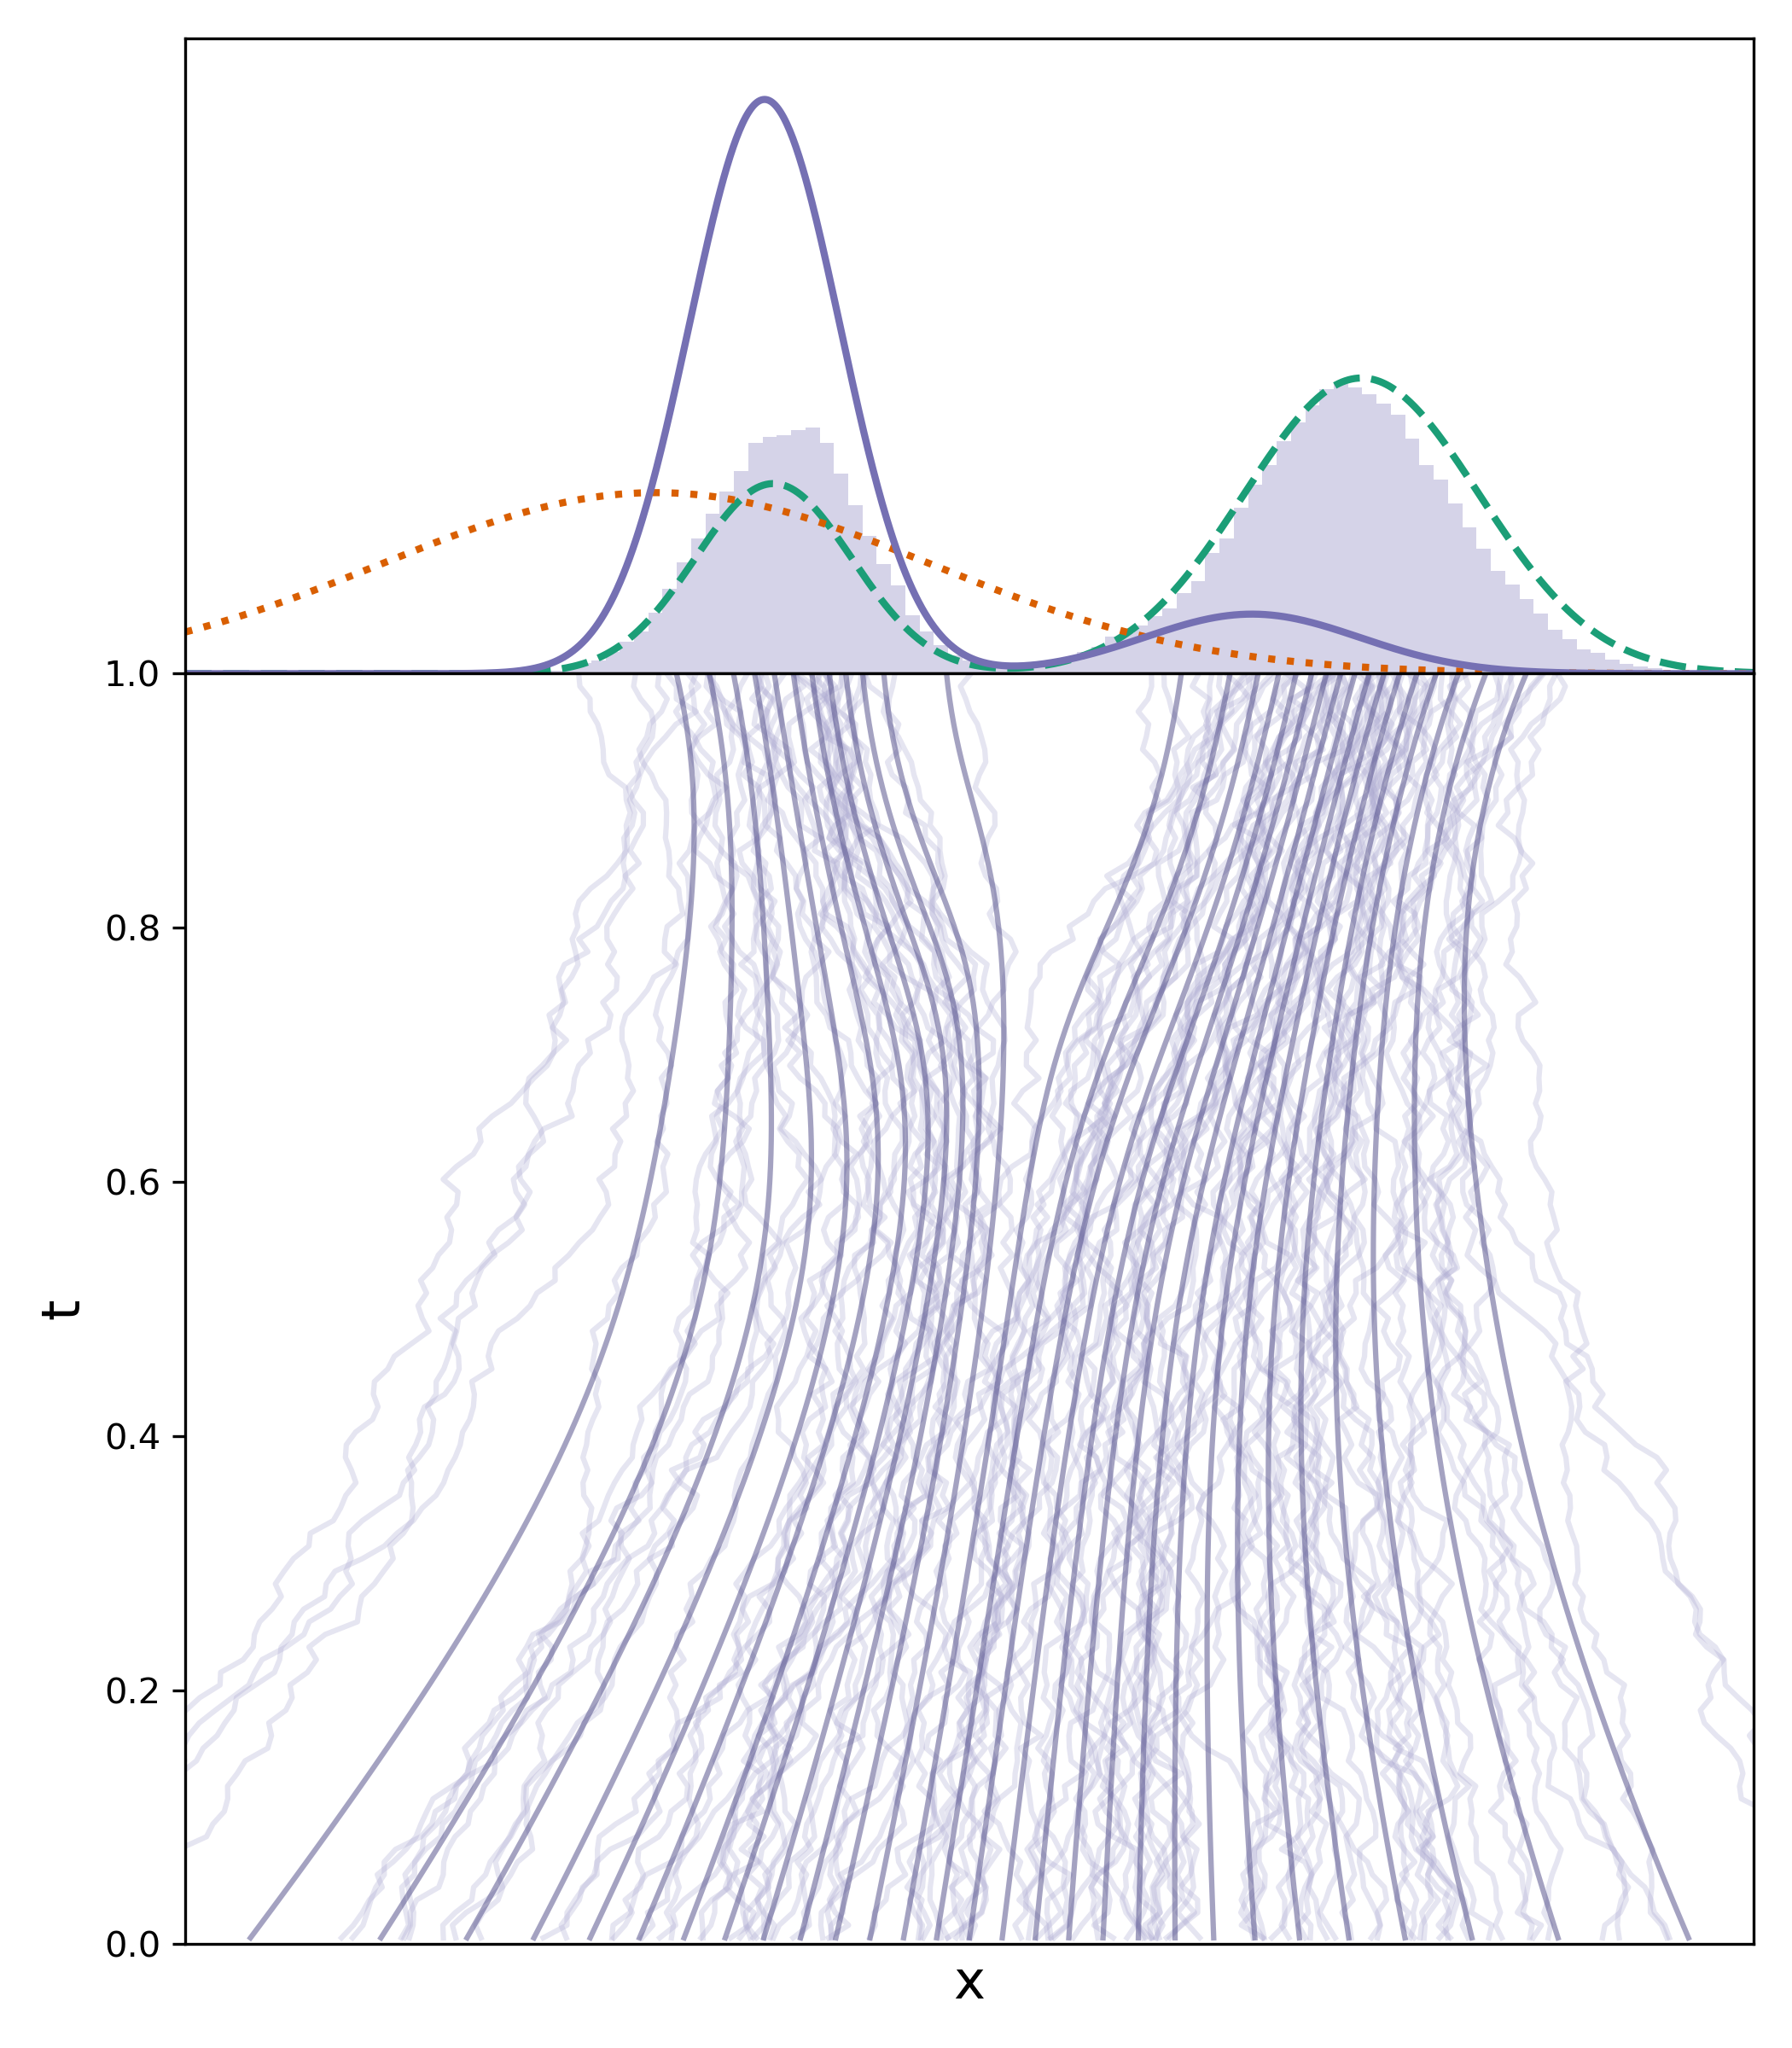
\includegraphics[width=\linewidth]{figs/finetune1d/finetuned_biased_model.png}
        \caption{Fine-tuned FM $v^\mathrm{finetune}$\\ with $\sigma(t) = 0.2$}
    \end{subfigure}%
    \begin{subfigure}[t]{0.25\linewidth}
        \centering
        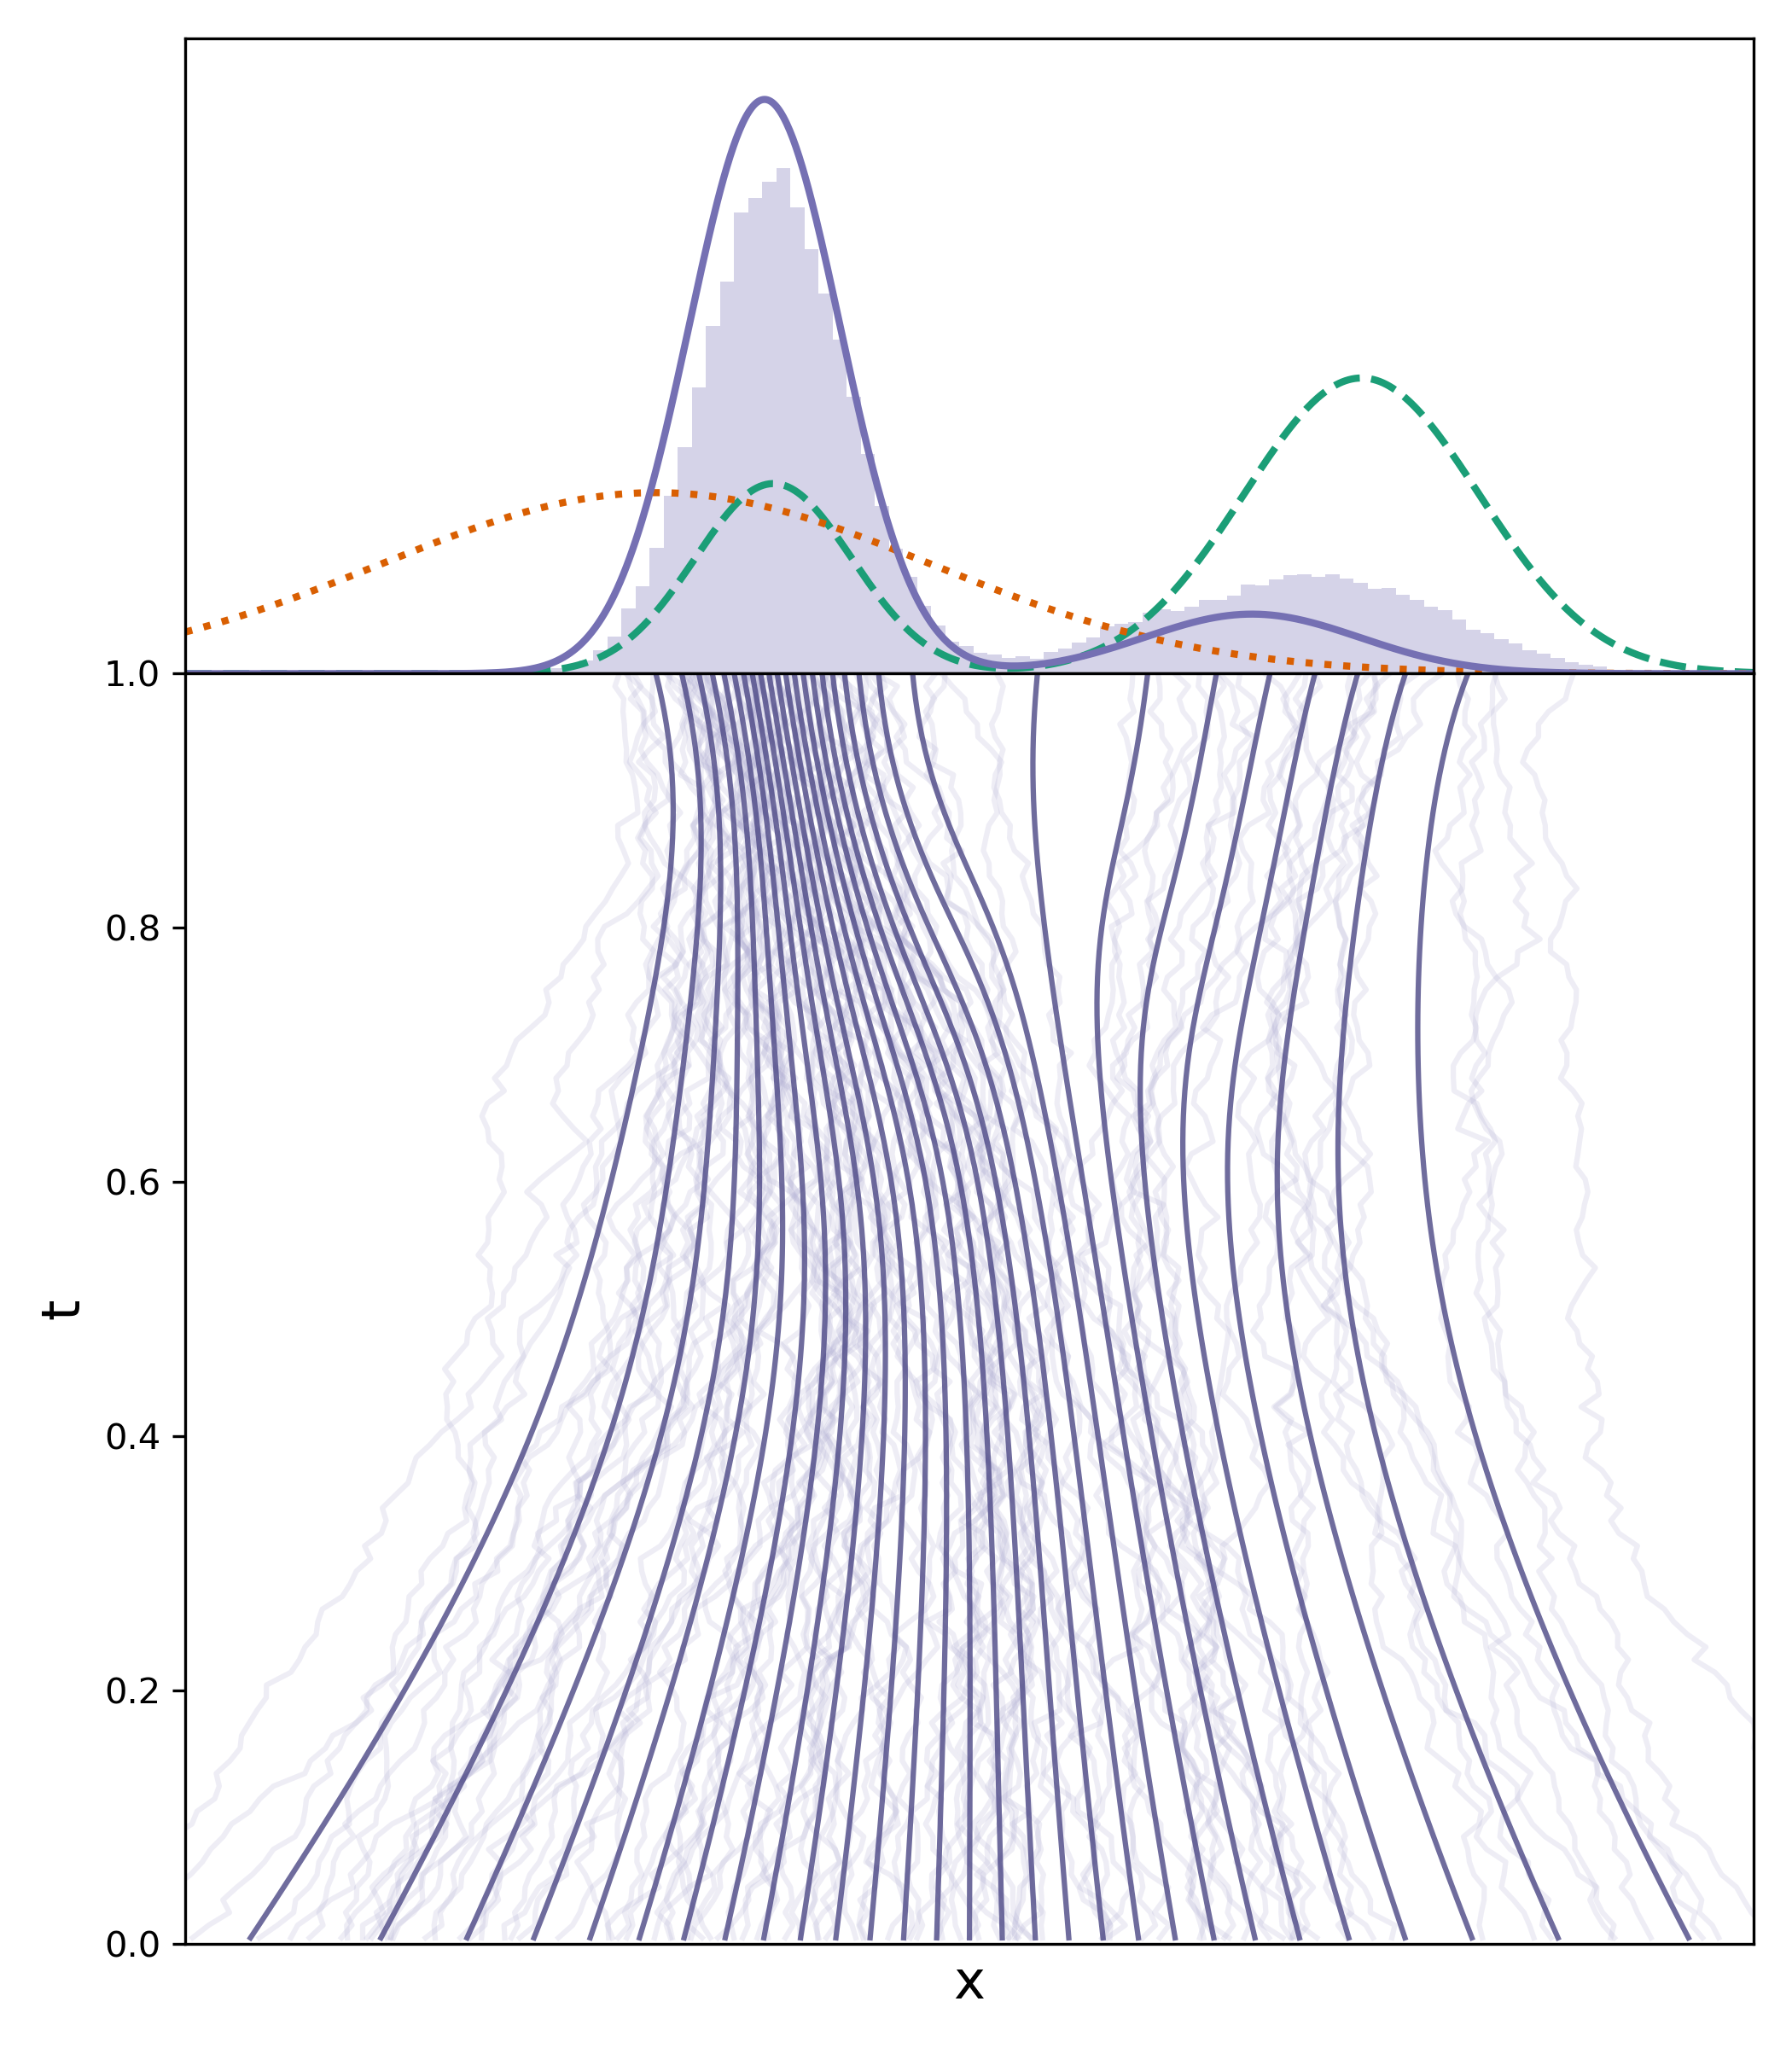
\includegraphics[width=\linewidth]{figs/finetune1d/finetuned_biased_1.0_model.png}
        \caption{Fine-tuned FM $v^\mathrm{finetune}$\\ with $\sigma(t) = 1.0$}
    \end{subfigure}%
    \begin{subfigure}[t]{0.25\linewidth}
        \centering
        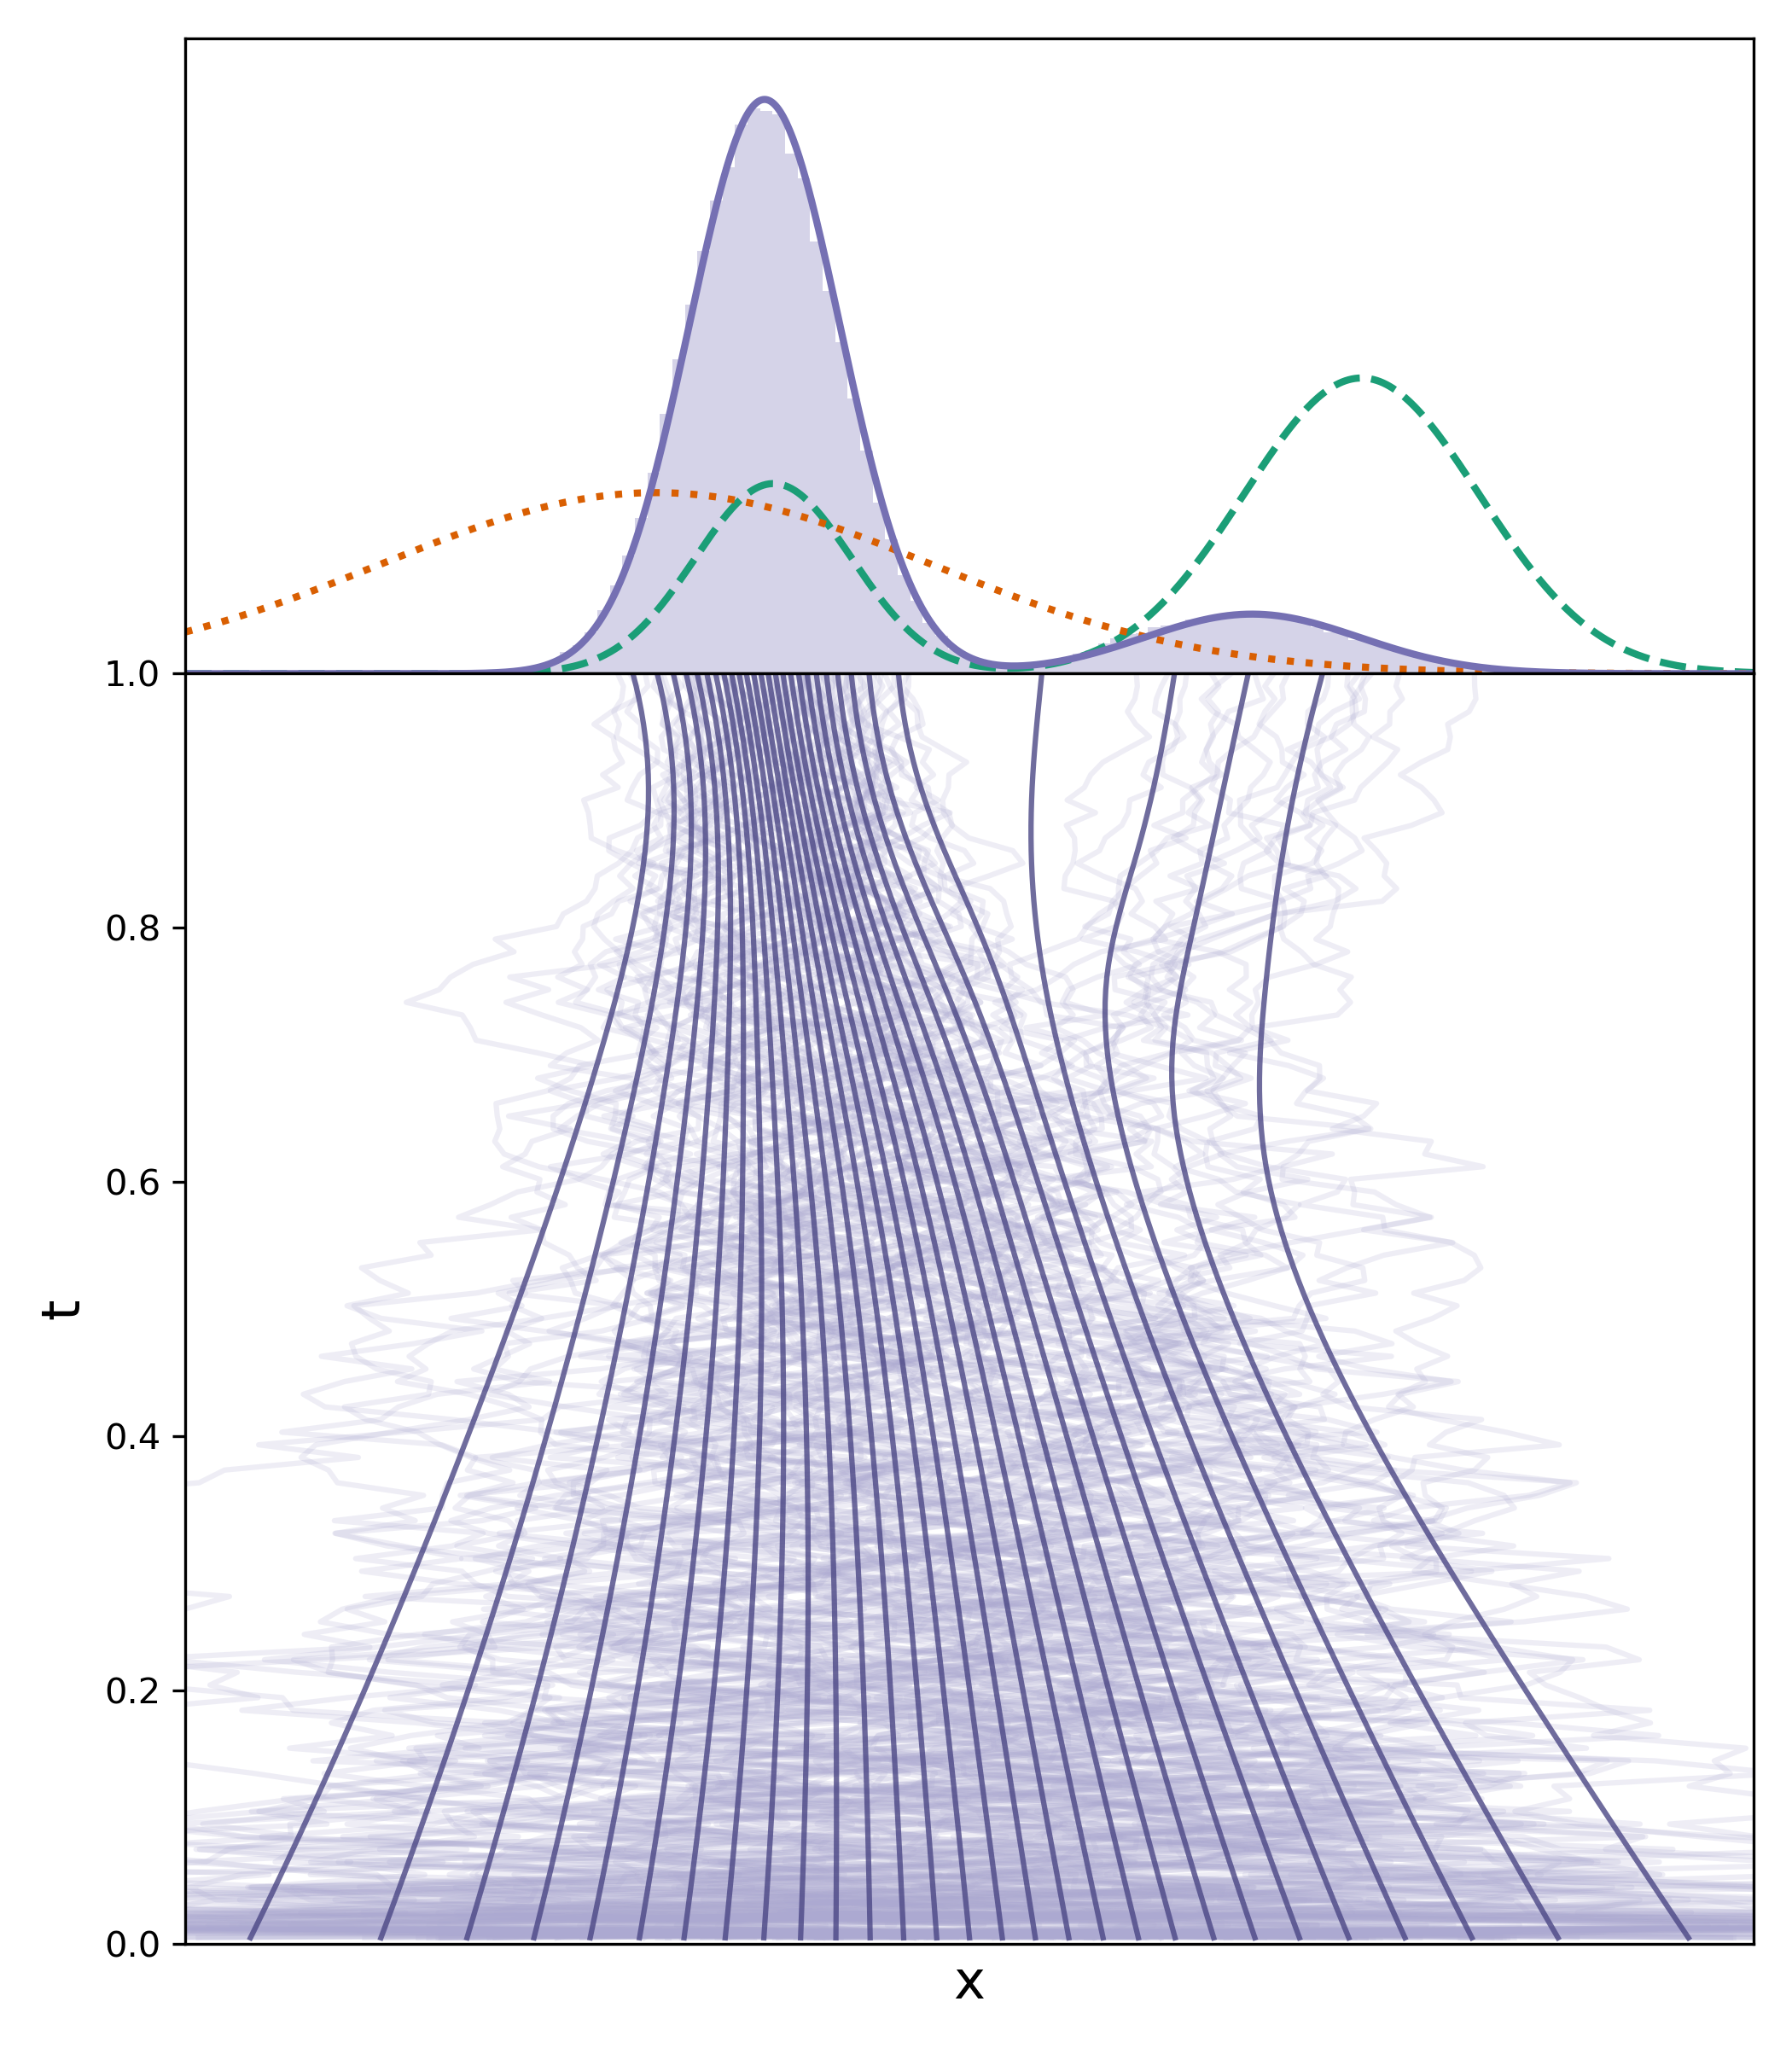
\includegraphics[width=\linewidth]{figs/finetune1d/finetuned_model.png}
        \caption{Fine-tuned FM $v^\mathrm{finetune}$\\ with memoryless $\sigma(t) = \sqrt{2\eta_t}$}
    \end{subfigure}
    \caption{Visualization of \Cref{thm:general_fine-tuning} showing that fine-tuning must be done with the memoryless noise schedule to ensure convergence to the tilted distribution \eqref{eq:p_star_info}. (a) Shows the base Flow Matching model. (b, c) Fine-tuning using a constant $\sigma(t)$ leads to biased distributions. (d) Fine-tuning using the memoryless noise schedule leads to the correct tilted distribution. Note that sample generation can use any noise schedule after fine-tuning, including $\sigma(t) = 0$.}
    \label{fig:memorylessness_illustration}
\end{figure}

For convenience, we plug the memoryless noise schedule into the controlled process for fine-tuning \eqref{eq:controlled_SDE}, and express them in terms of each respective framework.
Let $\epsilon^{\mathrm{base}}$, $v^{\mathrm{base}}$ denote the pre-trained vector fields and $\epsilon^{\mathrm{finetune}}$, $v^{\mathrm{finetune}}$ the fine-tuned vector fields. Then we have the following expressions for the full drift $b(x,t) + \sigma(t) u(x,t)$ and control $u(x,t)$ when $\sigma(t) = \sqrt{2\eta_t}$:

\quad \textit{DDIM / DDPM}:
\greybox{
\begin{talign} \label{eq:conversion_DDPM}
b(x,t) + \sigma(t) u(x,t) = \frac{\dot{\bar{\alpha}}_{t}}{2\bar{\alpha}_{t}} x - \frac{\dot{\bar{\alpha}}_{t}}{\bar{\alpha}_{t}} \frac{\epsilon^{\mathrm{finetune}}(x,t)}{\sqrt{1-\bar{\alpha}_{t}}} 
,\quad\quad
u(x,t) = 
- \sqrt{\frac{\dot{\bar{\alpha}}_t}{\bar{\alpha}_t(1-\bar{\alpha}_t)}} (\epsilon^{\mathrm{finetune}}(x,t) - \epsilon^{\mathrm{base}}(x,t)).
\end{talign}
}
\vspace{0.4em}
\quad \textit{Memoryless Flow Matching}:
\greybox{
\begin{talign} \label{eq:conversion_MFM}
b(x,t) + \sigma(t) u(x,t) = 2v^{\mathrm{finetune}}(x,t) - \frac{\dot{\alpha}_{t}}{\alpha_{t}} x 
,\quad\quad
u(x,t) = 
\sqrt{\frac{2}{\beta_{t}(\frac{\dot{\alpha}_{t}}{\alpha_{t}} \beta_{t} - \dot{\beta}_{t})}} (v^{\mathrm{finetune}}(x,t) - v^{\mathrm{base}}(x,t)).
\end{talign}
}
Thus, to solve the SOC problem \eqref{eq:control_problem_def}-\eqref{eq:controlled_SDE} in practice, we parameterize the control $u$ in terms of $\epsilon^{\mathrm{finetune}}$ or $v^{\mathrm{finetune}}$ and optimize these vector fields instead. After plugging in \eqref{eq:conversion_DDPM}-\eqref{eq:conversion_MFM}, the SOC problem \eqref{eq:control_problem_def}-\eqref{eq:controlled_SDE} can then be solved using any SOC algorithm in order to perform fine-tuning, and we proposed an especially effective algorithm next in \Cref{sec:adjoint_matching}. After fine-tuning, $\epsilon^{\mathrm{finetune}}$ and $v^{\mathrm{finetune}}$ can simply be plugged back into their respective generative processes \eqref{eq:FM_ode}-\eqref{eq:euler_maruyama_DDPM} to sample from the tilted distribution \eqref{eq:p_star_info} using any choice of diffusion coefficient. 

\section{Adjoint Matching for control-affine stochastic optimal control} \label{sec:adjoint_matching}

We discuss existing methods and also propose a new method for optimizing control-affine SOC problems. The new Adjoint Matching method is a combination of the time-tested continuous adjoint method \citep{pontryagin1962mathematical} with recent developments on constructing least-squares objectives for solving SOC problems \citep{domingoenrich2023stochastic}. In this section, we briefly discuss preliminaries on existing methods, their pros and cons, then detail the Adjoint Matching algorithm and its surprising connections to the prior methods. For numerical optimization, we now assume that the control $u$ is a parametric model with parameters $\theta$.

\subsection{Existing methods for stochastic optimal control}
\subsubsection{The adjoint method}\label{sec:adjoint_method}

The most basic method of optimizing the simulation of an SDE is to directly differentiate through the simulation using gradients from the SOC objective function \citep{han2016deep}. The adjoint method simply uses the objective:
\begin{talign} \label{eq:L_RE}
    \mathcal{L}(u ; \fX) := \int_0^1 \big(\frac{1}{2} \|u(X_t,t)\|^2 \! + \! f(X_t,t) \big) \, \mathrm{d}t \! + \! g(X_1), \qquad \fX \sim p^u.
\end{talign}
This is a stochastic estimate of the control objective in \eqref{eq:control_problem_def}, and the goal is to take compute the gradient of $\mathcal{L}(u ; \fX)$ with respect to the parameters $\theta$ of the control $u$.
Due to the continuous-time nature of SDEs, there are two main approaches to implementing this numerically. Firstly, the \emph{Discrete Adjoint} method uses a ``discretize-then-differentiate'' approach, where the numerical solver for simulating the SDE is simply stored in memory then differentiated through, and it has been studied extensively (\eg, \citet{bierkens2014explicit,gomez2014policy,hartmann2012efficient,kappen2012optimal,rawlik2013stochastic,haber2017stable}).
%The gradient of this loss with respect to the parameters $\theta$ of the control $u$ can be computed by keeping the computational graph throughout the computation of the trajectories, and then backpropagating, leveraging the power of automatic differentiation frameworks \ricky{cite}. 
This approach, however, uses an extremely large amount of memory as the full computational graph of the numerical solver must be stored in memory and implementations often must rely on gradient checkpointing \citep{chen2016training} to reduce memory usage.

Secondly, the \emph{Continuous Adjoint} method exploits the continuous-time nature of SDEs and uses an analytical expression for the gradient of the control objective with respect to the intermediate states $X_t$, expressed as an adjoint ODE, and then applies a numerical method to simulate this gradient itself, hence it is referred to as a ``differentiate-then-discretize'' approach \citep{pontryagin1962mathematical,chen2018neural,li2020scalable}. We first define the \emph{adjoint state} as: 
% the gradient of \eqref{eq:L_RE} 
% \brian{nit: $J$ is defined as the cost functional?  Is this second equality obvious / apparent?} 
% with respect to the state $X_t$:
\begin{talign}
\begin{split} \label{eq:adjoint_state_defn}
&a(t ; \fX, u) := \nabla_{X_t} 
\big(\int_t^1 \big(\frac{1}{2} \|u(X_{t'},t')\|^2 \! + \! f(X_{t'},t') \big) \, \mathrm{d}t' \! + \! g(X_1) \big), \\
&\text{where } \fX \text{ solves } \mathrm{d}X_t =  \left( b(X_t,t) + \sigma(t) u(X_t,t) \right) \, \mathrm{d}t + 
    \sigma(t) \mathrm{d}B_t.
% \\ &\text{implying }\;\; \mathbb{E}_{\fX \sim p^u} \left[ a(t ; \fX, u) \;|\; X_t = x \right] = \nabla_{x} J(u; x, t),
\end{split}
\end{talign}
This implies that $\mathbb{E}_{\fX \sim p^u} \left[ a(t ; \fX, u) \;|\; X_t = x \right] = \nabla_{x} J(u; x, t)$,
where $J$ denotes the cost functional defined in \eqref{eq:cost_functional}.
It can then be shown that this adjoint state satisfies 
% \brian{Will we show this in an appendix?}\ricky{TODO: appendix}%
\footnote{Note we use the convention that a Jacobian matrix $J = \nabla_x v(x)$ is defined as $J_{ij} = \frac{\partial v_i(x)}{\partial x_j}$.}%
:
\begin{talign} 
\begin{split} \label{eq:cont_adjoint_1}
    \frac{\mathrm{d}}{\mathrm{d}t} a(t;\fX,u)  &=  - \left[ a(t;\fX,u)\tran{} \left(\nabla_{X_t} (b (X_t,t) + \sigma(t) u(X_t,t))\right) 
    + \nabla_{X_t} \left( f(X_t,t) + \frac{1}{2}\|u(X_t,t)\|^2 \right) \right],
\end{split}
    \\ a(1;\fX,u) &= \nabla g(X_1). \label{eq:cont_adjoint_2}
\end{talign}
The adjoint state is solved backwards in time, starting from the terminal condition \eqref{eq:cont_adjoint_2}. Computation of \eqref{eq:cont_adjoint_1} can be efficiently done as a vector-Jacobian product on automatic differentiation software \citep{paszke2019pytorch}. Once the adjoint state has been solved for $t \in [0, 1]$, then the gradient of $\mathcal{L}(u ; \fX)$ with respect to the parameters $\theta$ can be obtained by integrating over the entire time interval: 
% \brian{Is this obvious / apparent?}
\begin{talign}\label{eq:continuous_adjoint_grads}
    \frac{\mathrm{d} \mathcal{L}}{\mathrm{d} \theta} =  
    \frac{1}{2}\int_0^1 \frac{\partial}{\partial \theta} \norm{u(X_t, t)}^2 \mathrm{d} t
    +\int_0^1 \frac{\partial u(X_t, t)}{\partial \theta}\tran{} \sigma(t)\tran{} a(t; \fX, u) \mathrm{d} t,
\end{talign}
where the first term is the partial derivative of $\mathcal{L}$ w.r.t. $\theta$ and the second term is the partial derivative through the sample trajectory $\fX$. See \Cref{prop:cont_adjoint_method} in \Cref{subsec:derivation_cont_adj_method} for a statement and proof of this result. 
The discrete and continuous adjoint methods converge to the same gradient as the step size of the numerical solvers go to zero. 
Both are scalable to high dimensions and have seen their fair share of usage in optimizing neural ODE/SDEs \citep{chen2018neural,chen2021learning,li2020scalable}. As the adjoint methods are essentially gradient-based optimization algorithms applied on a highly non-convex problem, many have also reported they can be unstable empirically \citep{mohamed2020monte,suh2022differentiable,domingoenrich2023stochastic}.

\subsubsection{Importance-weighted matching objectives for regressing onto the optimal control}
\label{sec:socm}

An alternative is to consider regressing onto the optimal control $u^*$, which is the approach of the cross-entropy method~\citep{rubinstein2013cross,zhang2014applications} and stochastic optimal control matching (SOCM; \citet{domingoenrich2023stochastic}). These methods make use of path integral theory \citep{kappen2005path} to express the optimal control through importance sampling, resulting in an \emph{importance-weighted} least-squares objective function
\begin{talign}\label{eq:socm_objective}
    \mathcal{L}_{\text{SOCM}}(u; \fX) := \int_0^1 \norm{u(X_t, t) - \hat{u}^*(X_t, t)}^2 \mathrm{d} t \times \omega(u, \fX), \qquad \fX \sim p^u,
\end{talign}
where $\omega$ is an importance weighting that approximates sampling from the optimal distribution $p^*$, and $\hat{u}^*$ is a stochastic estimator of the optimal control relying on having sampled from the optimal process. We defer to \citet{domingoenrich2023stochastic} for the exact details. The functional landscape of this objective is convex, which is argued to help yield stable training. However, the need for importance sampling renders this impractical for high dimensional applications: the variance of the importance weighting $\omega$ grows exponentially with dimension of the stochastic process, leading to catastrophic failure. This unfortunately means that such importance-weighted matching objectives are impractical for fine-tuning dynamical generative models; however, a least-squares objective is greatly coveted as it can lead to stable training and simple interpretations.

\subsection{Adjoint Matching} \label{subsec:adjoint_matching}

We make two important observations which lead to our proposed method: (\textit{i}) it is possible to construct a matching objective without any importance weighting, and (\textit{ii}) there are unnecessary terms in the adjoint differential equation \eqref{eq:cont_adjoint_1} that can lead to higher variance at convergence.

Firstly, we notice that we can simply match the gradient of the cost functional under the \textit{current} control. That is, while SOCM carefully constructs an importance-weighted estimator of the \textit{optimal} control $u^* = - \sigma(t)\tran{} \nabla J(u^*; x, t)$ \eqref{eq:optimal_control}, we claim that we can actually just regress onto the target vector field $- \sigma(t)\tran{} \nabla J(u; x, t)$ where $u$ is the current control, and furthermore, this results in a gradient equal in expectation to the continuous adjoint method. 
%
We formalize this in the following proposition, proven in \Cref{subsec:derivation_continuous}: 
\begin{proposition} \label{prop:continuous_adjoint_loss_main}
    Let us define, for now, the basic Adjoint Matching objective as:
    \begin{talign}
    \begin{split} \label{eq:cont_adjoint}
        \mathcal{L}_{\mathrm{Basic-Adj-Match}}(u; \fX) &:= \frac{1}{2} \int_0^{1} \big\| u(X_t,t)
        + \sigma(t)\tran{} a(t;\bm{X},\bar{u}) \big\|^2 \, \mathrm{d}t, \qquad \fX \sim p^{\bar{u}}, \quad \bar{u} = \texttt{stopgrad}(u),
    \end{split}
    \end{talign}
    where $\bar{u} = \texttt{stopgrad}(u)$ means that the gradients of $\bar{u}$ with respect to the parameters $\theta$ of the control $u$ are artificially set to zero. The gradient of $\mathcal{L}_{\mathrm{Basic-Adj-Match}}(u; \fX)$ with respect to $\theta$ is equal to the gradient $\frac{\mathrm{d} \mathcal{L}}{\mathrm{d} \theta}$ in equation \eqref{eq:continuous_adjoint_grads}.
    Importantly, the only critical point of $\E \left[\mathcal{L}_{\mathrm{Basic-Adj-Match}} \right]$ is the optimal control $u^*$.
\end{proposition}

Critical points of $\mathcal{L}$ are controls $u$ such that $\frac{\delta}{\delta u} \mathcal{L}(u) = 0$, where $\frac{\delta}{\delta u} \mathcal{L}$ denotes the first variation of the functional $\mathcal{L}$.
In other words, \Cref{prop:continuous_adjoint_loss_main} states that the only control that satisfies the first-order optimality condition for the basic Adjoint Matching objective is the optimal control, which provides theoretical grounding for gradient-based optimization algorithms. 

An intuitive way to understand the basic Adjoint Matching objective is that it is a \emph{consistency loss}. The Adjoint Matching objective is based off of the observation that the optimal control $u^*(x, t)$ is the unique fixed-point of the relation $u(x,t) = -\sigma(t)\tran{} \nabla_x J(u; x, t)$ (see \Cref{eq:lemma_cost_functional} in \Cref{subsec:derivation_continuous})
%\brian{Citation?  Is this obvious?  Or part of the proof of proposition 2?}, 
and so we are directly optimizing for a control that fits this relation, while using the adjoint state as a stochastic estimator of $\nabla_x J(u; x, t)$ \eqref{eq:adjoint_state_defn}. 
% This uniqueness property has previously been used to justify the adjoint method by showing that the optimal control is the unique critical point of the adjoint method \ricky{cite}; however, to the best of our knowledge, it has not been used to directly construct a consistency loss like the basic Adjoint Matching objective.

The basic Adjoint Matching objective in \Cref{prop:continuous_adjoint_loss_main} does not yet yield a novel algorithm for stochastic optimal control, because it produces the same gradient as the continuous adjoint method. This can be seen by taking the gradient w.r.t. $\theta$ after expanding the square in \eqref{eq:cont_adjoint} and removing terms that do not depend on $\theta$ to arrive exactly at the continuous adjoint method~\eqref{eq:continuous_adjoint_grads}. 
However, it provides the means of deriving a simpler \textit{leaner} objective function.

\paragraph{The ``Lean'' Adjoint.} The minimizer of a least-squares objective is the conditional expectation of the regression target, so for the Adjoint Matching objective, at the optimum we have that
\begin{talign}
    u^*(x, t) = \E_{\fX \sim p^*} \left[ -\sigma(t)\tran{} a(t; \fX, u^*) | X_t = x\right].
\end{talign}
Multiplying both sides by the Jacobian $\nabla_x u^*(x, t)$ and re-arranging, we get the relation
\begin{talign}\label{eq:cancellation_terms}
    \E_{\fX \sim p^*} \left[ u^*(x, t)\tran{} \nabla_x u^*(x, t) + a(t; \fX, u^*) \tran{} \sigma(t) \nabla_x u^*(x, t) \;|\; X_t = x\right] = 0.
\end{talign}
Notice that the terms inside the expectation in \eqref{eq:cancellation_terms} show up as part of the adjoint differential equation \eqref{eq:cont_adjoint_1}, which we have now shown to have expectation zero at the optimal solution. 
% Furthermore, the variance of the terms inside \eqref{eq:cancellation_terms} is non-zero even at the optimal solution, so the basic Adjoint Matching \eqref{eq:cont_adjoint} and hence \emph{the continuous adjoint method will also have non-vanishing gradients even when $u=u^*$}.
Therefore, we motivate the definition of a \emph{lean adjoint state} $\tilde{a}$ with the terms in \eqref{eq:cancellation_terms} removed. Plugging this lean adjoint back into the least-squares objective, we obtain our final proposed Adjoint Matching objective: 
\graybox{
\begin{talign}\label{eq:lean_adjoint_matching}
\mathcal{L}_{\mathrm{Adj-Match}}(u; \fX) 
:= \frac{1}{2} \int_0^{1} \big\| & u(X_t %^{\bar{u}}
,t)
+ \sigma(t)\tran{} \tilde{a}(t;\bm{X} %^{\bar{u}}
) \big\|^2 \, \mathrm{d}t, 
\qquad \fX \sim p^{\bar{u}}, \quad \bar{u} = \texttt{stopgrad}(u), \\
%
\label{eq:lean_adjoint_1}
\text{where }\quad \frac{\mathrm{d}}{\mathrm{d}t} \tilde{a}(t;\bm{X}) 
&= - (\tilde{a}(t;\bm{X})^{\top} \nabla_x b (X_t,t) + \nabla_x f(X_t,t)), \\ 
%
\label{eq:lean_adjoint_2}
\tilde{a}(1;\bm{X}) &= \nabla_x g(X_1).
\end{talign}
}
Equations \eqref{eq:lean_adjoint_1}-\eqref{eq:lean_adjoint_2} define the \emph{lean adjoint state}, and \eqref{eq:lean_adjoint_matching} is the complete Adjoint Matching objective.
\textit{The unique critical point of $\mathbb{E}[\mathcal{L}_{\mathrm{Adj-Match}}]$ is the optimal control}, which we prove relying on \Cref{prop:continuous_adjoint_loss_main} and equation \eqref{eq:cancellation_terms} (see \Cref{prop:lean_adjoint} in \Cref{subsec:proof_lean_adjoint}). 

Compared to the importance sampling methods (\Cref{sec:socm}), Adjoint Matching is a simple least-squares regression objective and has no importance weighting. This allows it to avoid the pitfalls of high variance importance weights and makes it as scalable as the adjoint methods while retaining the interpretation of matching a target vector field.

Compared to the adjoint method (\Cref{sec:adjoint_method}), Adjoint Matching produces a \emph{different gradient in expectation than the continuous adjoint}. This is because the lean adjoint state is not related to the gradient of the cost functional anymore, \ie, \eqref{eq:adjoint_state_defn} is not true, except at the optimum when $u=u^*$.
Even at the optimal solution, since Adjoint Matching removes terms that have expectation zero, it can potentially exhibit better convergence and lower variance than the continuous adjoint method. 
Additionally, computation of the lean adjoint state \eqref{eq:lean_adjoint_1} also exhibits a smaller computational cost due to the removal of the extra terms (no longer need the Jacobian of the control $\nabla_x u$).
We provide a rigorous derivation of Adjoint Matching and the above claims in \Cref{subsec:proof_lean_adjoint}.

Adjoint Matching can be applied to reward fine-tuning of dynamical generative models through the memoryless SOC formulation discussed in \Cref{sec:memoryless_SOC}. We provide pseudo-code for this in \Cref{alg:adjoint_matching_finetuning_FM} for Flow Matching models and in \Cref{alg:adjoint_matching_finetuning_DDIM} in \Cref{subsec:pseudocode_DDIM} for denoising diffusion models.

% \begin{algorithm}
% \SetAlgoNoLine % Disable line numbering
% \SetAlgoNlRelativeSize{0} %Set number line font to zero
% \small{
% \KwIn{Pre-trained FM velocity field $v^{\mathrm{base}}$ or noise predictor $\epsilon^{\mathrm{base}}$, number of fine-tuning iterations $N$.}

% Initialize fine-tuned vector fields: $v^{\mathrm{finetune}} = v^{\mathrm{base}}$ or $\epsilon^{\mathrm{finetune}} = \epsilon^{\mathrm{base}}$ with parameters $\theta$.

%   \For{$n \in \{0,\dots,N-1\}$}{
%     Sample $m$ trajectories $\bm{X} = (X_k)_{k\in\{0,\dots, K\}}$ with memoryless noise schedule (\Cref{prop:memorylessness_noise_schedule}), \eg using:
%     \begin{itemize}
%     \item the FM update \eqref{eq:FM_discretizatio} with $v = v^{\mathrm{finetune}}$ and $\sigma_k = \sqrt{2\beta_{k}(\frac{\alpha_{k+1} - \alpha_k}{\alpha_{k}} \beta_{k} - \beta_{k+1} + \beta_{k})}$, 
%     \item or the DDIM update \eqref{eq:DDIM_original_main} with $\epsilon = \epsilon^{\mathrm{finetune}}$ and $\sigma_k = \sqrt{\frac{\bar{\alpha}_{k+1} - \bar{\alpha}_{k}}{\bar{\alpha}_{k}}}$.
%     \end{itemize}

%     For each trajectory, solve the \textit{lean adjoint ODE} \eqref{eq:lean_adjoint_1}-\eqref{eq:lean_adjoint_2} backwards in time from $k={K}$ to $1$:
%     \begin{talign}
%         \tilde{a}_{k-1} 
%         &= \tilde{a}_{k} + \frac{1}{K} \tilde{a}_k\tran{} \nabla_{X_k} b_k (X_k), \qquad 
%         \tilde{a}_K = \nabla_{X_K} r(X_K), \qquad \text{where} \\
%         b_k(x) &=
%         \begin{cases}
%             2 v^\text{base}(x,\frac{k}{K}) - \frac{\alpha_{k+1} - \alpha_k}{K\alpha_{k}} x & \text{for FM} \\
%             \frac{\bar{\alpha}_{k+1} - \bar{\alpha}_{k}}{2\bar{\alpha}_{k}} x - \frac{\bar{\alpha}_{k+1} - \bar{\alpha}_k}{\bar{\alpha}_{k} \sqrt{1-\bar{\alpha}_{k}}}\epsilon^{\mathrm{base}}(x,k) & \text{for DDIM}.
%         \end{cases}
%     \end{talign}

%     Note that $X_k$ and $\tilde{a}_k$ should be computed without gradients, \ie, $X_k = \texttt{stopgrad}(X_k)$, $\tilde{a}_k = \texttt{stopgrad}(\tilde{a}_k)$. \vspace{0.5em}

%     For each trajectory, compute the Adjoint Matching objective \eqref{eq:lean_adjoint_matching}: 
%     \begin{talign}
%     \mathcal{L}_{\mathrm{Adj-Match}}(\theta) = 
%     \begin{cases}
%         \frac{1}{K} \sum_{k=0}^{K-1} \big\|\frac{2}{\sigma_k} \big(v^{\mathrm{finetune}}_{\theta}(X_k,\frac{k}{K}) - v^{\mathrm{base}}(X_k,\frac{k}{K}) \big) + \sigma_k \tilde{a}_{k} \big\|^2 & \text{for FM} \\
%         \frac{1}{K} \sum_{k=0}^{K-1} \| - \frac{\bar{\alpha}_{k+1} - \bar{\alpha}_k}{\sigma_k \bar{\alpha}_{k} \sqrt{1-\bar{\alpha}_{k}}} \big( \epsilon^{\mathrm{finetune}}_{\theta}(X_k,k) - \epsilon^{\mathrm{base}}(X_k,k) \big) + \sigma_k \tilde{a}_{k} \|^2 & \text{for DDIM}
%     \end{cases}
%     \end{talign}

%     Compute the gradient $\nabla_{\theta} \mathcal{L}(\theta)$ and update $\theta$ using favorite gradient descent algorithm.
%   }
% \KwOut{Fine-tuned vector field $v^{\mathrm{finetune}}$ or $\epsilon^{\mathrm{finetune}}$}}
% \caption{Adjoint Matching for Fine-tuning Flow Matching and Diffusion Models}
% \label{alg:adjoint_matching_finetuning}
% \end{algorithm}

\begin{algorithm}
\SetAlgoNoLine % Disable line numbering
\SetAlgoNlRelativeSize{0} %Set number line font to zero
\small{
\KwIn{Pre-trained FM velocity field $v^{\mathrm{base}}$, step size $h$, number of fine-tuning iterations $N$.}

Initialize fine-tuned vector fields: $v^{\mathrm{finetune}} = v^{\mathrm{base}}$ with parameters $\theta$.

  \For{$n \in \{0,\dots,N-1\}$}{
    Sample $m$ trajectories $\bm{X} = (X_t)_{t\in\{0, \dots, 1\}}$ with memoryless noise schedule $\sigma(t) = \sqrt{2 \beta_t (\frac{\dot{\alpha}_t}{\alpha_t} \beta_t - \dot{\beta}_t)}$, \eg :
    \begin{talign} \label{eq:EM_update_box}
    X_{t+h} = X_{t} + h \left(2v_\theta^{\mathrm{finetune}}(X_t, t) - \frac{\dot{\alpha}_t}{\alpha_t} X_t \right) + \sqrt{h} \sigma(t) \varepsilon_t, \quad\quad \varepsilon_t \sim \mathcal{N}(0, I), \quad\quad X_0 \sim \mathcal{N}(0, I).
    \end{talign}

    For each trajectory, solve the \textit{lean adjoint ODE} \eqref{eq:lean_adjoint_1}-\eqref{eq:lean_adjoint_2} backwards in time from $t={1}$ to $0$, \eg:
    \begin{talign} \label{eq:Euler_lean_adjoint}
        \tilde{a}_{t-h} 
        = \tilde{a}_{t} + h \tilde{a}_t\tran{} \nabla_{X_t} \left(2v^{\mathrm{base}}(X_t, t) - \frac{\dot{\alpha}_t}{\alpha_t} X_t \right), \qquad 
        \tilde{a}_1 = - \nabla_{X_1} r(X_1).
    \end{talign}

    Note that $X_t$ and $\tilde{a}_t$ should be computed without gradients, \ie, $X_t = \texttt{stopgrad}(X_t)$, $\tilde{a}_t = \texttt{stopgrad}(\tilde{a}_t)$. \vspace{0.5em}

    For each trajectory, compute the Adjoint Matching objective \eqref{eq:lean_adjoint_matching}: 
    \begin{talign} \label{eq:adj_matching_algorithm_box}
    \mathcal{L}_{\mathrm{Adj-Match}}(\theta) =
        \sum_{t\in\{0, \dots, 1 - h\}} \big\|\frac{2}{\sigma(t)} \big(v^{\mathrm{finetune}}_{\theta}(X_t, t) - v^{\mathrm{base}}(X_t, t) \big) + \sigma(t) \tilde{a}_t \big\|^2.
    \end{talign}

    Compute the gradient $\nabla_{\theta} \mathcal{L}(\theta)$ and update $\theta$ using favorite gradient descent algorithm.
  }
\KwOut{Fine-tuned vector field $v^{\mathrm{finetune}}$}}
\caption{Adjoint Matching for fine-tuning Flow Matching models}
\label{alg:adjoint_matching_finetuning_FM}
\end{algorithm}

\section{Related work} 

\paragraph{Fine-tuning from human feedback.}
There are two main overarching approaches to RLHF: the \textit{reward-based} approach \citep{ziegler2020finetuning,stiennon2020learning,ouyang2022training,bai2022training} and \textit{direct preference optimization} (DPO; \cite{rafailov2023direct}).
The reward-based approach \citep{ziegler2020finetuning,stiennon2020learning,ouyang2022training,bai2022training} consists in learning the reward model $r(x)$ from human preference data, and then solving a maximum entropy RL problem with rewards produced by $r(x)$. 
DPO merges the two previous steps into one: there is no need to learn $r(x)$ as human preference data is directly used to fine-tune the model. 
However, DPO is typically only applied with a filtered dataset, and does not work explicitly with a reward model.
Furthermore, for flow and diffusion models specifically, it is possible to differentiate the reward function, so there is a larger emphasis on reward-based approaches.

\paragraph{Fine-tuning for diffusion models.}
Among existing reward-based diffusion fine-tuning methods, \citet{fan2023optimizing} interpret the denoising process as a multi-step decision-making task and use policy gradient algorithms to fine-tune diffusion samplers. 
%They restrict their attention to rewards that are integral probability metrics between a target distribution and the generated distribution. 
\citet{black2024training} makes use of proximal policy gradients for fine-tuning but this does not make use of the differentiability of the reward model. 
\citet{fan2023dpok} also consider KL-regularized rewards \eqref{eq:kl_regularized_interpretation} but do not make the critical connection to the tilted distribution \eqref{eq:p_star_info} that we flesh out in \Cref{sec:value_function_bias_problem}. 
The fine-tuning algorithms of \cite{xu2023imagereward,clark2024directly} directly take gradients of the reward model and use heuristics to try to stay close to the original base generative model, but their behavior is not well understood and unrelated to the tilted distribution: \cite{xu2023imagereward} takes gradients of the reward applied on the denoised sample at different points in time, and \cite{clark2024directly} backpropagates the reward function through all or part of the diffusion trajectory. 
Finally, \cite{uehara2024finetuning} also fine-tune diffusion models with the goal of sampling from the tilted distribution \eqref{eq:p_star_info}, but their approach is much more involved than ours as it requires learning a value function, and solving two stochastic optimal control problems. Additional reward fine-tuning works include \cite{bruna2024posterior}, that provide theoretical guarantees to sample from the tilted distribution when the reward is a quadratic function, and \cite{zhang2024improving}, that propose a reward fine-tuning algorithm for the GFlowNet architecture. 

\paragraph{Inference-time optimization methods.} Some have proposed methods that do not update the base model but instead modify the generation process directly. One approach is to add a guidance term to the velocity \citep{chung2022diffusion,song2023pseudoinverse,pokle2023training}; however, this is a heuristic and it is not well-understood what particular distribution is being generated. Another approach is to directly optimize the initial noise distribution \citep{li2021differentiable,wallace2023endtoend,benhamu2024dflow}; this is taking an opposite approach to the inital value bias problem than us by moving all of the work into optimizing the initial distribution. 
A more computationally intensive approach is to perform online estimation of the optimal control, for the purpose of heuristically solving an optimal control problem within the sampling process~\citep{huang2024symbolic,rout2024rb}; these approaches aim to solve a separate control problem for each generated sample, instead of performing amortization \citep{amos2023tutorial} to learn a fine-tuned generative model.

\paragraph{Optimal control in generative modeling.} Methods from optimal control have been used to train dynamical generative models parameterized by ODEs \citep{chen2018neural}, SDEs \citep{li2020scalable}, and jump processes \citep{chen2021learning}, enabled through the adjoint method. 
They can be used to train arbitrary generative processes, but for simplified constructions these have fallen in favor of simulation-free matching objectives such as denoising score matching \citep{vincent2011connection} and Flow Matching \citep{lipman2023flow}. 
The optimal control formalism also has significance in sampling from un-normalized distributions \citep{zhang2022path,berner2023optimal,vargas2023denoising,vargas2022bayesian,richter2024improved,tzen2019theoretical}. 
The inclusion of a state cost has been used to solve transport problems where intermediate path distributions are of importance \citep{liu2023generalized,pooladian2024neural}.
These collective advances naturally lead to the consideration of the optimal control formalism for reward fine-tuning.

\paragraph{Conditional sampling in inverse problems.} \cite{denker2024deft} and \cite{wu2023practical} independently consider a pre-trained diffusion model $p(x)$, and an observation $y$ on the generated sample $x$, as well as the analytic likelihood $p(y|x)$. Their aim is to sample from the posterior $p(x) p(y|x)$, and their applications include inpainting, class-conditional generation, super-resolution, phase retrieval, non-linear deblurring, computed tomography, and protein design. Their setting reduces to a particular case of our reward fine-tuning framework by setting $r(x) = \log p(y|x)$. \cite{denker2024deft} formulate an SOC problem, and they solve it via the log-variance loss (\cite{richter2020vargrad,nüsken2023solving}), and the moment loss \citep{nüsken2023solving}\footnote{See also \cite{domingoenrich2024taxonomy} for a comparison among SOC losses.}, which they refer to as the trajectory balance loss \citep{malkin2023trajectory}. \cite{wu2023practical} propose Twisted Diffusion Sampler, an algorithm based on Sequential Monte Carlo that uses increased inference-time compute to reduce bias.
%can be understood as a poor man's SOC solver combined with importance reweighting to reduce the bias introduced by the suboptimal control. 
A third work that also tackles the conditional sampling problem is \cite{du2024doobs}, which use a Lagrangian formulation that they solve approximately using Gaussian paths. 

\section{Experiments} \label{sec:diff_finetuning_exp}

\begin{table}[t]
\centering
% \resizebox{\textwidth}{!}{%
\small
\begin{tabular}{llccccccc}
    \toprule
    & Fine-tuning & Fine-tuning & Sampling & \multirow{2}{*}{ClipScore$\, \uparrow$} & \multirow{2}{*}{PickScore$\, \uparrow$} & \multirow{2}{*}{HPS v2$\, \uparrow$} & DreamSim 
    % & Total time (s) / 
    \\
    & Method & $\sigma(t)$ & $\sigma(t)$ &  &  &  & Diversity$\, \uparrow$ 
    % & \# iterations 
    \\
    \midrule
    & None & \multirow{2}{*}{\color{gray}N/A} & $\sqrt{2 \eta_t}$ & 24.15{\tiny$\pm$0.26} & 17.25{\tiny$\pm$0.06} & 16.19{\tiny$\pm$0.17} & 53.60{\tiny$\pm$1.37} 
    % & \multirow{2}{*}{\color{gray}N/A} 
    \\ 
    & (Base model)
                                 &                     & 0                 & 28.32{\tiny$\pm$0.22} & 18.15{\tiny$\pm$0.07} & 17.89{\tiny$\pm$0.16} & \textbf{56.53{\tiny$\pm$1.52}} 
                                 % &  
                                 \\
    \midrule % \addlinespace
    \parbox[t]{2mm}{\multirow{8}{*}{\rotatebox[origin=c]{90}{Baselines \;\;\;}}}
    & \multirow{2}{*}{DRaFT-1}           & $\sqrt{2 \eta_t}$ & $\sqrt{2 \eta_t}$ & 30.18{\tiny$\pm$0.24} & 19.38{\tiny$\pm$0.08} & 24.61{\tiny$\pm$0.17} & 25.54{\tiny$\pm$0.99} 
    % & 140k{\tiny$\pm$5.9k} 
    \\
    &                                   & 0                 & 0                 & 30.95{\tiny$\pm$0.28} & 19.37{\tiny$\pm$0.06} & 24.37{\tiny$\pm$0.17} & 27.39{\tiny$\pm$1.14} 
    % & / 4000 
    \\
    \addlinespace
    & \multirow{2}{*}{DRaFT-40}          & $\sqrt{2 \eta_t}$ & $\sqrt{2 \eta_t}$ & 26.94{\tiny$\pm$0.28} & 18.34{\tiny$\pm$0.19} & 19.98{\tiny$\pm$1.02} & 41.98{\tiny$\pm$2.14} 
    % & 148k{\tiny$\pm$4.2k} 
    \\
    &                                   & 0                 & 0                 & 30.07{\tiny$\pm$0.39} & 19.45{\tiny$\pm$0.08} & 24.06{\tiny$\pm$0.24} & 36.53{\tiny$\pm$1.69} 
    % & / 1500 
    \\
    \addlinespace
    & \multirow{2}{*}{DPO}          & $\sqrt{2 \eta_t}$ & $\sqrt{2 \eta_t}$ & 24.11{\tiny$\pm$0.22} & 17.24{\tiny$\pm$0.06} & 16.15{\tiny$\pm$0.14} & 53.27{\tiny$\pm$1.36} 
    % & 118k{\tiny$\pm$0.6k} 
    \\
    &                                   & 0                 & 0                 & 27.77{\tiny$\pm$0.18} & 17.92{\tiny$\pm$0.07} & 17.30{\tiny$\pm$0.20} & 54.11{\tiny$\pm$1.50} 
    % & / 1000 
    \\
    \addlinespace
    & \multirow{2}{*}{ReFL}              & $\sqrt{2 \eta_t}$ & $\sqrt{2 \eta_t}$ & 28.59{\tiny$\pm$0.31} & 18.68{\tiny$\pm$0.10} & 22.24{\tiny$\pm$0.46} & 32.71{\tiny$\pm$2.76} 
    % & 173k{\tiny$\pm$10.9k} 
    \\
    &                                   & 0                 & 0                 & 30.06{\tiny$\pm$0.63} & 19.07{\tiny$\pm$0.21} & 23.06{\tiny$\pm$0.41} & 32.69{\tiny$\pm$1.28} 
    % & / 6000 
    \\
    \midrule % \addlinespace
    \parbox[t]{2mm}{\multirow{10}{*}{\rotatebox[origin=c]{90}{Memoryless SOC \;\;\;\; }}} 
    & Cont. Adjoint & \multirow{2}{*}{$\sqrt{2 \eta_t}$} & $\sqrt{2 \eta_t}$ & 26.99{\tiny$\pm$0.43} & 18.33{\tiny$\pm$0.16} & 20.83{\tiny$\pm$0.63} & 46.59{\tiny$\pm$1.40} 
    % & 153k{\tiny$\pm$0.9k} 
    \\
    & $\lambda = 12500$                     &                                    & 0                 & 29.49{\tiny$\pm$0.32} & 18.98{\tiny$\pm$0.16} & 21.34{\tiny$\pm$0.53} & 48.41{\tiny$\pm$1.44} 
    % & / 750 
    \\
    \addlinespace
    & Disc. Adjoint & \multirow{2}{*}{$\sqrt{2 \eta_t}$} & $\sqrt{2 \eta_t}$ & 28.04{\tiny$\pm$0.57} & 18.44{\tiny$\pm$0.21} & 20.04{\tiny$\pm$0.39} & 54.90{\tiny$\pm$2.03} 
    % & 152k{\tiny$\pm$1.5k} 
    \\
    & $\lambda = 12500$                    &                                    & 0                 & 29.28{\tiny$\pm$0.17} & 18.82{\tiny$\pm$0.14} & 19.73{\tiny$\pm$0.17} & 53.36{\tiny$\pm$2.48} 
    % & / 1000 
    \\
    \addlinespace
    \cline{2-9}\addlinespace
    & Adj.-Matching  & \multirow{2}{*}{$\sqrt{2 \eta_t}$} & $\sqrt{2 \eta_t}$ & 30.36{\tiny$\pm$0.22} & 19.29{\tiny$\pm$0.08} & 24.12{\tiny$\pm$0.17} & 40.89{\tiny$\pm$1.50} 
    % & 
    \\
    & $\lambda = 1000$                     &                                    & 0                 & 31.41{\tiny$\pm$0.22} & 19.57{\tiny$\pm$0.09} & 23.29{\tiny$\pm$0.18} & 43.10{\tiny$\pm$1.76} 
    % &  
    \\
    \addlinespace
    & Adj.-Matching & \multirow{2}{*}{$\sqrt{2 \eta_t}$} & $\sqrt{2 \eta_t}$ & 30.59{\tiny$\pm$0.40} & 19.49{\tiny$\pm$0.10} & 24.85{\tiny$\pm$0.23} & 37.07{\tiny$\pm$1.47} 
    % & 156k{\tiny$\pm$1.9k} 
    \\
    & $\lambda = 2500$                     &                                    & 0                 & 31.64{\tiny$\pm$0.21} & 19.71{\tiny$\pm$0.09} & 24.12{\tiny$\pm$0.27} & 39.88{\tiny$\pm$1.59} 
    % & / 1000 
    \\
    \addlinespace
    & Adj.-Matching  & \multirow{2}{*}{$\sqrt{2 \eta_t}$} & $\sqrt{2 \eta_t}$ & 30.62{\tiny$\pm$0.30} & 19.50{\tiny$\pm$0.09} & \textbf{24.95{\tiny$\pm$0.28}} & 34.50{\tiny$\pm$1.33}
    % &  
    \\
    & $\lambda = 12500$                    &                                    & 0                 & \textbf{31.65{\tiny$\pm$0.19}} & \textbf{19.76{\tiny$\pm$0.08}} & 24.49{\tiny$\pm$0.27} & 37.24{\tiny$\pm$1.57} 
    % &  
    \\
    \bottomrule
\end{tabular}
% }
\caption{Evaluation metrics of different fine-tuning methods for text-to-image generation. 
The second and third columns show the noise schedules $\sigma(t)$ used for fine-tuning and for sampling: $\sigma(t) = \sqrt{2\eta_t}$ corresponds to Memoryless Flow Matching, and $\sigma(t) = 0$ to the Flow Matching ODE \eqref{eq:FM_ode}. 
We report standard errors estimated over 3 runs of the fine-tuning algorithm on random sets of 40000 training prompts, each evaluated over a random set of 1000 test prompts. 
% \carles{Put wall clock time in the appendix table}
}
\label{tab:evaluation_metrics}
\end{table}

\begin{figure}[t!]
    \centering
    \begin{subfigure}[t]{0.49\linewidth}
        \centering
        \rotatebox{90}{\;\; $\lambda=1000$}\,%
        
\includegraphics[width=0.24\linewidth]{figs/samples/adjmat1000_prompt_32_image_0.jpg}\,%
        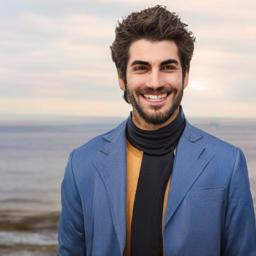
\includegraphics[width=0.24\linewidth]{figs/samples/adjmat1000_prompt_32_image_2.jpg}\,%
        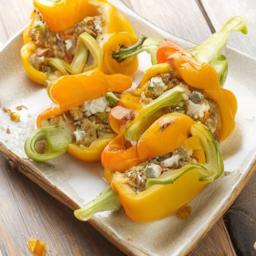
\includegraphics[width=0.24\linewidth]{figs/samples/adjmat1000_prompt_83_image_5.jpg}\,%
        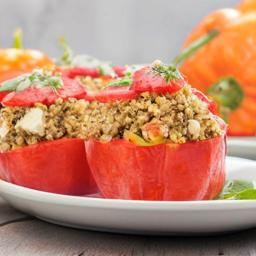
\includegraphics[width=0.24\linewidth]{figs/samples/adjmat1000_prompt_83_image_8.jpg}\\
        \rotatebox{90}{\;\; $\lambda=2500$}\,%
        
\includegraphics[width=0.24\linewidth]{figs/samples/adjmat2500_prompt_32_image_0.jpg}\,%
        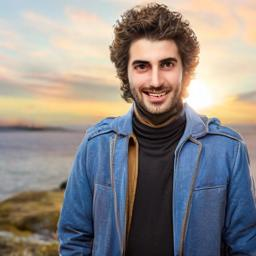
\includegraphics[width=0.24\linewidth]{figs/samples/adjmat2500_prompt_32_image_2.jpg}\,%
        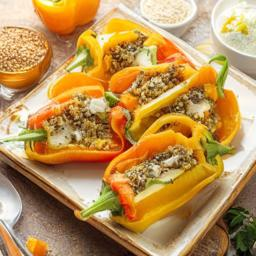
\includegraphics[width=0.24\linewidth]{figs/samples/adjmat2500_prompt_83_image_5.jpg}\,%
        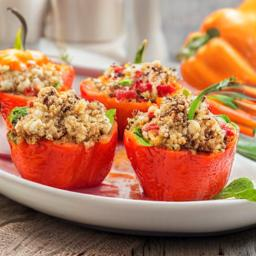
\includegraphics[width=0.24\linewidth]{figs/samples/adjmat2500_prompt_83_image_8.jpg}\\
        \rotatebox{90}{\; $\lambda=12500$}\,%
        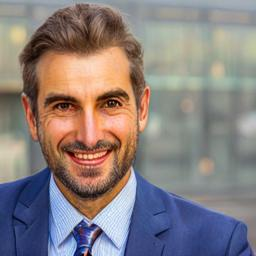
\includegraphics[width=0.24\linewidth]{figs/samples/adjmat12500_prompt_32_image_0.jpg}\,%
        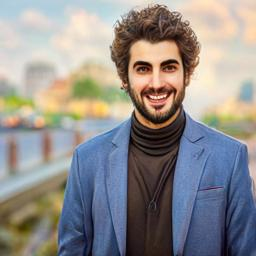
\includegraphics[width=0.24\linewidth]{figs/samples/adjmat12500_prompt_32_image_2.jpg}\,%
        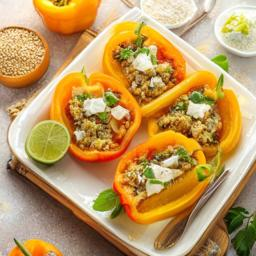
\includegraphics[width=0.24\linewidth]{figs/samples/adjmat12500_prompt_83_image_5.jpg}\,%
        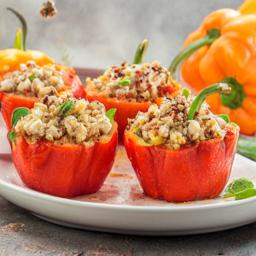
\includegraphics[width=0.24\linewidth]{figs/samples/adjmat12500_prompt_83_image_8.jpg}
        \caption*{Adjoint Matching (Ours)}
    \end{subfigure}\hfill
    \begin{subfigure}[t]{0.49\linewidth}
        \centering
        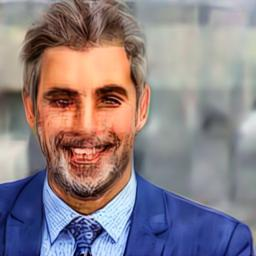
\includegraphics[width=0.24\linewidth]{figs/samples/draft1000_prompt_32_image_0.jpg}\,%
        
\includegraphics[width=0.24\linewidth]{figs/samples/draft1000_prompt_32_image_2.jpg}\,%
        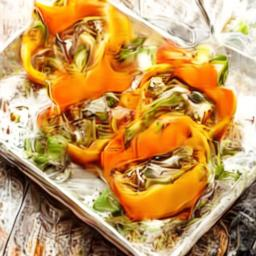
\includegraphics[width=0.24\linewidth]{figs/samples/draft1000_prompt_83_image_5.jpg}\,%
        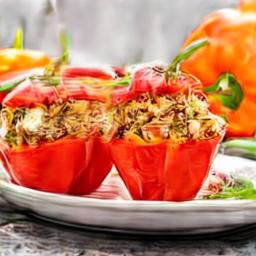
\includegraphics[width=0.24\linewidth]{figs/samples/draft1000_prompt_83_image_8.jpg}\,%
        \rotatebox[origin=r]{270}{$1000$ itrs. }\\
        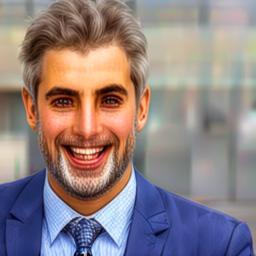
\includegraphics[width=0.24\linewidth]{figs/samples/draft2000_prompt_32_image_0.jpg}\,%
        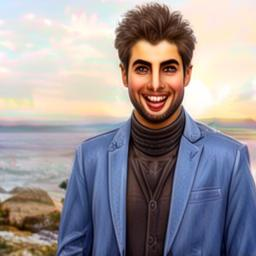
\includegraphics[width=0.24\linewidth]{figs/samples/draft2000_prompt_32_image_2.jpg}\,%
        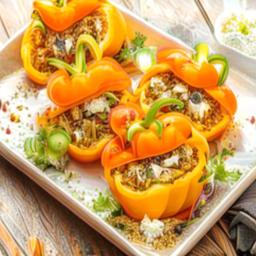
\includegraphics[width=0.24\linewidth]{figs/samples/draft2000_prompt_83_image_5.jpg}\,%
        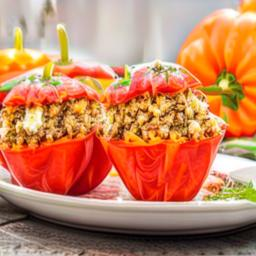
\includegraphics[width=0.24\linewidth]{figs/samples/draft2000_prompt_83_image_8.jpg}\,%
        \rotatebox[origin=r]{270}{$2000$ itrs. }\\
        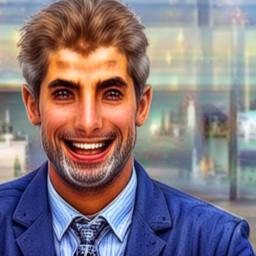
\includegraphics[width=0.24\linewidth]{figs/samples/draft4000_prompt_32_image_0.jpg}\,%
        \includegraphics[width=0.24\linewidth]{figs/samples/draft4000_prompt_32_image_2.jpg}\,%
        \includegraphics[width=0.24\linewidth]{figs/samples/draft4000_prompt_83_image_5.jpg}\,%
        \includegraphics[width=0.24\linewidth]{figs/samples/draft4000_prompt_83_image_8.jpg}\,%
        \rotatebox[origin=r]{270}{$4000$ itrs. }
        \caption*{DRaFT-1}
    \end{subfigure}
    \caption{Our proposed Adjoint Matching using the memoryless SOC formulation introduces a much more principled way of trading off how close to stay to the base model while optimizing the reward model. In contrast, baseline methods such as DRaFT-1 only optimize the reward model and must rely on early stopping to perform this trade off, resulting in a much more sensitive hyperparameter. Samples are produced using $\sigma(t)=0$ with the same noise sample. Text prompts: ``\textit{Handsome Smiling man in blue jacket portrait}'' and ``\textit{Quinoa and Feta Stuffed Baby Bell Peppers}''.}
    \label{fig:ablation_tradeoff_lambda}
\end{figure}

\begin{figure}[t!]
    \centering
    \begin{subfigure}[t]{0.49\linewidth}
        \centering
        \rotatebox{90}{\;\;\; $w=0.0$}\,%
        \includegraphics[width=0.24\linewidth]{figs/samples/adjmat0.0_prompt_37_image_3.jpg}\,%
        \includegraphics[width=0.24\linewidth]{figs/samples/adjmat0.0_prompt_37_image_5.jpg}\,%
        \includegraphics[width=0.24\linewidth]{figs/samples/adjmat0.0_prompt_37_image_6.jpg}\,%
        \includegraphics[width=0.24\linewidth]{figs/samples/adjmat0.0_prompt_37_image_7.jpg}\\
        \rotatebox{90}{\;\;\; $w=1.0$}\,%
        \includegraphics[width=0.24\linewidth]{figs/samples/adjmat1.0_prompt_37_image_3.jpg}\,%
        \includegraphics[width=0.24\linewidth]{figs/samples/adjmat1.0_prompt_37_image_5.jpg}\,%
        \includegraphics[width=0.24\linewidth]{figs/samples/adjmat1.0_prompt_37_image_6.jpg}\,%
        \includegraphics[width=0.24\linewidth]{figs/samples/adjmat1.0_prompt_37_image_7.jpg}\\
        \rotatebox{90}{\;\;\; $w=4.0$}\,%
        \includegraphics[width=0.24\linewidth]
        {figs/samples/adjmat4.0_prompt_37_image_3.jpg}\,%
        \includegraphics[width=0.24\linewidth]{figs/samples/adjmat4.0_prompt_37_image_5.jpg}\,%
        \includegraphics[width=0.24\linewidth]{figs/samples/adjmat4.0_prompt_37_image_6.jpg}\,%
        \includegraphics[width=0.24\linewidth]{figs/samples/adjmat4.0_prompt_37_image_7.jpg}
        \caption*{Text prompt: ``\textit{Man sitting on sofa at home in front of fireplace and using laptop computer, rear view}''}
    \end{subfigure}\hfill
    \begin{subfigure}[t]{0.49\linewidth}
        \centering
        \includegraphics[width=0.24\linewidth]{figs/samples/adjmat0.0_prompt_74_image_6.jpg}\,%
        \includegraphics[width=0.24\linewidth]{figs/samples/adjmat0.0_prompt_74_image_7.jpg}\,%
        \includegraphics[width=0.24\linewidth]{figs/samples/adjmat0.0_prompt_74_image_8.jpg}\,%
        \includegraphics[width=0.24\linewidth]{figs/samples/adjmat0.0_prompt_74_image_9.jpg}\\
        \includegraphics[width=0.24\linewidth]{figs/samples/adjmat1.0_prompt_74_image_6.jpg}\,%
        \includegraphics[width=0.24\linewidth]{figs/samples/adjmat1.0_prompt_74_image_7.jpg}\,%
        \includegraphics[width=0.24\linewidth]{figs/samples/adjmat1.0_prompt_74_image_8.jpg}\,%
        \includegraphics[width=0.24\linewidth]{figs/samples/adjmat1.0_prompt_74_image_9.jpg}\\
        \includegraphics[width=0.24\linewidth]{figs/samples/adjmat4.0_prompt_74_image_6.jpg}\,%
        \includegraphics[width=0.24\linewidth]{figs/samples/adjmat4.0_prompt_74_image_7.jpg}\,%
        \includegraphics[width=0.24\linewidth]{figs/samples/adjmat4.0_prompt_74_image_8.jpg}\,%
        \includegraphics[width=0.24\linewidth]{figs/samples/adjmat4.0_prompt_74_image_9.jpg}
        \caption*{Text prompt: ``\textit{3D World Food Day Morocco}''}
    \end{subfigure}
    \caption{
    Generated samples from varying classifier-free guidance weight $w$, from an Adjoint Matching fine-tuned model. 
    Higher guidance increases text-to-image consistency but loses diversity and has use cases for generating highly structured images such as 3D renderings.
    Corresponding samples from the base model can be found in \Cref{fig:ablation_tradeoff_cfg_base}. 
    }
    \label{fig:ablation_tradeoff_cfg}
\end{figure}

\begin{figure}
    \centering
    \includegraphics[width=0.65\linewidth]{figs/metrics_relationship_plots/legend.pdf}\\
    \includegraphics[width=0.325\linewidth]{figs/metrics_relationship_plots/dreamsim_diversity_vs_clipscore.pdf}
    \includegraphics[width=0.325\linewidth]{figs/metrics_relationship_plots/dreamsim_diversity_vs_hps_v2.pdf}
    \includegraphics[width=0.325\linewidth]{figs/metrics_relationship_plots/hps_v2_vs_clipscore.pdf}
    \caption{Tradeoffs between different aspects of generative models: text-to-image consistency (ClipScore), sample diversity for each prompt (DreamSim Diversity), and generalization to unseen human preferences (HPS v2). Different points are obtained from varying values of $\lambda$ for Adjoint Matching and varying number of fine-tuning iterations for the DRaFT-1 baseline. Overall, we find our proposed method Adjoint Matching has the best Pareto fronts.}
    \label{fig:tradeoffs}
\end{figure}

We experimentally validate our proposed method on reward fine-tuning a Flow Matching base model \citep{lipman2023flow}. In particular, we use the usual setup of pre-training an autoencoder for 512$\times$512 resolution images, then training a text-conditional Flow Matching model on the latent variables with a U-net architecture \citep{long2015fully}, similar to the setup in \citet{rombach2022high}. We pre-trained our base model using a dataset of licensed text and image pairs. Then for fine-tuning, we consider the reward function:
\begin{talign}
    r(x) := \lambda \times \texttt{RewardModel}(x)
\end{talign}
corresponding to a scaled version of the reward model, which we take to be ImageReward~\citep{xu2023imagereward}. Different values of $\lambda$ provide different tradeoffs between the KL regularization and the reward model \eqref{eq:kl_regularized_interpretation}.

For evaluation and benchmarking purposes, we report metrics that separately quantify text-to-image consistency, human preference, and sample diversity, capturing the tradeoff between each aspect of generative models~\citep{astolfi2024consistency}. For consistency, we make use of the standard ClipScore \citep{hessel2021clipscore} and PickScore \citep{kirstain2023pickapic}; for generalization to unseen human preferences, we use the HPSv2 model \citep{wu2023human}; and for diversity, we compute averages of pairwise distances of the DreamSim features \citep{fu2023learning}. More details are provided in \Cref{subsec:evaluation_metrics}.
% \ricky{TODO appendix}.

As our baselines, we consider the DPO \citep{wallace2023diffusion}, ReFL \citep{xu2023imagereward}, and DRaFT-K algorithms \citep{clark2024directly}. DPO does not use gradients from the reward function, while ReFL and DRaFT make use of heuristic gradient stopping approaches to stay close to the base generative model. 
Out of these baseline methods, we find that DRaFT-1 performs the best, so we perform additional ablation experiments comparing to this method.
Within the same SOC formulation as our method, we also consider the discrete and continuous adjoint methods. We provide full experimental details in \Cref{sec:experimental_details}; an important implementation detail is that we slightly offset $\sigma(t)$ in order to avoid division by zero.

\paragraph{Evaluation results.} In \Cref{tab:evaluation_metrics} we report the evaluation metrics for the baselines as well as our proposed Adjoint Matching approach. We compare each method at roughly the same wall clock time (see the times and number of iterations in \Cref{table:metrics_multiprompt_alternative}, and comments in \Cref{subsec:remarks_computational_cost}).
We find that across all metrics, our proposed memoryless SOC formulation outperforms existing baseline methods. The choice of SOC algorithms also obviously favors Adjoint Matching over continuous and discrete adjoint methods, which result in poorer consistency and human preference metrics.

\paragraph{Ablation: base model vs. reward tradeoff.} We note that the scaling in front of the reward model $\lambda$ determines how strongly the we should prefer the reward model over the base model. As such, we see a natural tradeoff curve: higher $\lambda$ results in better consistency and human preference, but lower diversity in the generated samples. Overall, we find that Adjoint Matching performs stably across all values of $\lambda$. Our method of regularizing the fine-tuning procedure through memoryless SOC works much better than baseline methods which often must employ early stopping. We show the qualitative effect of varying $\lambda$ in \Cref{fig:ablation_tradeoff_lambda}, while for the DRaFT-1 baseline we show the effect of varying the number of fine-tuning iterations.

\paragraph{Ablation: classifier-free guidance.} We note that it is possible to apply classifier-free guidance (CFG; \citet{ho2022classifier,zheng2023guided}) after fine-tuning. We use the formula $(1+w) v(x, t | y) - w v(x, t)$, where $w$ is the guidance weight, $v(x, t | y)$ is a fine-tuned text-to-image model while $v(x, t)$ is an unconditional image model.
This is not principled as only the conditional model is fine-tuned, but generally it is unclear what distribution guided models sample from anyhow. 
In \Cref{fig:tradeoffs} we show the evaluation metrics with classifier-free guidance applied. Comparing three different guidance weight values, we see a higher weight does improve text-to-image consistency, and to some extent, human preference, but this comes at the cost of being worse in terms of diversity. We show qualitative differences in \Cref{fig:ablation_tradeoff_cfg}.

\section{Conclusion}
\label{sec:conclusion}

We investigate the problem of fine-tuning dynamical generative models such as Flow Matching and propose the use of a stochastic optimal control (SOC) formulation with a memoryless noise schedule. 
This ensures we converge to the same tilted distribution that the large language modeling literature uses for learning from human feedback. 
In particular, the memoryless noise schedule corresponds to DDPM sampling for diffusion models and a new Memoryless Flow Matching generative process for flow models. 
In conjunction, we propose a novel training algorithm for solving stochastic optimal control problems, by casting SOC as a regression problem, which we call the Adjoint Matching objective. 
Empirically, we find that our memoryless SOC formulation works better than multiple existing works on fine-tuning diffusion models, and our Adjoint Matching algorithm outperforms related gradient-based methods.
In summary, we are the first to provide a theoretically-driven algorithm for fine-tuning Flow Matching models, and we find that our approach significantly outperforms baseline methods across multiple axes of evaluation---text-to-image consistency, generalization to unseen human preference, and sample diversity---on large-scale text-to-image generation.

\bibliographystyle{assets/plainnat}
\bibliography{biblio}

\clearpage
\newpage
\beginappendix

\tableofcontents

\starttocentries

\clearpage
\newpage

\section{Additional Figures \& Tables}
\label{sec:additional_figures_tables}

\begin{figure}[h!]
    \centering
    \includegraphics[width=0.46\linewidth]{figs/training_plots/reward_plot.png}
    \includegraphics[width=0.46\linewidth]{figs/training_plots/control_term_plot.png}
    \includegraphics[width=0.46\linewidth]{figs/training_plots/clipscore_plot.png}
    \caption{Average values of ImageReward (reward function), control cost ($\int_0^t \frac{1}{2} \|u(X^u_t,t)\|^2 \, \mathrm{d}t$), and ClipScore vs. wall-clock time for Adjoint Matching and our baselines. Lines show averages over three fine-tuning runs, evaluating on separate test datasets of size 200. Confidence intervals show standard errors of estimates.}
    \label{fig:training_figures}
\end{figure}

\begin{table}[h!]
\centering
{\small
\begin{tabular}{lcccccc}
    \toprule
    Fine-tuning & Fine-tuning & Sampling & \multirow{2}{*}{ImageReward$\, \uparrow$} & ClipScore & PickScore & Total time (s) /
    \\
    loss & $\sigma(t)$ & $\sigma(t)$ &  & diversity$\, \uparrow$ & diversity$\, \uparrow$ & \# iterations \\
    \midrule
    None & \multirow{2}{*}{N/A} & $\sqrt{2 \eta_t}$ & $-$1.384{\tiny$\pm$0.040} & 28.07{\tiny$\pm$1.40} & 1.63{\tiny$\pm$0.08} & \multirow{2}{*}{N/A} 
    \\
    ($\mathrm{CFG}=1.0$)                    &                     & 0                 & $-$0.920{\tiny$\pm$0.042} & 30.29{\tiny$\pm$1.53} & 1.82{\tiny$\pm$0.09} \\
    \midrule
    \multirow{2}{*}{DRaFT-1}           & $\sqrt{2 \eta_t}$ & $\sqrt{2 \eta_t}$ & 1.357{\tiny$\pm$0.039} & 16.86{\tiny$\pm$0.98} & 1.21{\tiny$\pm$0.07} 
    & 140k{\tiny$\pm$5.9k}
    \\
                                       & 0                 & 0                 & 1.251{\tiny$\pm$0.040} & 16.76{\tiny$\pm$1.06} & 1.27{\tiny$\pm$0.07} 
    & / 4000 
    \\
    \addlinespace
    \multirow{2}{*}{DRaFT-40}          & $\sqrt{2 \eta_t}$ & $\sqrt{2 \eta_t}$ & $-$0.560{\tiny$\pm$0.138} & 24.07{\tiny$\pm$1.37} & 1.64{\tiny$\pm$0.12} 
    & 148k{\tiny$\pm$4.2k} 
    \\
                                       & 0                 & 0                 & 0.424{\tiny$\pm$0.042} & 20.99{\tiny$\pm$1.54} & 1.67{\tiny$\pm$0.08} 
    & / 1500 
    \\
    \addlinespace
    \multirow{2}{*}{DPO}          & $\sqrt{2 \eta_t}$ & $\sqrt{2 \eta_t}$ & $-$1.386{\tiny$\pm$0.033} & 27.80{\tiny$\pm$1.40} & 1.62{\tiny$\pm$0.08} 
    & 118k{\tiny$\pm$0.6k} 
    \\
                                       & 0                 & 0                 & $-$0.957{\tiny$\pm$0.040} & 29.81{\tiny$\pm$1.43} & 1.68{\tiny$\pm$0.10} 
    & / 1000
    \\
    \addlinespace
    \multirow{2}{*}{ReFL}              & $\sqrt{2 \eta_t}$ & $\sqrt{2 \eta_t}$ & 0.687{\tiny$\pm$0.085} & 19.49{\tiny$\pm$1.76} & 1.22{\tiny$\pm$0.08} 
    & 173k{\tiny$\pm$10.9k}
    \\
                                       & 0                 & 0                 & 0.709{\tiny$\pm$0.080} & 18.39{\tiny$\pm$1.11} & 1.31{\tiny$\pm$0.10} 
    & / 6000 
    \\
    \midrule % \addlinespace
    Cont. Adjoint & \multirow{2}{*}{$\sqrt{2 \eta_t}$} & $\sqrt{2 \eta_t}$ & $-$0.448{\tiny$\pm$0.135} & 26.97{\tiny$\pm$1.37} & 1.82{\tiny$\pm$0.09} 
    & 153k{\tiny$\pm$0.9k}
    \\
    $\lambda = 12500$                     &                                    & 0                 & $-$0.249{\tiny$\pm$0.116} & 26.25{\tiny$\pm$1.30} & 1.90{\tiny$\pm$0.10} 
    & / 750  
    \\
    \addlinespace
    Disc. Adjoint & \multirow{2}{*}{$\sqrt{2 \eta_t}$} & $\sqrt{2 \eta_t}$ & $-$0.557{\tiny$\pm$0.113} & 30.40{\tiny$\pm$2.39} & 1.91{\tiny$\pm$0.09} 
    & 152k{\tiny$\pm$1.5k}
    \\
    $\lambda = 12500$                    &                                    & 0                 & $-$0.552{\tiny$\pm$0.041} & 28.37{\tiny$\pm$2.26} & 1.97{\tiny$\pm$0.09} 
    & / 1000 
    \\
    \midrule % \addlinespace
    Adj.-Matching  & \multirow{2}{*}{$\sqrt{2 \eta_t}$} & $\sqrt{2 \eta_t}$ & 0.550{\tiny$\pm$0.043} & 23.00{\tiny$\pm$1.27} & 1.65{\tiny$\pm$0.08} 
    &  
    \\
    $\lambda = 1000$                     &                                    & 0                 & 0.454{\tiny$\pm$0.055} & 22.76{\tiny$\pm$1.40} & 1.73{\tiny$\pm$0.09} 
    % &  
    \\
    \addlinespace
    Adj.-Matching & \multirow{2}{*}{$\sqrt{2 \eta_t}$} & $\sqrt{2 \eta_t}$ & 0.755{\tiny$\pm$0.040} & 21.33{\tiny$\pm$1.71} & 1.55{\tiny$\pm$0.08} 
    & 156k{\tiny$\pm$1.9k}
    \\
    $\lambda = 2500$                     &                                    & 0                 & 0.671{\tiny$\pm$0.047} & 21.42{\tiny$\pm$1.54} & 1.64{\tiny$\pm$0.08}
    & / 1000 
    \\
    \addlinespace
    Adj.-Matching  & \multirow{2}{*}{$\sqrt{2 \eta_t}$} & $\sqrt{2 \eta_t}$ & 0.882{\tiny$\pm$0.058} & 20.49{\tiny$\pm$1.48} & 1.50{\tiny$\pm$0.09} 
    & 
    \\
    $\lambda = 12500$                    &                                    & 0                 & 0.778{\tiny$\pm$0.050} & 20.34{\tiny$\pm$1.49} & 1.57{\tiny$\pm$0.09}
    &  
    \\
    \bottomrule
\end{tabular}
}
\caption{Metrics for various fine-tuning methods for text-to-image generation. The second and third columns show the noise schedules $\sigma(t)$ used for fine-tuning and for inference: $\sigma(t) = \sqrt{2\eta_t}$ corresponds to Memoryless Flow Matching, %\eqref{eq:memoryless_FM_sde}, 
and $\sigma(t) = 0$ to the Flow Matching ODE \eqref{eq:FM_ode}. Confidence intervals show standard errors of estimates; computed over 3 runs of the fine-tuning algorithm on separate fine-tuning prompt datasets of size 40000 each. Test prompt sets are of size 1000, and also different for each run.}
\label{table:metrics_multiprompt_diversity}
\end{table}

\begin{table}[h!]
\centering
{\footnotesize
\begin{tabular}{lcccccccc}
    \toprule
    Fine-tun. & Fine-tun. & Generat. & \multirow{2}{*}{ImageReward$\, \uparrow$} & \multirow{2}{*}{ClipScore$\, \uparrow$} & \multirow{2}{*}{PickScore$\, \uparrow$} & \multirow{2}{*}{HPS v2$\, \uparrow$} & DreamSim & Runtime/ \\
    loss & $\sigma(t)$ & $\sigma(t)$ &  & &  &  & diversity$\, \uparrow$ & $\#$iter. \\
    % \midrule
    % \multirow{2}{*}{None (Base)} & \multirow{2}{*}{N/A} & $\sqrt{2 \eta_t}$ & $-\! \pm \!-$ & $-\! \pm \!-$ & $-\! \pm \!-$ & $-\! \pm \!-$ & \multirow{2}{*}{N/A} \\
    %                              &                     & 0                 & $-\! \pm \!-$ & $-\! \pm \!-$ & $-\! \pm \!-$ & $-\! \pm \!-$ &  \\
    \midrule % \addlinespace
    \multirow{2}{*}{ReFL}              & $\sqrt{2 \eta_t}$ & $\sqrt{2 \eta_t}$ & 0.459{\tiny$\pm$0.096} & 28.46{\tiny$\pm$0.25} & 18.77{\tiny$\pm$0.09} & 22.54{\tiny$\pm$0.17} & 37.51{\tiny$\pm$3.50} & 43k{\tiny$\pm$2.7k} \\
                                       & 0                 & 0                 & 0.330{\tiny$\pm$0.114} & 29.63{\tiny$\pm$0.61} & 19.08{\tiny$\pm$0.18} & 22.46{\tiny$\pm$0.77} & 39.51{\tiny$\pm$1.30} & / 1500 \\
    \addlinespace
    \multirow{2}{*}{DRaFT-1}           & $\sqrt{2 \eta_t}$ & $\sqrt{2 \eta_t}$ & 0.913{\tiny$\pm$0.068} & 29.80{\tiny$\pm$0.22} & 19.16{\tiny$\pm$0.06} & 23.63{\tiny$\pm$0.16} & 35.21{\tiny$\pm$1.93} & 35k{\tiny$\pm$1.5k} \\
                                       & 0                 & 0                 & 0.626{\tiny$\pm$0.195} & 30.48{\tiny$\pm$0.32} & 18.91{\tiny$\pm$0.34} & 21.92{\tiny$\pm$1.63} & 38.52{\tiny$\pm$2.01} & / 1000 \\
    \addlinespace
    \multirow{2}{*}{Draft-40}          & $\sqrt{2 \eta_t}$ & $\sqrt{2 \eta_t}$ & $-$1.427{\tiny$\pm$0.267} & 23.39{\tiny$\pm$1.72} & 17.24{\tiny$\pm$0.45} & 15.72{\tiny$\pm$1.80} & 41.98{\tiny$\pm$2.14} & 49k{\tiny$\pm$1.4k} \\
                                       & 0                 & 0                 & $-$0.097{\tiny$\pm$0.052} & 29.12{\tiny$\pm$0.41} & 18.97{\tiny$\pm$0.14} & 21.93{\tiny$\pm$0.20} & 46.35{\tiny$\pm$1.34} & / 500 \\
    \midrule % \addlinespace
    Adj.-Match.  & \multirow{2}{*}{$\sqrt{2 \eta_t}$} & $\sqrt{2 \eta_t}$ & 0.107{\tiny$\pm$0.046} & 29.37{\tiny$\pm$0.25} & 19.05{\tiny$\pm$0.07} & 22.79{\tiny$\pm$0.20} & 46.38{\tiny$\pm$1.36} &  \\
    $\lambda = 1000$                     &                                    & 0                 & 0.051{\tiny$\pm$0.044} & 30.58{\tiny$\pm$0.17} & 19.31{\tiny$\pm$0.07} & 21.93{\tiny$\pm$0.23} & 48.12{\tiny$\pm$1.56} &  \\
    \addlinespace
    Adj.-Match. & \multirow{2}{*}{$\sqrt{2 \eta_t}$} & $\sqrt{2 \eta_t}$ & 0.199{\tiny$\pm$0.068} & 29.27{\tiny$\pm$0.21} & 19.07{\tiny$\pm$0.10} & 22.98{\tiny$\pm$0.30} & 45.03{\tiny$\pm$1.61} & 39k{\tiny$\pm$0.5k} \\
    $\lambda = 2500$                     &                                    & 0                 & 0.106{\tiny$\pm$0.067} & 30.43{\tiny$\pm$0.24} & 19.32{\tiny$\pm$0.11} & 22.16{\tiny$\pm$0.33} & 47.61{\tiny$\pm$1.49} & / 250 \\
    \addlinespace
    Adj.-Match.  & \multirow{2}{*}{$\sqrt{2 \eta_t}$} & $\sqrt{2 \eta_t}$ & 0.299{\tiny$\pm$0.095} & 29.61{\tiny$\pm$0.37} & 19.26{\tiny$\pm$0.14} & 23.67{\tiny$\pm$0.27} & 43.36{\tiny$\pm$1.93} &  \\
    $\lambda = 12500$                    &                                    & 0                 & 0.224{\tiny$\pm$0.051} & 30.70{\tiny$\pm$0.23} & 19.52{\tiny$\pm$0.11} & 22.93{\tiny$\pm$0.21} & 44.62{\tiny$\pm$1.79} &  \\
    \midrule % \addlinespace
    Cont. Adj. & \multirow{2}{*}{$\sqrt{2 \eta_t}$} & $\sqrt{2 \eta_t}$ & $-$0.910{\tiny$\pm$0.116} & 26.29{\tiny$\pm$0.44} & 18.06{\tiny$\pm$0.16} & 18.86{\tiny$\pm$0.88} & 51.60{\tiny$\pm$1.97} & 51k{\tiny$\pm$0.3k} \\
    $\lambda = 12500$                     &                                    & 0                 & $-$0.681{\tiny$\pm$0.051} & 28.50{\tiny$\pm$0.19} & 18.69{\tiny$\pm$0.11} & 19.90{\tiny$\pm$0.50} & 50.87{\tiny$\pm$1.52} & / 250 \\
    \addlinespace
    Disc. Adj. & \multirow{2}{*}{$\sqrt{2 \eta_t}$} & $\sqrt{2 \eta_t}$ & $-$0.978{\tiny$\pm$0.123} & 26.68{\tiny$\pm$0.76} & 18.51{\tiny$\pm$0.11} & 18.53{\tiny$\pm$0.28} & 55.95{\tiny$\pm$1.70} & 38k{\tiny$\pm$0.4k} \\
    $\lambda = 12500$                    &                                    & 0                 & $-$0.791{\tiny$\pm$0.065} & 28.66{\tiny$\pm$0.33} & 18.51{\tiny$\pm$0.11} & 18.53{\tiny$\pm$0.28} & 54.78{\tiny$\pm$2.00} & / 250 \\
    \bottomrule
\end{tabular}
}
\caption{Additional metrics for various fine-tuning methods for text-to-image generation, which complement the ones in \Cref{tab:evaluation_metrics} (both tables correspond to the same runs). The second and third columns show the noise schedules $\sigma(t)$ used for fine-tuning and for inference: $\sigma(t) = \sqrt{2\eta_t}$ corresponds to Memoryless Flow Matching, 
% \eqref{eq:memoryless_FM_sde}, 
and $\sigma(t) = 0$ to the Flow Matching ODE \eqref{eq:FM_ode}.
}
\label{table:metrics_multiprompt_alternative}
\end{table}

\begin{table}[h!]
\centering
{\footnotesize
\begin{tabular}{lllccccccc}
    \toprule
    \multirow{2}{*}{$w$} & Fine-tuning & $\#$iter. & Fine-tun. & Sampl.  & \multirow{2}{*}{ImageReward$\, \uparrow$} & \multirow{2}{*}{ClipScore$\, \uparrow$} & \multirow{2}{*}{PickScore$\, \uparrow$} & \multirow{2}{*}{HPS v2$\, \uparrow$} & DreamSim \\
     & loss & / $\lambda$ & $\sigma(t)$ & $\sigma(t)$ &  &  &  &  & diversity$\, \uparrow$ \\
    \midrule
    \multirow{2}{*}{0.0} & \multirow{2}{*}{None} &  \multirow{2}{*}{N/A}        & \multirow{2}{*}{N/A}          & $\sqrt{2 \eta_t}$         & $-$1.384{\tiny$\pm$0.040} & 24.15{\tiny$\pm$0.26} & 17.25{\tiny$\pm$0.06} & 16.19{\tiny$\pm$0.17} & 53.60{\tiny$\pm$1.37} \\
     &  &       &                & 0                 & $-$0.920{\tiny$\pm$0.042} & 28.32{\tiny$\pm$0.22} & 18.15{\tiny$\pm$0.07} & 17.89{\tiny$\pm$0.16} & \textbf{56.53{\tiny$\pm$1.52}}       
                                    \\
    \midrule
    \multirow{7}{*}{0.0} & \multirow{7}{*}{DRaFT-1} &  \multirow{2}{*}{1000}       & $\sqrt{2 \eta_t}$ & $\sqrt{2 \eta_t}$ & 0.913{\tiny$\pm$0.068} & 29.80{\tiny$\pm$0.22} & 19.16{\tiny$\pm$0.06} & 23.63{\tiny$\pm$0.16} & 35.21{\tiny$\pm$1.93} \\
    & &  & 0                 & 0                 & 0.626{\tiny$\pm$0.195} & 30.48{\tiny$\pm$0.32} & 18.91{\tiny$\pm$0.34} & 21.92{\tiny$\pm$1.63} & 38.52{\tiny$\pm$2.01} \\
    % \midrule
    \addlinespace
     &  &  \multirow{2}{*}{2000}       & $\sqrt{2 \eta_t}$ & $\sqrt{2 \eta_t}$ & 1.204{\tiny$\pm$0.046} & 29.90{\tiny$\pm$0.43} & 19.29{\tiny$\pm$0.12} & 24.40{\tiny$\pm$0.27} & 28.51{\tiny$\pm$1.68} \\
                                   & &  & 0                 & 0                 & 1.052{\tiny$\pm$0.088} & 30.65{\tiny$\pm$0.24} & 19.27{\tiny$\pm$0.11} & 23.81{\tiny$\pm$0.44} & 32.11{\tiny$\pm$2.37} \\
    % \midrule
    \addlinespace
    & &  \multirow{2}{*}{3000}       & $\sqrt{2 \eta_t}$ & $\sqrt{2 \eta_t}$ & \textbf{1.307{\tiny$\pm$0.041}} & 29.96{\tiny$\pm$0.22} & 19.31{\tiny$\pm$0.06} & 24.42{\tiny$\pm$0.13} & 26.57{\tiny$\pm$1.32} \\
                                   & &  & 0                 & 0                 & 1.173{\tiny$\pm$0.058} & 30.86{\tiny$\pm$0.25} & 19.37{\tiny$\pm$0.06} & 24.17{\tiny$\pm$0.23} & 29.69{\tiny$\pm$1.30}
    \\
    \addlinespace
    & &  \multirow{2}{*}{4000}       & $\sqrt{2 \eta_t}$ & $\sqrt{2 \eta_t}$ & \textbf{1.357{\tiny$\pm$0.039}} & 30.18{\tiny$\pm$0.24} & 19.38{\tiny$\pm$0.08} & 24.61{\tiny$\pm$0.17} & 25.54{\tiny$\pm$0.99} \\
                                   & &  & 0                 & 0                 & 1.251{\tiny$\pm$0.040} & 30.95{\tiny$\pm$0.28} & 19.37{\tiny$\pm$0.06} & 24.37{\tiny$\pm$0.17} & 27.39{\tiny$\pm$1.14}
    \\
    \midrule
    \multirow{7}{*}{0.0} & \multirow{7}{*}{Adj.-Match.} & \multirow{2}{*}{1000} & $\sqrt{2 \eta_t}$ & $\sqrt{2 \eta_t}$  & 0.550{\tiny$\pm$0.043} & 30.36{\tiny$\pm$0.22} & 19.29{\tiny$\pm$0.08} & 24.12{\tiny$\pm$0.17} & 40.89{\tiny$\pm$1.50} \\
     & &  & 0                 & 0                 & 0.454{\tiny$\pm$0.055} &  31.41{\tiny$\pm$0.22} & 19.57{\tiny$\pm$0.09} & 23.29{\tiny$\pm$0.18} & 43.10{\tiny$\pm$1.76} \\
    \addlinespace
    & & \multirow{2}{*}{2500} & $\sqrt{2 \eta_t}$ & $\sqrt{2 \eta_t}$ & 0.755{\tiny$\pm$0.040} & 30.59{\tiny$\pm$0.40} & 19.49{\tiny$\pm$0.10} & 24.85{\tiny$\pm$0.23} & 37.07{\tiny$\pm$1.47} \\
    & &  & 0 & 0 & 0.671{\tiny$\pm$0.047} & 31.64{\tiny$\pm$0.21} & 19.71{\tiny$\pm$0.09} & 24.12{\tiny$\pm$0.27} & 39.88{\tiny$\pm$1.59} \\
    \addlinespace
    & & \multirow{2}{*}{12500} & $\sqrt{2 \eta_t}$ & $\sqrt{2 \eta_t}$ & 0.882{\tiny$\pm$0.058} & 30.62{\tiny$\pm$0.30} & 19.50{\tiny$\pm$0.09} & 24.95{\tiny$\pm$0.28} & 34.50{\tiny$\pm$1.33} \\
    & &  & 0 & 0 & 0.778{\tiny$\pm$0.050} & 31.65{\tiny$\pm$0.19} & 19.76{\tiny$\pm$0.08} & 24.49{\tiny$\pm$0.27} & 37.24{\tiny$\pm$1.57} \\
    \midrule
    \multirow{2}{*}{1.0} & \multirow{2}{*}{None} &  \multirow{2}{*}{N/A}        & \multirow{2}{*}{N/A}          & $\sqrt{2 \eta_t}$         & $-$0.269{\tiny$\pm$0.050} & 30.41{\tiny$\pm$0.22} & 18.74{\tiny$\pm$0.07} & 20.47{\tiny$\pm$0.18} & 43.82{\tiny$\pm$1.24} \\
     &  &       &                & 0                 & $-$0.123{\tiny$\pm$0.041} & 31.83{\tiny$\pm$0.17} & 19.28{\tiny$\pm$0.07} & 20.95{\tiny$\pm$0.16} & 42.59{\tiny$\pm$1.23}                             
                                    \\
    \midrule
    \multirow{6}{*}{1.0} & \multirow{6}{*}{DRaFT-1} &  \multirow{2}{*}{1000}        & $\sqrt{2 \eta_t}$          & $\sqrt{2 \eta_t}$         & 1.123{\tiny$\pm$0.051} & 32.06{\tiny$\pm$0.19} & 19.69{\tiny$\pm$0.06} & 24.56{\tiny$\pm$0.17} & 28.25{\tiny$\pm$1.55} \\
     &  &       & 0                 & 0                 & 0.856{\tiny$\pm$0.167} & 32.32{\tiny$\pm$0.25} & 19.38{\tiny$\pm$0.34} & 22.88{\tiny$\pm$1.54} & 29.98{\tiny$\pm$1.86} \\
    % \midrule
    \addlinespace
     &  &  2000        & 0                 & 0                 & 1.177{\tiny$\pm$0.053} & 32.36{\tiny$\pm$0.18} & 19.67{\tiny$\pm$0.08} & 24.48{\tiny$\pm$0.28} & 25.09{\tiny$\pm$1.82} \\
    % \midrule
    \addlinespace
    & & 3000 & 0                 & 0                 & 1.255{\tiny$\pm$0.038} & 32.36{\tiny$\pm$0.19} & 19.70{\tiny$\pm$0.06} & 24.64{\tiny$\pm$0.17} & 23.24{\tiny$\pm$1.19} \\
    \addlinespace
    & &  4000  & 0 & 0 & \textbf{1.296{\tiny$\pm$0.033}} & 32.30{\tiny$\pm$0.19} & 19.68{\tiny$\pm$0.06} & 24.71{\tiny$\pm$0.14} & 21.54{\tiny$\pm$0.96} \\
    \midrule
    \multirow{5}{*}{1.0} & \multirow{5}{*}{Adj.-Match.} & 1000 & 0                 & 0                 & 0.782{\tiny$\pm$0.044} & 33.05{\tiny$\pm$0.22} & 20.20{\tiny$\pm$0.09} & 24.81{\tiny$\pm$0.18} & 32.67{\tiny$\pm$1.26} \\
    \addlinespace
    & & \multirow{2}{*}{2500} & $\sqrt{2 \eta_t}$ & $\sqrt{2 \eta_t}$ & 1.027{\tiny$\pm$0.038} & 32.85{\tiny$\pm$0.21} & 20.08{\tiny$\pm$0.08} & \textbf{25.88{\tiny$\pm$0.20}} & 29.83{\tiny$\pm$1.00} \\
    & &  & 0 & 0 & 0.910{\tiny$\pm$0.040} & 33.20{\tiny$\pm$0.17} & 20.29{\tiny$\pm$0.09} & 25.39{\tiny$\pm$0.24} & 30.34{\tiny$\pm$1.51} \\
    \addlinespace
    & & 12500 & 0 & 0 & 0.985{\tiny$\pm$0.041} & 33.10{\tiny$\pm$0.18} & 20.28{\tiny$\pm$0.08} & \textbf{25.61{\tiny$\pm$0.27}} & 28.86{\tiny$\pm$1.37} \\
    \midrule
    \multirow{2}{*}{4.0} & \multirow{2}{*}{None} &  \multirow{2}{*}{N/A}        & \multirow{2}{*}{N/A}          & $\sqrt{2 \eta_t}$         & 0.277{\tiny$\pm$0.043} & 32.68{\tiny$\pm$0.18} & 19.50{\tiny$\pm$0.07} & 22.29{\tiny$\pm$0.16} & 35.12{\tiny$\pm$0.92} \\
     &  &       &                & 0                 & 0.209{\tiny$\pm$0.046} & 32.83{\tiny$\pm$0.17} & 19.79{\tiny$\pm$0.07} & 22.30{\tiny$\pm$0.17} & 32.05{\tiny$\pm$1.05}    
                                    \\
    \midrule
    \multirow{6}{*}{4.0} & \multirow{6}{*}{DRaFT-1} &  \multirow{2}{*}{1000}        & $\sqrt{2 \eta_t}$          & $\sqrt{2 \eta_t}$         & 1.062{\tiny$\pm$0.045} & 32.29{\tiny$\pm$0.16} & 19.48{\tiny$\pm$0.06} & 23.67{\tiny$\pm$0.13} & 25.03{\tiny$\pm$1.32} \\
     &  &       & 0                 & 0                 & 0.604{\tiny$\pm$0.395} & 31.80{\tiny$\pm$0.86} & 19.09{\tiny$\pm$0.53} & 21.69{\tiny$\pm$2.10} & 25.92{\tiny$\pm$2.57} \\
    % \midrule
    \addlinespace
     &  &  2000        & 0                 & 0                 & 1.112{\tiny$\pm$0.046} & 32.29{\tiny$\pm$0.20} & 19.34{\tiny$\pm$0.11} & 23.31{\tiny$\pm$0.22} & 21.02{\tiny$\pm$1.67} \\
    % \midrule
    \addlinespace
    & & 3000 & 0                 & 0                 & 1.151{\tiny$\pm$0.036} & 32.31{\tiny$\pm$0.21} & 19.36{\tiny$\pm$0.06} & 23.29{\tiny$\pm$0.14} & 19.53{\tiny$\pm$1.24} \\
    \addlinespace
    & &  4000  & 0 & 0 & 1.172{\tiny$\pm$0.040} & 32.20{\tiny$\pm$0.22} & 19.30{\tiny$\pm$0.07} & 23.20{\tiny$\pm$0.15} & 18.45{\tiny$\pm$1.06} \\
    \midrule
    \multirow{5}{*}{4.0} & \multirow{5}{*}{Adj.-Match.} & 1000 & 0                 & 0                 & 0.852{\tiny$\pm$0.046} & \textbf{33.50{\tiny$\pm$0.22}} & 20.31{\tiny$\pm$0.08} & 24.97{\tiny$\pm$0.19} & 25.83{\tiny$\pm$0.82} \\
    \addlinespace
    & & \multirow{2}{*}{2500} & $\sqrt{2 \eta_t}$ & $\sqrt{2 \eta_t}$ & 1.052{\tiny$\pm$0.039} & \textbf{33.51}{\tiny$\pm$0.19} & 20.15{\tiny$\pm$0.07} & \textbf{25.56{\tiny$\pm$0.18}} & 26.21{\tiny$\pm$0.73} \\
    & &  & 0 & 0 & 0.942{\tiny$\pm$0.042} & \textbf{33.61}{\tiny$\pm$0.19} & \textbf{20.35}{\tiny$\pm$0.08} & 25.34{\tiny$\pm$0.21} & 24.30{\tiny$\pm$0.86} \\
    \addlinespace
    & & 12500 & 0 & 0 & 1.007{\tiny$\pm$0.052} & \textbf{33.48{\tiny$\pm$0.20}} & 20.29{\tiny$\pm$0.08} & \textbf{25.50{\tiny$\pm$0.29}} & 23.48{\tiny$\pm$0.81} \\
    \bottomrule
\end{tabular}
}
\caption{ 
Evaluation metrics when using classifier-free guidance (CFG; \citet{ho2022classifier}).
}
\end{table}

\begin{table}[h!]
\centering
{\footnotesize
\begin{tabular}{llccccccc}
    \toprule
    LR / & Fine-tuning & Fine-tun. & Generat. & \multirow{2}{*}{ImageReward$\, \uparrow$} & \multirow{2}{*}{ClipScore$\, \uparrow$} & \multirow{2}{*}{PickScore$\, \uparrow$} & \multirow{2}{*}{HPS v2$\, \uparrow$} & DreamSim \\
    Adam $\beta_1$ & loss & $\sigma(t)$ & $\sigma(t)$ & & &  &  & diversity$\, \uparrow$ \\
    \midrule
    \num{3e-5} & DRaFT-1          & $\sqrt{2 \eta_t}$ & $\sqrt{2 \eta_t}$ & 1.467{\tiny$\pm$0.029} & 30.28{\tiny$\pm$0.56} & 19.37{\tiny$\pm$0.09} & 24.70{\tiny$\pm$0.15} & 21.20{\tiny$\pm$0.93} \\
               % &  &  & $\num{3e-5} / 0.97$ & $- \pm -$ & $- \pm -$ & $- \pm -$ & $- \pm -$ \\
    \addlinespace
    / \num{0.97} & Adj.-Match.  & \multirow{2}{*}{$\sqrt{2 \eta_t}$} & \multirow{2}{*}{$\sqrt{2 \eta_t}$} & \multirow{2}{*}{1.130{\tiny$\pm$0.034}} & \multirow{2}{*}{31.01{\tiny$\pm$0.27}} & \multirow{2}{*}{19.60{\tiny$\pm$0.08}} & \multirow{2}{*}{25.01{\tiny$\pm$0.25}} & \multirow{2}{*}{26.73{\tiny$\pm$0.88}} \\
    & $\lambda = 12500$                     &                                    &                 &  &  &  &  &  \\
    \midrule
    \num{2e-5} & Disc. Adj.  & $\sqrt{2 \eta_t}$ & $\sqrt{2 \eta_t}$ & $-$1.186{\tiny$\pm$0.553} & 21.95{\tiny$\pm$4.29} & 16.94{\tiny$\pm$0.95} & 12.34{\tiny$\pm$4.40} & 28.33{\tiny$\pm$10.26} \\
     / \num{0.95} & $\lambda = 12500$                     &  0                                  &  0               & $-$0.961{\tiny$\pm$0.653} & 24.07{\tiny$\pm$4.71} & 17.86{\tiny$\pm$1.17} & 15.93{\tiny$\pm$5.80} & 33.62{\tiny$\pm$7.80} \\
    \bottomrule
\end{tabular}
}
\caption{Metrics for alternative optimization hyperparameters (learning rate and Adam $\beta_1$). 
% learning rate $=\num{3e-5}$ and Adam $\beta_1=$ 0.97, in contrast to the values $\num{2e-5}$ and 0.95 used elsewhere.
}
\label{table:alternative_hyperparameters}
\end{table}

\begin{table}[h!]
\centering
{\footnotesize
\begin{tabular}{lccccccc}
    \toprule
    Fine-tuning & Fine-tuning & Generative & \multirow{2}{*}{ImageReward$\, \uparrow$} & \multirow{2}{*}{ClipScore$\, \uparrow$} & \multirow{2}{*}{PickScore$\, \uparrow$} & \multirow{2}{*}{HPS v2$\, \uparrow$} & DreamSim \\
    loss & $\sigma(t)$ & $\sigma(t)$ & & &  &  & diversity$\, \uparrow$ \\
    \midrule
    Adj.-Matching  & \multirow{2}{*}{1} & 1 & 0.009{\tiny$\pm$0.077} & 29.18{\tiny$\pm$0.51} & 18.66{\tiny$\pm$0.09} & 20.75{\tiny$\pm$0.32} & 41.33{\tiny$\pm$1.24} \\
    $\lambda = 12500$                     &                                    &  0               & 0.454{\tiny$\pm$0.055} & 31.41{\tiny$\pm$0.22} & 19.57{\tiny$\pm$0.09} & 23.29{\tiny$\pm$0.18} & 43.10{\tiny$\pm$1.76} \\
    \addlinespace
    Adj.-Matching  & \multirow{2}{*}{$\sqrt{2 \eta_t}$} & $\sqrt{2 \eta_t}$ & 0.882{\tiny$\pm$0.058} & 30.62{\tiny$\pm$0.30} & 19.50{\tiny$\pm$0.09} & 24.95{\tiny$\pm$0.28} & 34.50{\tiny$\pm$1.33}  \\
    $\lambda = 12500$                    &                                    & 0                 & 0.778{\tiny$\pm$0.050} & 31.65{\tiny$\pm$0.19} & 19.76{\tiny$\pm$0.08} & 24.49{\tiny$\pm$0.27} & 37.24{\tiny$\pm$1.57}  \\
    \bottomrule
\end{tabular}
}
\caption{Comparison with an alternative fine-tuning noise schedule $\sigma(t)=1$. We see that the initial value function bias (\Cref{sec:value_function_bias_problem}) results in the model not having a high reward function (ImageReward is the reward function used for fine-tuning). Its performance on other metrics are also lower than when fine-tuning with the memoryless noise schedule, except for diversity.}
\label{table:alternative_noise_schedule}
\end{table}

\begin{table}[h!]
\centering
{\footnotesize
\begin{tabular}{llccccccc}
    \toprule
    $\#$sampl. & Fine-tuning & Fine-tun. & Sampl. & \multirow{2}{*}{ImageReward$\, \uparrow$} & \multirow{2}{*}{ClipScore$\, \uparrow$} & \multirow{2}{*}{PickScore$\, \uparrow$} & \multirow{2}{*}{HPS v2$\, \uparrow$} & DreamSim \\
    timesteps & loss & $\sigma(t)$ & $\sigma(t)$ &  &  &  &  & diversity$\, \uparrow$ \\
    \midrule
    \multirow{6}{*}{$10$} & \multirow{2}{*}{None (Base)} & \multirow{2}{*}{N/A} & $\sqrt{2 \eta_t}$ & $-$2.279{\tiny$\pm$0.001} & 13.99{\tiny$\pm$0.12} & 14.98{\tiny$\pm$0.05} & 7.37{\tiny$\pm$0.10} & 5.07{\tiny$\pm$0.13} \\
                            &     &                     & 0                 & $-$1.386{\tiny$\pm$0.040} & 26.26{\tiny$\pm$0.24} & 17.64{\tiny$\pm$0.07} & 14.92{\tiny$\pm$0.17} & 51.26{\tiny$\pm$1.38} \\
    \addlinespace
     & \multirow{2}{*}{DRaFT-1}           & $\sqrt{2 \eta_t}$ & $\sqrt{2 \eta_t}$ & 1.033{\tiny$\pm$0.051} & 25.98{\tiny$\pm$0.25} & 18.28{\tiny$\pm$0.07} & 22.08{\tiny$\pm$0.18} & 14.47{\tiny$\pm$0.67} \\
                                    &   & 0                 & 0                 & 1.236{\tiny$\pm$0.038} & 31.54{\tiny$\pm$0.27} & 19.53{\tiny$\pm$0.07} & 24.47{\tiny$\pm$0.19} & 24.78{\tiny$\pm$0.88} \\
    \addlinespace
     & Adj.-Match.  & \multirow{2}{*}{$\sqrt{2 \eta_t}$} & $\sqrt{2 \eta_t}$ & $-$2.104{\tiny$\pm$0.074} & 17.12{\tiny$\pm$0.56} & 15.76{\tiny$\pm$0.20} & 11.48{\tiny$\pm$1.03} & 9.88{\tiny$\pm$0.81} \\
     & $\lambda = 12500$                     &                                    & 0                 & 0.607{\tiny$\pm$0.055} & 31.36{\tiny$\pm$0.20} & 19.56{\tiny$\pm$0.08} & 23.23{\tiny$\pm$0.28} & 33.75{\tiny$\pm$1.48} \\
    \midrule
    \multirow{6}{*}{$20$} & \multirow{2}{*}{None (Base)} & \multirow{2}{*}{N/A} & $\sqrt{2 \eta_t}$ & $-$2.275{\tiny$\pm$0.002} & 14.58{\tiny$\pm$0.13} & 15.07{\tiny$\pm$0.05} & 7.47{\tiny$\pm$0.10} & 11.27{\tiny$\pm$0.33} \\
                         &        &                     & 0                 &  $-$1.017{\tiny$\pm$0.055} & 27.92{\tiny$\pm$0.19} & 18.01{\tiny$\pm$0.07} & 17.17{\tiny$\pm$0.15} & 54.69{\tiny$\pm$1.45} \\
    \addlinespace
     & \multirow{2}{*}{DRaFT-1}           & $\sqrt{2 \eta_t}$ & $\sqrt{2 \eta_t}$ & \textbf{1.301{\tiny$\pm$0.039}} & 27.09{\tiny$\pm$0.24} & 18.93{\tiny$\pm$0.07} & 23.78{\tiny$\pm$0.20} & 21.05{\tiny$\pm$1.12} \\
                                    &   & 0                 & 0                 & 1.255{\tiny$\pm$0.038} & 31.14{\tiny$\pm$0.25} & 19.43{\tiny$\pm$0.06} & 24.52{\tiny$\pm$0.16} & 26.15{\tiny$\pm$1.11} \\
    \addlinespace
     & Adj.-Match.  & \multirow{2}{*}{$\sqrt{2 \eta_t}$} & $\sqrt{2 \eta_t}$ & $-$0.032{\tiny$\pm$0.072} & 25.07{\tiny$\pm$0.27} & 18.01{\tiny$\pm$0.07} & 20.75{\tiny$\pm$0.23} & 29.06{\tiny$\pm$2.34} \\
     & $\lambda = 12500$                     &                                    & 0                 & 0.768{\tiny$\pm$0.048} & \textbf{31.70{\tiny$\pm$0.17}} & \textbf{19.73{\tiny$\pm$0.08}} & 24.30{\tiny$\pm$0.26} & 35.90{\tiny$\pm$1.52} \\
     \midrule
    \multirow{6}{*}{$40$} & \multirow{2}{*}{None (Base)} & \multirow{2}{*}{N/A} & $\sqrt{2 \eta_t}$ & $-$1.384{\tiny$\pm$0.040} & 24.15{\tiny$\pm$0.26} & 17.25{\tiny$\pm$0.06} & 16.19{\tiny$\pm$0.17} & 53.60{\tiny$\pm$1.37} \\
                         &        &                     & 0                 & $-$0.920{\tiny$\pm$0.042} & 28.32{\tiny$\pm$0.22} & 18.15{\tiny$\pm$0.07} & 17.89{\tiny$\pm$0.16} & \textbf{56.53{\tiny$\pm$1.52}} \\
    \addlinespace
     & \multirow{2}{*}{DRaFT-1}           & $\sqrt{2 \eta_t}$ & $\sqrt{2 \eta_t}$ & \textbf{1.357{\tiny$\pm$0.039}} & 30.18{\tiny$\pm$0.24} & 19.38{\tiny$\pm$0.08} & 24.61{\tiny$\pm$0.17} & 25.54{\tiny$\pm$0.99} \\
                                    &   & 0                 & 0                 & 1.251{\tiny$\pm$0.040} & 30.95{\tiny$\pm$0.28} & 19.37{\tiny$\pm$0.06} & 24.37{\tiny$\pm$0.17} & 27.39{\tiny$\pm$1.14} \\
    \addlinespace
     & Adj.-Match.  & \multirow{2}{*}{$\sqrt{2 \eta_t}$} & $\sqrt{2 \eta_t}$ & 0.882{\tiny$\pm$0.058} & 30.62{\tiny$\pm$0.30} & 19.50{\tiny$\pm$0.09} & \textbf{24.95{\tiny$\pm$0.28}} & 34.50{\tiny$\pm$1.33} \\
     & $\lambda = 12500$                     &                                    & 0                 & 0.778{\tiny$\pm$0.050} & \textbf{31.65{\tiny$\pm$0.19}} & \textbf{19.76{\tiny$\pm$0.08}} & 24.49{\tiny$\pm$0.27} & 37.24{\tiny$\pm$1.57} \\
    \midrule
    \multirow{6}{*}{$100$} & \multirow{2}{*}{None (Base)} & \multirow{2}{*}{N/A} & $\sqrt{2 \eta_t}$ & $-$0.881{\tiny$\pm$0.041} & 27.83{\tiny$\pm$0.19} & 18.10{\tiny$\pm$0.07} & 18.43{\tiny$\pm$0.17} & \textbf{57.21{\tiny$\pm$1.50}} \\
                         &        &                     & 0                 & $-$0.881{\tiny$\pm$0.036} & 28.65{\tiny$\pm$0.18} & 18.22{\tiny$\pm$0.06} & 18.20{\tiny$\pm$0.17} & \textbf{57.73{\tiny$\pm$1.68}} \\
    \addlinespace
     & \multirow{2}{*}{DRaFT-1}           & $\sqrt{2 \eta_t}$ & $\sqrt{2 \eta_t}$ & \textbf{1.343{\tiny$\pm$0.040}} & 30.64{\tiny$\pm$0.20} & 19.38{\tiny$\pm$0.08} & 24.37{\tiny$\pm$0.17} & 25.51{\tiny$\pm$1.10} \\
                                    &   & 0                 & 0                 & 1.239{\tiny$\pm$0.037} & 30.74{\tiny$\pm$0.28} & 19.33{\tiny$\pm$0.06} & 24.24{\tiny$\pm$0.17} & 28.70{\tiny$\pm$1.11} \\
    \addlinespace
     & Adj.-Match.  & \multirow{2}{*}{$\sqrt{2 \eta_t}$} & $\sqrt{2 \eta_t}$ & 0.892{\tiny$\pm$0.044} & 31.23{\tiny$\pm$0.23} & \textbf{19.65{\tiny$\pm$0.08}} & \textbf{24.92{\tiny$\pm$0.23}} & 35.13{\tiny$\pm$1.40} \\
     & $\lambda = 12500$                     &                                    & 0                 & 0.779{\tiny$\pm$0.048} & \textbf{31.64{\tiny$\pm$0.17}} & \textbf{19.76{\tiny$\pm$0.08}} & 24.57{\tiny$\pm$0.25} & 38.26{\tiny$\pm$1.65} \\
    \midrule
    \multirow{6}{*}{$200$} & \multirow{2}{*}{None (Base)} & \multirow{2}{*}{N/A} & $\sqrt{2 \eta_t}$ & $-$0.848{\tiny$\pm$0.048} & 28.37{\tiny$\pm$0.21} & 18.27{\tiny$\pm$0.08} & 18.56{\tiny$\pm$0.19} & \textbf{58.00{\tiny$\pm$1.58}} \\
                         &        &                     & 0                 & $-$0.871{\tiny$\pm$0.036} & 28.50{\tiny$\pm$0.18} & 18.23{\tiny$\pm$0.06} & 18.25{\tiny$\pm$0.14} & \textbf{57.84{\tiny$\pm$1.60}} \\
    \addlinespace
     & \multirow{2}{*}{DRaFT-1}           & $\sqrt{2 \eta_t}$ & $\sqrt{2 \eta_t}$ & \textbf{1.331{\tiny$\pm$0.044}} & 30.69{\tiny$\pm$0.23} & 19.36{\tiny$\pm$0.07} & 24.21{\tiny$\pm$0.17} & 26.41{\tiny$\pm$1.18} \\
                                    &   & 0                 & 0                 & 1.222{\tiny$\pm$0.042} & 30.77{\tiny$\pm$0.27} & 19.32{\tiny$\pm$0.06} & 24.18{\tiny$\pm$0.16} & 29.09{\tiny$\pm$1.07} \\
    \addlinespace
     & Adj.-Match.  & \multirow{2}{*}{$\sqrt{2 \eta_t}$} & $\sqrt{2 \eta_t}$ & 0.869{\tiny$\pm$0.062} & 31.33{\tiny$\pm$0.21} & \textbf{19.68{\tiny$\pm$0.09}} & \textbf{24.81{\tiny$\pm$0.30}} & 35.90{\tiny$\pm$1.55} \\
     & $\lambda = 12500$                     &                                    & 0                 & 0.766{\tiny$\pm$0.050} & \textbf{31.61{\tiny$\pm$0.16}} & \textbf{19.75{\tiny$\pm$0.08}} & 24.52{\tiny$\pm$0.24} & 38.60{\tiny$\pm$1.38} \\
    \bottomrule
\end{tabular}
}
\caption{Performance metrics for different number of sampling steps. Only the number of sampling steps is ablated; the fine-tuned models used in all cases are the ones fine-tuned using 40 steps.
}
\label{table:metrics_multiprompt_sampling_steps}
\end{table}

% \begin{table}[h!]
% \centering
% {\footnotesize
% \begin{tabular}{lcccccccc}
%     \toprule
%     Fine-tun. & Fine-tun. & Generat. & \multirow{2}{*}{ImageReward$\, \uparrow$} & \multirow{2}{*}{ClipScore$\, \uparrow$} & \multirow{2}{*}{PickScore$\, \uparrow$} & \multirow{2}{*}{HPS v2$\, \uparrow$} & DreamSim & Runtime/ \\
%     loss & $\sigma(t)$ & $\sigma(t)$ &  & &  &  & diversity$\, \uparrow$ & $\#$iter. \\
%     % \midrule
%     % \multirow{2}{*}{None (Base)} & \multirow{2}{*}{N/A} & $\sqrt{2 \eta_t}$ & $-\! \pm \!-$ & $-\! \pm \!-$ & $-\! \pm \!-$ & $-\! \pm \!-$ & \multirow{2}{*}{N/A} \\
%     %                              &                     & 0                 & $-\! \pm \!-$ & $-\! \pm \!-$ & $-\! \pm \!-$ & $-\! \pm \!-$ &  \\
%     \midrule % \addlinespace
%     \multirow{2}{*}{ReFL}              & $\sqrt{2 \eta_t}$ & $\sqrt{2 \eta_t}$ & 0.459{\tiny$\pm$0.096} & 28.46{\tiny$\pm$0.25} & 18.77{\tiny$\pm$0.09} & 22.54{\tiny$\pm$0.17} & 37.51{\tiny$\pm$3.50} & 43k{\tiny$\pm$2.7k} \\
%                                        & 0                 & 0                 & 0.330{\tiny$\pm$0.114} & 29.63{\tiny$\pm$0.61} & 19.08{\tiny$\pm$0.18} & 22.46{\tiny$\pm$0.77} & 39.51{\tiny$\pm$1.30} & / 1500 \\
%     \addlinespace
%     \multirow{2}{*}{DRaFT-1}           & $\sqrt{2 \eta_t}$ & $\sqrt{2 \eta_t}$ & 0.913{\tiny$\pm$0.068} & 29.80{\tiny$\pm$0.22} & 19.16{\tiny$\pm$0.06} & 23.63{\tiny$\pm$0.16} & 35.21{\tiny$\pm$1.93} & 35k{\tiny$\pm$1.5k} \\
%                                        & 0                 & 0                 & 0.626{\tiny$\pm$0.195} & 30.48{\tiny$\pm$0.32} & 18.91{\tiny$\pm$0.34} & 21.92{\tiny$\pm$1.63} & 38.52{\tiny$\pm$2.01} & / 1000 \\
%     \addlinespace
%     \multirow{2}{*}{Draft-40}          & $\sqrt{2 \eta_t}$ & $\sqrt{2 \eta_t}$ & $-$1.427{\tiny$\pm$0.267} & 23.39{\tiny$\pm$1.72} & 17.24{\tiny$\pm$0.45} & 15.72{\tiny$\pm$1.80} & 41.98{\tiny$\pm$2.14} & 49k{\tiny$\pm$1.4k} \\
%                                        & 0                 & 0                 & $-$0.097{\tiny$\pm$0.052} & 29.12{\tiny$\pm$0.41} & 18.97{\tiny$\pm$0.14} & 21.93{\tiny$\pm$0.20} & 46.35{\tiny$\pm$1.34} & / 500 \\
%     \midrule % \addlinespace
%     Adj.-Match.  & \multirow{2}{*}{$\sqrt{2 \eta_t}$} & $\sqrt{2 \eta_t}$ & 0.107{\tiny$\pm$0.046} & 29.37{\tiny$\pm$0.25} & 19.05{\tiny$\pm$0.07} & 22.79{\tiny$\pm$0.20} & 46.38{\tiny$\pm$1.36} &  \\
%     $\lambda = 1000$                     &                                    & 0                 & 0.051{\tiny$\pm$0.044} & 30.58{\tiny$\pm$0.17} & 19.31{\tiny$\pm$0.07} & 21.93{\tiny$\pm$0.23} & 48.12{\tiny$\pm$1.56} &  \\
%     \addlinespace
%     Adj.-Match. & \multirow{2}{*}{$\sqrt{2 \eta_t}$} & $\sqrt{2 \eta_t}$ & 0.199{\tiny$\pm$0.068} & 29.27{\tiny$\pm$0.21} & 19.07{\tiny$\pm$0.10} & 22.98{\tiny$\pm$0.30} & 45.03{\tiny$\pm$1.61} & 39k{\tiny$\pm$0.5k} \\
%     $\lambda = 2500$                     &                                    & 0                 & 0.106{\tiny$\pm$0.067} & 30.43{\tiny$\pm$0.24} & 19.32{\tiny$\pm$0.11} & 22.16{\tiny$\pm$0.33} & 47.61{\tiny$\pm$1.49} & / 250 \\
%     \addlinespace
%     Adj.-Match.  & \multirow{2}{*}{$\sqrt{2 \eta_t}$} & $\sqrt{2 \eta_t}$ & 0.299{\tiny$\pm$0.095} & 29.61{\tiny$\pm$0.37} & 19.26{\tiny$\pm$0.14} & 23.67{\tiny$\pm$0.27} & 43.36{\tiny$\pm$1.93} &  \\
%     $\lambda = 12500$                    &                                    & 0                 & 0.224{\tiny$\pm$0.051} & 30.70{\tiny$\pm$0.23} & 19.52{\tiny$\pm$0.11} & 22.93{\tiny$\pm$0.21} & 44.62{\tiny$\pm$1.79} &  \\
%     \midrule % \addlinespace
%     Cont. Adj. & \multirow{2}{*}{$\sqrt{2 \eta_t}$} & $\sqrt{2 \eta_t}$ & $-$0.910{\tiny$\pm$0.116} & 26.29{\tiny$\pm$0.44} & 18.06{\tiny$\pm$0.16} & 18.86{\tiny$\pm$0.88} & 51.60{\tiny$\pm$1.97} & 51k{\tiny$\pm$0.3k} \\
%     $\lambda = 12500$                     &                                    & 0                 & $-$0.681{\tiny$\pm$0.051} & 28.50{\tiny$\pm$0.19} & 18.69{\tiny$\pm$0.11} & 19.90{\tiny$\pm$0.50} & 50.87{\tiny$\pm$1.52} & / 250 \\
%     \addlinespace
%     Disc. Adj. & \multirow{2}{*}{$\sqrt{2 \eta_t}$} & $\sqrt{2 \eta_t}$ & $-$0.978{\tiny$\pm$0.123} & 26.68{\tiny$\pm$0.76} & 18.51{\tiny$\pm$0.11} & 18.53{\tiny$\pm$0.28} & 55.95{\tiny$\pm$1.70} & 38k{\tiny$\pm$0.4k} \\
%     $\lambda = 12500$                    &                                    & 0                 & $-$0.791{\tiny$\pm$0.065} & 28.66{\tiny$\pm$0.33} & 18.51{\tiny$\pm$0.11} & 18.53{\tiny$\pm$0.28} & 54.78{\tiny$\pm$2.00} & / 250 \\
%     \bottomrule
% \end{tabular}
% }
% \caption{Additional metrics for various fine-tuning methods for text-to-image generation, which complement the ones in \Cref{tab:evaluation_metrics} (both tables correspond to the same runs). The second and third columns show the noise schedules $\sigma(t)$ used for fine-tuning and for inference: $\sigma(t) = \sqrt{2\eta_t}$ corresponds to Memoryless Flow Matching, 
% % \eqref{eq:memoryless_FM_sde}, 
% and $\sigma(t) = 0$ to the Flow Matching ODE \eqref{eq:FM_ode}.
% }
% \label{table:metrics_multiprompt_alternative}
% \end{table}

\begin{figure}[h!]
    \centering
    \begin{subfigure}[t]{0.49\linewidth}
        \centering
        \rotatebox{90}{\;\;\; $w=0.0$}\,%
        \includegraphics[width=0.24\linewidth]{figs/samples/cfg0.0_prompt_37_image_3.jpg}\,%
        \includegraphics[width=0.24\linewidth]{figs/samples/cfg0.0_prompt_37_image_5.jpg}\,%
        \includegraphics[width=0.24\linewidth]{figs/samples/cfg0.0_prompt_37_image_6.jpg}\,%
        \includegraphics[width=0.24\linewidth]{figs/samples/cfg0.0_prompt_37_image_7.jpg}\\
        \rotatebox{90}{\;\;\; $w=1.0$}\,%
        \includegraphics[width=0.24\linewidth]{figs/samples/cfg1.0_prompt_37_image_3.jpg}\,%
        \includegraphics[width=0.24\linewidth]{figs/samples/cfg1.0_prompt_37_image_5.jpg}\,%
        \includegraphics[width=0.24\linewidth]{figs/samples/cfg1.0_prompt_37_image_6.jpg}\,%
        \includegraphics[width=0.24\linewidth]{figs/samples/cfg1.0_prompt_37_image_7.jpg}\\
        \rotatebox{90}{\;\;\; $w=4.0$}\,%
        \includegraphics[width=0.24\linewidth]{figs/samples/cfg4.0_prompt_37_image_3.jpg}\,%
        \includegraphics[width=0.24\linewidth]{figs/samples/cfg4.0_prompt_37_image_5.jpg}\,%
        \includegraphics[width=0.24\linewidth]{figs/samples/cfg4.0_prompt_37_image_6.jpg}\,%
        \includegraphics[width=0.24\linewidth]{figs/samples/cfg4.0_prompt_37_image_7.jpg}
        \caption*{Text prompt: ``\textit{Man sitting on sofa at home in front of fireplace and using laptop computer, rear view}''}
    \end{subfigure}\hfill
    \begin{subfigure}[t]{0.49\linewidth}
        \centering
        \includegraphics[width=0.24\linewidth]{figs/samples/cfg0.0_prompt_74_image_6.jpg}\,%
        \includegraphics[width=0.24\linewidth]{figs/samples/cfg0.0_prompt_74_image_7.jpg}\,%
        \includegraphics[width=0.24\linewidth]{figs/samples/cfg0.0_prompt_74_image_8.jpg}\,%
        \includegraphics[width=0.24\linewidth]{figs/samples/cfg0.0_prompt_74_image_9.jpg}\\
        \includegraphics[width=0.24\linewidth]{figs/samples/cfg1.0_prompt_74_image_6.jpg}\,%
        \includegraphics[width=0.24\linewidth]{figs/samples/cfg1.0_prompt_74_image_7.jpg}\,%
        \includegraphics[width=0.24\linewidth]{figs/samples/cfg1.0_prompt_74_image_8.jpg}\,%
        \includegraphics[width=0.24\linewidth]{figs/samples/cfg1.0_prompt_74_image_9.jpg}\\
        \includegraphics[width=0.24\linewidth]{figs/samples/cfg4.0_prompt_74_image_6.jpg}\,%
        \includegraphics[width=0.24\linewidth]{figs/samples/cfg4.0_prompt_74_image_7.jpg}\,%
        \includegraphics[width=0.24\linewidth]{figs/samples/cfg4.0_prompt_74_image_8.jpg}\,%
        \includegraphics[width=0.24\linewidth]{figs/samples/cfg4.0_prompt_74_image_9.jpg}
        \caption*{Text prompt: ``\textit{3D World Food Day Morocco}''}
    \end{subfigure}
    \caption{
    Generated samples from varying classifier-free guidance weights, from the pre-trained Flow Matching model. 
    Corresponding samples from the fine-tuned model can be found in \Cref{fig:ablation_tradeoff_cfg}. 
    }
    \label{fig:ablation_tradeoff_cfg_base}
\end{figure}


\begin{figure}[h!]
    \centering
    \begin{subfigure}[t]{0.32\linewidth}
    \centering
    \caption*{Base Flow Matching model}
	\includegraphics[width=0.320\linewidth]{figs/samples_appendix_3/base_cfg_2_ode_prompt_6_image_1.jpg}\;%
	\includegraphics[width=0.320\linewidth]{figs/samples_appendix_3/base_cfg_2_ode_prompt_6_image_2.jpg}\;%
	\includegraphics[width=0.320\linewidth]{figs/samples_appendix_3/base_cfg_2_ode_prompt_6_image_3.jpg}\\ 
	\includegraphics[width=0.320\linewidth]{figs/samples_appendix_3/base_cfg_2_ode_prompt_14_image_1.jpg}\;%
	\includegraphics[width=0.320\linewidth]{figs/samples_appendix_3/base_cfg_2_ode_prompt_14_image_2.jpg}\;%
	\includegraphics[width=0.320\linewidth]{figs/samples_appendix_3/base_cfg_2_ode_prompt_14_image_3.jpg}\\ 
	\includegraphics[width=0.320\linewidth]{figs/samples_appendix_3/base_cfg_2_ode_prompt_19_image_1.jpg}\;%
	\includegraphics[width=0.320\linewidth]{figs/samples_appendix_3/base_cfg_2_ode_prompt_19_image_2.jpg}\;%
	\includegraphics[width=0.320\linewidth]{figs/samples_appendix_3/base_cfg_2_ode_prompt_19_image_3.jpg}\\ 
	\includegraphics[width=0.320\linewidth]{figs/samples_appendix_3/base_cfg_2_ode_prompt_28_image_1.jpg}\;%
	\includegraphics[width=0.320\linewidth]{figs/samples_appendix_3/base_cfg_2_ode_prompt_28_image_2.jpg}\;%
	\includegraphics[width=0.320\linewidth]{figs/samples_appendix_3/base_cfg_2_ode_prompt_28_image_3.jpg}\\ 
	\includegraphics[width=0.320\linewidth]{figs/samples_appendix_3/base_cfg_2_ode_prompt_34_image_1.jpg}\;%
	\includegraphics[width=0.320\linewidth]{figs/samples_appendix_3/base_cfg_2_ode_prompt_34_image_2.jpg}\;%
	\includegraphics[width=0.320\linewidth]{figs/samples_appendix_3/base_cfg_2_ode_prompt_34_image_3.jpg}\\ 
	\includegraphics[width=0.320\linewidth]{figs/samples_appendix_3/base_cfg_2_ode_prompt_65_image_1.jpg}\;%
	\includegraphics[width=0.320\linewidth]{figs/samples_appendix_3/base_cfg_2_ode_prompt_65_image_2.jpg}\;%
	\includegraphics[width=0.320\linewidth]{figs/samples_appendix_3/base_cfg_2_ode_prompt_65_image_3.jpg}\\ 
	\includegraphics[width=0.320\linewidth]{figs/samples_appendix_3/base_cfg_2_ode_prompt_69_image_1.jpg}\;%
	\includegraphics[width=0.320\linewidth]{figs/samples_appendix_3/base_cfg_2_ode_prompt_69_image_2.jpg}\;%
	\includegraphics[width=0.320\linewidth]{figs/samples_appendix_3/base_cfg_2_ode_prompt_69_image_3.jpg}\\ 
	\includegraphics[width=0.320\linewidth]{figs/samples_appendix_3/base_cfg_2_ode_prompt_73_image_1.jpg}\;%
	\includegraphics[width=0.320\linewidth]{figs/samples_appendix_3/base_cfg_2_ode_prompt_73_image_2.jpg}\;%
	\includegraphics[width=0.320\linewidth]{figs/samples_appendix_3/base_cfg_2_ode_prompt_73_image_3.jpg}\\ 
	\includegraphics[width=0.320\linewidth]{figs/samples_appendix_3/base_cfg_2_ode_prompt_75_image_1.jpg}\;%
	\includegraphics[width=0.320\linewidth]{figs/samples_appendix_3/base_cfg_2_ode_prompt_75_image_2.jpg}\;%
	\includegraphics[width=0.320\linewidth]{figs/samples_appendix_3/base_cfg_2_ode_prompt_75_image_3.jpg}\\ 
	\includegraphics[width=0.320\linewidth]{figs/samples_appendix_3/base_cfg_2_ode_prompt_90_image_1.jpg}\;%
	\includegraphics[width=0.320\linewidth]{figs/samples_appendix_3/base_cfg_2_ode_prompt_90_image_2.jpg}\;%
	\includegraphics[width=0.320\linewidth]{figs/samples_appendix_3/base_cfg_2_ode_prompt_90_image_3.jpg}
    \end{subfigure}\hfill
    \begin{subfigure}[t]{0.32\linewidth}
    \centering
    \caption*{Adjoint Matching (Ours)}
	\includegraphics[width=0.320\linewidth]{figs/samples_appendix_3/adjmat_cfg_2_ode_prompt_6_image_1.jpg}\;%
	\includegraphics[width=0.320\linewidth]{figs/samples_appendix_3/adjmat_cfg_2_ode_prompt_6_image_2.jpg}\;%
	\includegraphics[width=0.320\linewidth]{figs/samples_appendix_3/adjmat_cfg_2_ode_prompt_6_image_3.jpg}\\ 
	\includegraphics[width=0.320\linewidth]{figs/samples_appendix_3/adjmat_cfg_2_ode_prompt_14_image_1.jpg}\;%
	\includegraphics[width=0.320\linewidth]{figs/samples_appendix_3/adjmat_cfg_2_ode_prompt_14_image_2.jpg}\;%
	\includegraphics[width=0.320\linewidth]{figs/samples_appendix_3/adjmat_cfg_2_ode_prompt_14_image_3.jpg}\\ 
	\includegraphics[width=0.320\linewidth]{figs/samples_appendix_3/adjmat_cfg_2_ode_prompt_19_image_1.jpg}\;%
	\includegraphics[width=0.320\linewidth]{figs/samples_appendix_3/adjmat_cfg_2_ode_prompt_19_image_2.jpg}\;%
	\includegraphics[width=0.320\linewidth]{figs/samples_appendix_3/adjmat_cfg_2_ode_prompt_19_image_3.jpg}\\ 
	\includegraphics[width=0.320\linewidth]{figs/samples_appendix_3/adjmat_cfg_2_ode_prompt_28_image_1.jpg}\;%
	\includegraphics[width=0.320\linewidth]{figs/samples_appendix_3/adjmat_cfg_2_ode_prompt_28_image_2.jpg}\;%
	\includegraphics[width=0.320\linewidth]{figs/samples_appendix_3/adjmat_cfg_2_ode_prompt_28_image_3.jpg}\\ 
	\includegraphics[width=0.320\linewidth]{figs/samples_appendix_3/adjmat_cfg_2_ode_prompt_34_image_1.jpg}\;%
	\includegraphics[width=0.320\linewidth]{figs/samples_appendix_3/adjmat_cfg_2_ode_prompt_34_image_2.jpg}\;%
	\includegraphics[width=0.320\linewidth]{figs/samples_appendix_3/adjmat_cfg_2_ode_prompt_34_image_3.jpg}\\ 
	\includegraphics[width=0.320\linewidth]{figs/samples_appendix_3/adjmat_cfg_2_ode_prompt_65_image_1.jpg}\;%
	\includegraphics[width=0.320\linewidth]{figs/samples_appendix_3/adjmat_cfg_2_ode_prompt_65_image_2.jpg}\;%
	\includegraphics[width=0.320\linewidth]{figs/samples_appendix_3/adjmat_cfg_2_ode_prompt_65_image_3.jpg}\\ 
	\includegraphics[width=0.320\linewidth]{figs/samples_appendix_3/adjmat_cfg_2_ode_prompt_69_image_1.jpg}\;%
	\includegraphics[width=0.320\linewidth]{figs/samples_appendix_3/adjmat_cfg_2_ode_prompt_69_image_2.jpg}\;%
	\includegraphics[width=0.320\linewidth]{figs/samples_appendix_3/adjmat_cfg_2_ode_prompt_69_image_3.jpg}\\ 
	\includegraphics[width=0.320\linewidth]{figs/samples_appendix_3/adjmat_cfg_2_ode_prompt_73_image_1.jpg}\;%
	\includegraphics[width=0.320\linewidth]{figs/samples_appendix_3/adjmat_cfg_2_ode_prompt_73_image_2.jpg}\;%
	\includegraphics[width=0.320\linewidth]{figs/samples_appendix_3/adjmat_cfg_2_ode_prompt_73_image_3.jpg}\\ 
	\includegraphics[width=0.320\linewidth]{figs/samples_appendix_3/adjmat_cfg_2_ode_prompt_75_image_1.jpg}\;%
	\includegraphics[width=0.320\linewidth]{figs/samples_appendix_3/adjmat_cfg_2_ode_prompt_75_image_2.jpg}\;%
	\includegraphics[width=0.320\linewidth]{figs/samples_appendix_3/adjmat_cfg_2_ode_prompt_75_image_3.jpg}\\ 
	\includegraphics[width=0.320\linewidth]{figs/samples_appendix_3/adjmat_cfg_2_ode_prompt_90_image_1.jpg}\;%
	\includegraphics[width=0.320\linewidth]{figs/samples_appendix_3/adjmat_cfg_2_ode_prompt_90_image_2.jpg}\;%
	\includegraphics[width=0.320\linewidth]{figs/samples_appendix_3/adjmat_cfg_2_ode_prompt_90_image_3.jpg}
    \end{subfigure}\hfill
    \begin{subfigure}[t]{0.32\linewidth}
    \centering
    \caption*{DRaFT-1}
	\includegraphics[width=0.320\linewidth]{figs/samples_appendix_3/draft1k_cfg_2_ode_prompt_6_image_1.jpg}\;%
	\includegraphics[width=0.320\linewidth]{figs/samples_appendix_3/draft1k_cfg_2_ode_prompt_6_image_2.jpg}\;%
	\includegraphics[width=0.320\linewidth]{figs/samples_appendix_3/draft1k_cfg_2_ode_prompt_6_image_3.jpg}\\ 
	\includegraphics[width=0.320\linewidth]{figs/samples_appendix_3/draft1k_cfg_2_ode_prompt_14_image_1.jpg}\;%
	\includegraphics[width=0.320\linewidth]{figs/samples_appendix_3/draft1k_cfg_2_ode_prompt_14_image_2.jpg}\;%
	\includegraphics[width=0.320\linewidth]{figs/samples_appendix_3/draft1k_cfg_2_ode_prompt_14_image_3.jpg}\\ 
	\includegraphics[width=0.320\linewidth]{figs/samples_appendix_3/draft1k_cfg_2_ode_prompt_19_image_1.jpg}\;%
	\includegraphics[width=0.320\linewidth]{figs/samples_appendix_3/draft1k_cfg_2_ode_prompt_19_image_2.jpg}\;%
	\includegraphics[width=0.320\linewidth]{figs/samples_appendix_3/draft1k_cfg_2_ode_prompt_19_image_3.jpg}\\ 
	\includegraphics[width=0.320\linewidth]{figs/samples_appendix_3/draft1k_cfg_2_ode_prompt_28_image_1.jpg}\;%
	\includegraphics[width=0.320\linewidth]{figs/samples_appendix_3/draft1k_cfg_2_ode_prompt_28_image_2.jpg}\;%
	\includegraphics[width=0.320\linewidth]{figs/samples_appendix_3/draft1k_cfg_2_ode_prompt_28_image_3.jpg}\\ 
	\includegraphics[width=0.320\linewidth]{figs/samples_appendix_3/draft1k_cfg_2_ode_prompt_34_image_1.jpg}\;%
	\includegraphics[width=0.320\linewidth]{figs/samples_appendix_3/draft1k_cfg_2_ode_prompt_34_image_2.jpg}\;%
	\includegraphics[width=0.320\linewidth]{figs/samples_appendix_3/draft1k_cfg_2_ode_prompt_34_image_3.jpg}\\ 
	\includegraphics[width=0.320\linewidth]{figs/samples_appendix_3/draft1k_cfg_2_ode_prompt_65_image_1.jpg}\;%
	\includegraphics[width=0.320\linewidth]{figs/samples_appendix_3/draft1k_cfg_2_ode_prompt_65_image_2.jpg}\;%
	\includegraphics[width=0.320\linewidth]{figs/samples_appendix_3/draft1k_cfg_2_ode_prompt_65_image_3.jpg}\\ 
	\includegraphics[width=0.320\linewidth]{figs/samples_appendix_3/draft1k_cfg_2_ode_prompt_69_image_1.jpg}\;%
	\includegraphics[width=0.320\linewidth]{figs/samples_appendix_3/draft1k_cfg_2_ode_prompt_69_image_2.jpg}\;%
	\includegraphics[width=0.320\linewidth]{figs/samples_appendix_3/draft1k_cfg_2_ode_prompt_69_image_3.jpg}\\ 
	\includegraphics[width=0.320\linewidth]{figs/samples_appendix_3/draft1k_cfg_2_ode_prompt_73_image_1.jpg}\;%
	\includegraphics[width=0.320\linewidth]{figs/samples_appendix_3/draft1k_cfg_2_ode_prompt_73_image_2.jpg}\;%
	\includegraphics[width=0.320\linewidth]{figs/samples_appendix_3/draft1k_cfg_2_ode_prompt_73_image_3.jpg}\\ 
	\includegraphics[width=0.320\linewidth]{figs/samples_appendix_3/draft1k_cfg_2_ode_prompt_75_image_1.jpg}\;%
	\includegraphics[width=0.320\linewidth]{figs/samples_appendix_3/draft1k_cfg_2_ode_prompt_75_image_2.jpg}\;%
	\includegraphics[width=0.320\linewidth]{figs/samples_appendix_3/draft1k_cfg_2_ode_prompt_75_image_3.jpg}\\ 
	\includegraphics[width=0.320\linewidth]{figs/samples_appendix_3/draft1k_cfg_2_ode_prompt_90_image_1.jpg}\;%
	\includegraphics[width=0.320\linewidth]{figs/samples_appendix_3/draft1k_cfg_2_ode_prompt_90_image_2.jpg}\;%
	\includegraphics[width=0.320\linewidth]{figs/samples_appendix_3/draft1k_cfg_2_ode_prompt_90_image_3.jpg}
    \end{subfigure}
    \caption{
    Generated samples with classifier-free guidance ($w=1$) and $\sigma(t)=0$ across ten selected prompts.  Each row corresponds to a different prompt and each image corresponds to a different random seed consistent across models.
    }
    \label{fig:image_comparison_v2}
\end{figure}

\begin{figure}[h!]
\centering
    \begin{subfigure}[t]{0.32\linewidth}
    \centering
    \caption*{Base Flow Matching model}
    	\includegraphics[width=0.32\linewidth]{figs/samples_appendix_4/base_cfg_2_ode_prompt_12_image_0.jpg}\;%
    	\includegraphics[width=0.32\linewidth]{figs/samples_appendix_4/base_cfg_2_ode_prompt_12_image_1.jpg}\;%
    	\includegraphics[width=0.32\linewidth]{figs/samples_appendix_4/base_cfg_2_ode_prompt_12_image_2.jpg}\\ 
    	\includegraphics[width=0.32\linewidth]{figs/samples_appendix_4/base_cfg_2_ode_prompt_16_image_0.jpg}\;%
    	\includegraphics[width=0.32\linewidth]{figs/samples_appendix_4/base_cfg_2_ode_prompt_16_image_1.jpg}\;%
    	\includegraphics[width=0.32\linewidth]{figs/samples_appendix_4/base_cfg_2_ode_prompt_16_image_2.jpg}\\ 
    	\includegraphics[width=0.32\linewidth]{figs/samples_appendix_4/base_cfg_2_ode_prompt_17_image_0.jpg}\;%
    	\includegraphics[width=0.32\linewidth]{figs/samples_appendix_4/base_cfg_2_ode_prompt_17_image_1.jpg}\;%
    	\includegraphics[width=0.32\linewidth]{figs/samples_appendix_4/base_cfg_2_ode_prompt_17_image_2.jpg}\\ 
    	\includegraphics[width=0.32\linewidth]{figs/samples_appendix_4/base_cfg_2_ode_prompt_21_image_0.jpg}\;%
    	\includegraphics[width=0.32\linewidth]{figs/samples_appendix_4/base_cfg_2_ode_prompt_21_image_1.jpg}\;%
    	\includegraphics[width=0.32\linewidth]{figs/samples_appendix_4/base_cfg_2_ode_prompt_21_image_2.jpg}\\ 
    	\includegraphics[width=0.32\linewidth]{figs/samples_appendix_4/base_cfg_2_ode_prompt_33_image_0.jpg}\;%
    	\includegraphics[width=0.32\linewidth]{figs/samples_appendix_4/base_cfg_2_ode_prompt_33_image_1.jpg}\;%
    	\includegraphics[width=0.32\linewidth]{figs/samples_appendix_4/base_cfg_2_ode_prompt_33_image_2.jpg}\\ 
    	\includegraphics[width=0.32\linewidth]{figs/samples_appendix_4/base_cfg_2_ode_prompt_35_image_0.jpg}\;%
    	\includegraphics[width=0.32\linewidth]{figs/samples_appendix_4/base_cfg_2_ode_prompt_35_image_1.jpg}\;%
    	\includegraphics[width=0.32\linewidth]{figs/samples_appendix_4/base_cfg_2_ode_prompt_35_image_2.jpg}\\ 
    	\includegraphics[width=0.32\linewidth]{figs/samples_appendix_4/base_cfg_2_ode_prompt_51_image_0.jpg}\;%
    	\includegraphics[width=0.32\linewidth]{figs/samples_appendix_4/base_cfg_2_ode_prompt_51_image_1.jpg}\;%
    	\includegraphics[width=0.32\linewidth]{figs/samples_appendix_4/base_cfg_2_ode_prompt_51_image_2.jpg}\\ 
    	\includegraphics[width=0.32\linewidth]{figs/samples_appendix_4/base_cfg_2_ode_prompt_58_image_0.jpg}\;%
    	\includegraphics[width=0.32\linewidth]{figs/samples_appendix_4/base_cfg_2_ode_prompt_58_image_1.jpg}\;%
    	\includegraphics[width=0.32\linewidth]{figs/samples_appendix_4/base_cfg_2_ode_prompt_58_image_2.jpg}\\ 
    	\includegraphics[width=0.32\linewidth]{figs/samples_appendix_4/base_cfg_2_ode_prompt_61_image_0.jpg}\;%
    	\includegraphics[width=0.32\linewidth]{figs/samples_appendix_4/base_cfg_2_ode_prompt_61_image_1.jpg}\;%
    	\includegraphics[width=0.32\linewidth]{figs/samples_appendix_4/base_cfg_2_ode_prompt_61_image_2.jpg}\\ 
    	\includegraphics[width=0.32\linewidth]{figs/samples_appendix_4/base_cfg_2_ode_prompt_63_image_0.jpg}\;%
    	\includegraphics[width=0.32\linewidth]{figs/samples_appendix_4/base_cfg_2_ode_prompt_63_image_1.jpg}\;%
    	\includegraphics[width=0.32\linewidth]{figs/samples_appendix_4/base_cfg_2_ode_prompt_63_image_2.jpg}
    \end{subfigure}\hfill
    \begin{subfigure}[t]{0.32\linewidth}
    \centering
    \caption*{Adjoint Matching (Ours)}
    	\includegraphics[width=0.32\linewidth]{figs/samples_appendix_4/adjmat_cfg_2_ode_prompt_12_image_0.jpg}\;%
    	\includegraphics[width=0.32\linewidth]{figs/samples_appendix_4/adjmat_cfg_2_ode_prompt_12_image_1.jpg}\;%
    	\includegraphics[width=0.32\linewidth]{figs/samples_appendix_4/adjmat_cfg_2_ode_prompt_12_image_2.jpg}\\ 
    	\includegraphics[width=0.32\linewidth]{figs/samples_appendix_4/adjmat_cfg_2_ode_prompt_16_image_0.jpg}\;%
    	\includegraphics[width=0.32\linewidth]{figs/samples_appendix_4/adjmat_cfg_2_ode_prompt_16_image_1.jpg}\;%
    	\includegraphics[width=0.32\linewidth]{figs/samples_appendix_4/adjmat_cfg_2_ode_prompt_16_image_2.jpg}\\ 
    	\includegraphics[width=0.32\linewidth]{figs/samples_appendix_4/adjmat_cfg_2_ode_prompt_17_image_0.jpg}\;%
    	\includegraphics[width=0.32\linewidth]{figs/samples_appendix_4/adjmat_cfg_2_ode_prompt_17_image_1.jpg}\;%
    	\includegraphics[width=0.32\linewidth]{figs/samples_appendix_4/adjmat_cfg_2_ode_prompt_17_image_2.jpg}\\ 
    	\includegraphics[width=0.32\linewidth]{figs/samples_appendix_4/adjmat_cfg_2_ode_prompt_21_image_0.jpg}\;%
    	\includegraphics[width=0.32\linewidth]{figs/samples_appendix_4/adjmat_cfg_2_ode_prompt_21_image_1.jpg}\;%
    	\includegraphics[width=0.32\linewidth]{figs/samples_appendix_4/adjmat_cfg_2_ode_prompt_21_image_2.jpg}\\ 
    	\includegraphics[width=0.32\linewidth]{figs/samples_appendix_4/adjmat_cfg_2_ode_prompt_33_image_0.jpg}\;%
    	\includegraphics[width=0.32\linewidth]{figs/samples_appendix_4/adjmat_cfg_2_ode_prompt_33_image_1.jpg}\;%
    	\includegraphics[width=0.32\linewidth]{figs/samples_appendix_4/adjmat_cfg_2_ode_prompt_33_image_2.jpg}\\ 
    	\includegraphics[width=0.32\linewidth]{figs/samples_appendix_4/adjmat_cfg_2_ode_prompt_35_image_0.jpg}\;%
    	\includegraphics[width=0.32\linewidth]{figs/samples_appendix_4/adjmat_cfg_2_ode_prompt_35_image_1.jpg}\;%
    	\includegraphics[width=0.32\linewidth]{figs/samples_appendix_4/adjmat_cfg_2_ode_prompt_35_image_2.jpg}\\ 
    	\includegraphics[width=0.32\linewidth]{figs/samples_appendix_4/adjmat_cfg_2_ode_prompt_51_image_0.jpg}\;%
    	\includegraphics[width=0.32\linewidth]{figs/samples_appendix_4/adjmat_cfg_2_ode_prompt_51_image_1.jpg}\;%
    	\includegraphics[width=0.32\linewidth]{figs/samples_appendix_4/adjmat_cfg_2_ode_prompt_51_image_2.jpg}\\ 
    	\includegraphics[width=0.32\linewidth]{figs/samples_appendix_4/adjmat_cfg_2_ode_prompt_58_image_0.jpg}\;%
    	\includegraphics[width=0.32\linewidth]{figs/samples_appendix_4/adjmat_cfg_2_ode_prompt_58_image_1.jpg}\;%
    	\includegraphics[width=0.32\linewidth]{figs/samples_appendix_4/adjmat_cfg_2_ode_prompt_58_image_2.jpg}\\ 
    	\includegraphics[width=0.32\linewidth]{figs/samples_appendix_4/adjmat_cfg_2_ode_prompt_61_image_0.jpg}\;%
    	\includegraphics[width=0.32\linewidth]{figs/samples_appendix_4/adjmat_cfg_2_ode_prompt_61_image_1.jpg}\;%
    	\includegraphics[width=0.32\linewidth]{figs/samples_appendix_4/adjmat_cfg_2_ode_prompt_61_image_2.jpg}\\ 
    	\includegraphics[width=0.32\linewidth]{figs/samples_appendix_4/adjmat_cfg_2_ode_prompt_63_image_0.jpg}\;%
    	\includegraphics[width=0.32\linewidth]{figs/samples_appendix_4/adjmat_cfg_2_ode_prompt_63_image_1.jpg}\;%
    	\includegraphics[width=0.32\linewidth]{figs/samples_appendix_4/adjmat_cfg_2_ode_prompt_63_image_2.jpg}
    \end{subfigure}\hfill
    \begin{subfigure}[t]{0.32\linewidth}
    \centering
    \caption*{DRaFT-1}
    	\includegraphics[width=0.32\linewidth]{figs/samples_appendix_4/draft1k_cfg_2_ode_prompt_12_image_0.jpg}\;%
    	\includegraphics[width=0.32\linewidth]{figs/samples_appendix_4/draft1k_cfg_2_ode_prompt_12_image_1.jpg}\;%
    	\includegraphics[width=0.32\linewidth]{figs/samples_appendix_4/draft1k_cfg_2_ode_prompt_12_image_2.jpg}\\ 
    	\includegraphics[width=0.32\linewidth]{figs/samples_appendix_4/draft1k_cfg_2_ode_prompt_16_image_0.jpg}\;%
    	\includegraphics[width=0.32\linewidth]{figs/samples_appendix_4/draft1k_cfg_2_ode_prompt_16_image_1.jpg}\;%
    	\includegraphics[width=0.32\linewidth]{figs/samples_appendix_4/draft1k_cfg_2_ode_prompt_16_image_2.jpg}\\ 
    	\includegraphics[width=0.32\linewidth]{figs/samples_appendix_4/draft1k_cfg_2_ode_prompt_17_image_0.jpg}\;%
    	\includegraphics[width=0.32\linewidth]{figs/samples_appendix_4/draft1k_cfg_2_ode_prompt_17_image_1.jpg}\;%
    	\includegraphics[width=0.32\linewidth]{figs/samples_appendix_4/draft1k_cfg_2_ode_prompt_17_image_2.jpg}\\ 
    	\includegraphics[width=0.32\linewidth]{figs/samples_appendix_4/draft1k_cfg_2_ode_prompt_21_image_0.jpg}\;%
    	\includegraphics[width=0.32\linewidth]{figs/samples_appendix_4/draft1k_cfg_2_ode_prompt_21_image_1.jpg}\;%
    	\includegraphics[width=0.32\linewidth]{figs/samples_appendix_4/draft1k_cfg_2_ode_prompt_21_image_2.jpg}\\ 
    	\includegraphics[width=0.32\linewidth]{figs/samples_appendix_4/draft1k_cfg_2_ode_prompt_33_image_0.jpg}\;%
    	\includegraphics[width=0.32\linewidth]{figs/samples_appendix_4/draft1k_cfg_2_ode_prompt_33_image_1.jpg}\;%
    	\includegraphics[width=0.32\linewidth]{figs/samples_appendix_4/draft1k_cfg_2_ode_prompt_33_image_2.jpg}\\ 
    	\includegraphics[width=0.32\linewidth]{figs/samples_appendix_4/draft1k_cfg_2_ode_prompt_35_image_0.jpg}\;%
    	\includegraphics[width=0.32\linewidth]{figs/samples_appendix_4/draft1k_cfg_2_ode_prompt_35_image_1.jpg}\;%
    	\includegraphics[width=0.32\linewidth]{figs/samples_appendix_4/draft1k_cfg_2_ode_prompt_35_image_2.jpg}\\ 
    	\includegraphics[width=0.32\linewidth]{figs/samples_appendix_4/draft1k_cfg_2_ode_prompt_51_image_0.jpg}\;%
    	\includegraphics[width=0.32\linewidth]{figs/samples_appendix_4/draft1k_cfg_2_ode_prompt_51_image_1.jpg}\;%
    	\includegraphics[width=0.32\linewidth]{figs/samples_appendix_4/draft1k_cfg_2_ode_prompt_51_image_2.jpg}\\ 
    	\includegraphics[width=0.32\linewidth]{figs/samples_appendix_4/draft1k_cfg_2_ode_prompt_58_image_0.jpg}\;%
    	\includegraphics[width=0.32\linewidth]{figs/samples_appendix_4/draft1k_cfg_2_ode_prompt_58_image_1.jpg}\;%
    	\includegraphics[width=0.32\linewidth]{figs/samples_appendix_4/draft1k_cfg_2_ode_prompt_58_image_2.jpg}\\ 
    	\includegraphics[width=0.32\linewidth]{figs/samples_appendix_4/draft1k_cfg_2_ode_prompt_61_image_0.jpg}\;%
    	\includegraphics[width=0.32\linewidth]{figs/samples_appendix_4/draft1k_cfg_2_ode_prompt_61_image_1.jpg}\;%
    	\includegraphics[width=0.32\linewidth]{figs/samples_appendix_4/draft1k_cfg_2_ode_prompt_61_image_2.jpg}\\ 
    	\includegraphics[width=0.32\linewidth]{figs/samples_appendix_4/draft1k_cfg_2_ode_prompt_63_image_0.jpg}\;%
    	\includegraphics[width=0.32\linewidth]{figs/samples_appendix_4/draft1k_cfg_2_ode_prompt_63_image_1.jpg}\;%
    	\includegraphics[width=0.32\linewidth]{figs/samples_appendix_4/draft1k_cfg_2_ode_prompt_63_image_2.jpg}
    \end{subfigure}
    \caption{
    Generated samples with classifier-free guidance ($w=1$) and $\sigma(t) = 0$ across ten selected prompts with people.  Each row corresponds to a different prompt and each image corresponds to a different random seed consistent across models.
    }
    \label{fig:image_comparison_people}
\end{figure}

\begin{figure}[!htb]
    \centering
    \begin{tabular}{>{\centering\arraybackslash}m{0.3cm} m{0.96\linewidth}}
        \rotatebox{90}{\parbox{2cm}{\centering\footnotesize None (Base)}} &
        \includegraphics[width=0.135\linewidth]{figs/samples_appendix_5/none_ode/prompt_606.jpg}
    	\includegraphics[width=0.135\linewidth]{figs/samples_appendix_5/none_ode/prompt_576.jpg}
    	\includegraphics[width=0.135\linewidth]{figs/samples_appendix_5/none_ode/prompt_554.jpg}
    	\includegraphics[width=0.135\linewidth]{figs/samples_appendix_5/none_ode/prompt_345.jpg}
    	\includegraphics[width=0.135\linewidth]{figs/samples_appendix_5/none_ode/prompt_162.jpg}
    	\includegraphics[width=0.135\linewidth]{figs/samples_appendix_5/none_ode/prompt_94.jpg}
    	\includegraphics[width=0.135\linewidth]{figs/samples_appendix_5/none_ode/prompt_143.jpg} \\

        \rotatebox{90}{\parbox{2cm}{\centering\footnotesize DRaFT-1}} &
        \includegraphics[width=0.135\linewidth]{figs/samples_appendix_5/draft1_ode/prompt_606.jpg}
    	\includegraphics[width=0.135\linewidth]{figs/samples_appendix_5/draft1_ode/prompt_576.jpg}
    	\includegraphics[width=0.135\linewidth]{figs/samples_appendix_5/draft1_ode/prompt_554.jpg}
    	\includegraphics[width=0.135\linewidth]{figs/samples_appendix_5/draft1_ode/prompt_345.jpg}
    	\includegraphics[width=0.135\linewidth]{figs/samples_appendix_5/draft1_ode/prompt_162.jpg}
    	\includegraphics[width=0.135\linewidth]{figs/samples_appendix_5/draft1_ode/prompt_94.jpg}
    	\includegraphics[width=0.135\linewidth]{figs/samples_appendix_5/draft1_ode/prompt_143.jpg} \\

        \rotatebox{90}{\parbox{2cm}{\centering\footnotesize DRaFT-40}} &
        \includegraphics[width=0.135\linewidth]{figs/samples_appendix_5/draft40_ode/prompt_606.jpg}
    	\includegraphics[width=0.135\linewidth]{figs/samples_appendix_5/draft40_ode/prompt_576.jpg}
    	\includegraphics[width=0.135\linewidth]{figs/samples_appendix_5/draft40_ode/prompt_554.jpg}
    	\includegraphics[width=0.135\linewidth]{figs/samples_appendix_5/draft40_ode/prompt_345.jpg}
    	\includegraphics[width=0.135\linewidth]{figs/samples_appendix_5/draft40_ode/prompt_162.jpg}
    	\includegraphics[width=0.135\linewidth]{figs/samples_appendix_5/draft40_ode/prompt_94.jpg}
    	\includegraphics[width=0.135\linewidth]{figs/samples_appendix_5/draft40_ode/prompt_143.jpg} \\

        \rotatebox{90}{\parbox{2cm}{\centering\footnotesize ReFL}} &
        \includegraphics[width=0.135\linewidth]{figs/samples_appendix_5/refl_ode/prompt_606.jpg}
    	\includegraphics[width=0.135\linewidth]{figs/samples_appendix_5/refl_ode/prompt_576.jpg}
    	\includegraphics[width=0.135\linewidth]{figs/samples_appendix_5/refl_ode/prompt_554.jpg}
    	\includegraphics[width=0.135\linewidth]{figs/samples_appendix_5/refl_ode/prompt_345.jpg}
    	\includegraphics[width=0.135\linewidth]{figs/samples_appendix_5/refl_ode/prompt_162.jpg}
    	\includegraphics[width=0.135\linewidth]{figs/samples_appendix_5/refl_ode/prompt_94.jpg}
    	\includegraphics[width=0.135\linewidth]{figs/samples_appendix_5/refl_ode/prompt_143.jpg} \\

        \rotatebox{90}{\parbox{2cm}{\centering\footnotesize Cont. Adj.\\$\lambda = 12500$}} &
        \includegraphics[width=0.135\linewidth]{figs/samples_appendix_5/contadj_ode/prompt_606.jpg}
    	\includegraphics[width=0.135\linewidth]{figs/samples_appendix_5/contadj_ode/prompt_576.jpg}
    	\includegraphics[width=0.135\linewidth]{figs/samples_appendix_5/contadj_ode/prompt_554.jpg}
    	\includegraphics[width=0.135\linewidth]{figs/samples_appendix_5/contadj_ode/prompt_345.jpg}
    	\includegraphics[width=0.135\linewidth]{figs/samples_appendix_5/contadj_ode/prompt_162.jpg}
    	\includegraphics[width=0.135\linewidth]{figs/samples_appendix_5/contadj_ode/prompt_94.jpg}
    	\includegraphics[width=0.135\linewidth]{figs/samples_appendix_5/contadj_ode/prompt_143.jpg} \\

        \rotatebox{90}{\parbox{2cm}{\centering\footnotesize Disc. Adj.\\$\lambda = 12500$}} &
        \includegraphics[width=0.135\linewidth]{figs/samples_appendix_5/discadj_ode/prompt_606.jpg}
    	\includegraphics[width=0.135\linewidth]{figs/samples_appendix_5/discadj_ode/prompt_576.jpg}
    	\includegraphics[width=0.135\linewidth]{figs/samples_appendix_5/discadj_ode/prompt_554.jpg}
    	\includegraphics[width=0.135\linewidth]{figs/samples_appendix_5/discadj_ode/prompt_345.jpg}
    	\includegraphics[width=0.135\linewidth]{figs/samples_appendix_5/discadj_ode/prompt_162.jpg}
    	\includegraphics[width=0.135\linewidth]{figs/samples_appendix_5/discadj_ode/prompt_94.jpg}
    	\includegraphics[width=0.135\linewidth]{figs/samples_appendix_5/discadj_ode/prompt_143.jpg} \\
     
        \rotatebox{90}{\parbox{2cm}{\centering\footnotesize Adj. match.\\$\lambda = 1000$}} &
        \includegraphics[width=0.135\linewidth]{figs/samples_appendix_5/adjmat_1000_ode/prompt_606.jpg}
        \includegraphics[width=0.135\linewidth]{figs/samples_appendix_5/adjmat_1000_ode/prompt_576.jpg}
        \includegraphics[width=0.135\linewidth]{figs/samples_appendix_5/adjmat_1000_ode/prompt_554.jpg}
        \includegraphics[width=0.135\linewidth]{figs/samples_appendix_5/adjmat_1000_ode/prompt_345.jpg}
        \includegraphics[width=0.135\linewidth]{figs/samples_appendix_5/adjmat_1000_ode/prompt_162.jpg}
        \includegraphics[width=0.135\linewidth]{figs/samples_appendix_5/adjmat_1000_ode/prompt_94.jpg}
        \includegraphics[width=0.135\linewidth]{figs/samples_appendix_5/adjmat_1000_ode/prompt_143.jpg} \\

        \rotatebox{90}{\parbox{2cm}{\centering\footnotesize Adj. match.\\$\lambda = 2500$}} &
        \includegraphics[width=0.135\linewidth]{figs/samples_appendix_5/adjmat_2500_ode/prompt_606.jpg}
    	\includegraphics[width=0.135\linewidth]{figs/samples_appendix_5/adjmat_2500_ode/prompt_576.jpg}
    	\includegraphics[width=0.135\linewidth]{figs/samples_appendix_5/adjmat_2500_ode/prompt_554.jpg}
    	\includegraphics[width=0.135\linewidth]{figs/samples_appendix_5/adjmat_2500_ode/prompt_345.jpg}
    	\includegraphics[width=0.135\linewidth]{figs/samples_appendix_5/adjmat_2500_ode/prompt_162.jpg}
    	\includegraphics[width=0.135\linewidth]{figs/samples_appendix_5/adjmat_2500_ode/prompt_94.jpg}
    	\includegraphics[width=0.135\linewidth]{figs/samples_appendix_5/adjmat_2500_ode/prompt_143.jpg} \\

        \rotatebox{90}{\parbox{2cm}{\centering\footnotesize Adj. match.\\$\lambda = 12500$}} &
        \includegraphics[width=0.135\linewidth]{figs/samples_appendix_5/adjmat_12500_ode/prompt_606.jpg}
    	\includegraphics[width=0.135\linewidth]{figs/samples_appendix_5/adjmat_12500_ode/prompt_576.jpg}
    	\includegraphics[width=0.135\linewidth]{figs/samples_appendix_5/adjmat_12500_ode/prompt_554.jpg}
    	\includegraphics[width=0.135\linewidth]{figs/samples_appendix_5/adjmat_12500_ode/prompt_345.jpg}
    	\includegraphics[width=0.135\linewidth]{figs/samples_appendix_5/adjmat_12500_ode/prompt_162.jpg}
    	\includegraphics[width=0.135\linewidth]{figs/samples_appendix_5/adjmat_12500_ode/prompt_94.jpg}
    	\includegraphics[width=0.135\linewidth]{figs/samples_appendix_5/adjmat_12500_ode/prompt_143.jpg} 
     \end{tabular}
     \caption{Generated samples without guidance ($w=0$) and $\sigma(t) = 0$ across seven selected prompts. Each row corresponds to a different finetuning algorithm. Prompts: ``\textit{Seaside view poster with palm trees vector image}'', ``\textit{Cayucos Beach Inn}'', ``\textit{Happy Summer Life- Aloha Flowers and Melon - Pattern Metal Print}'', ``\textit{Castle Square, Warsaw Old Town}'', ``\textit{Funny girl blowing soap bubbles. High quality photo}'', ``\textit{Colombian man with sweatshirt over yellow wall listening to something by putting hand on the ear}'', ``\textit{man in the hood black mask masquerade}''.}
    \label{fig:one_image_per_prompt_ode}
\end{figure}

\begin{figure}[!htb]
    \centering
    \begin{tabular}{>{\centering\arraybackslash}m{0.3cm} m{0.96\linewidth}}
        \rotatebox{90}{\parbox{2cm}{\centering\footnotesize None (Base)}} &
        \includegraphics[width=0.135\linewidth]{figs/samples_appendix_5/none_sde/prompt_606.jpg}
    	\includegraphics[width=0.135\linewidth]{figs/samples_appendix_5/none_sde/prompt_576.jpg}
    	\includegraphics[width=0.135\linewidth]{figs/samples_appendix_5/none_sde/prompt_554.jpg}
    	\includegraphics[width=0.135\linewidth]{figs/samples_appendix_5/none_sde/prompt_345.jpg}
    	\includegraphics[width=0.135\linewidth]{figs/samples_appendix_5/none_sde/prompt_162.jpg}
    	\includegraphics[width=0.135\linewidth]{figs/samples_appendix_5/none_sde/prompt_94.jpg}
    	\includegraphics[width=0.135\linewidth]{figs/samples_appendix_5/none_sde/prompt_143.jpg} \\

        \rotatebox{90}{\parbox{2cm}{\centering\footnotesize DRaFT-1}} &
        \includegraphics[width=0.135\linewidth]{figs/samples_appendix_5/draft1_sde/prompt_606.jpg}
    	\includegraphics[width=0.135\linewidth]{figs/samples_appendix_5/draft1_sde/prompt_576.jpg}
    	\includegraphics[width=0.135\linewidth]{figs/samples_appendix_5/draft1_sde/prompt_554.jpg}
    	\includegraphics[width=0.135\linewidth]{figs/samples_appendix_5/draft1_sde/prompt_345.jpg}
    	\includegraphics[width=0.135\linewidth]{figs/samples_appendix_5/draft1_sde/prompt_162.jpg}
    	\includegraphics[width=0.135\linewidth]{figs/samples_appendix_5/draft1_sde/prompt_94.jpg}
    	\includegraphics[width=0.135\linewidth]{figs/samples_appendix_5/draft1_sde/prompt_143.jpg} \\

        \rotatebox{90}{\parbox{2cm}{\centering\footnotesize DRaFT-40}} &
        \includegraphics[width=0.135\linewidth]{figs/samples_appendix_5/draft40_sde/prompt_606.jpg}
    	\includegraphics[width=0.135\linewidth]{figs/samples_appendix_5/draft40_sde/prompt_576.jpg}
    	\includegraphics[width=0.135\linewidth]{figs/samples_appendix_5/draft40_sde/prompt_554.jpg}
    	\includegraphics[width=0.135\linewidth]{figs/samples_appendix_5/draft40_sde/prompt_345.jpg}
    	\includegraphics[width=0.135\linewidth]{figs/samples_appendix_5/draft40_sde/prompt_162.jpg}
    	\includegraphics[width=0.135\linewidth]{figs/samples_appendix_5/draft40_sde/prompt_94.jpg}
    	\includegraphics[width=0.135\linewidth]{figs/samples_appendix_5/draft40_sde/prompt_143.jpg}\\

        \rotatebox{90}{\parbox{2cm}{\centering\footnotesize ReFL}} &
        \includegraphics[width=0.135\linewidth]{figs/samples_appendix_5/refl_sde/prompt_606.jpg}
    	\includegraphics[width=0.135\linewidth]{figs/samples_appendix_5/refl_sde/prompt_576.jpg}
    	\includegraphics[width=0.135\linewidth]{figs/samples_appendix_5/refl_sde/prompt_554.jpg}
    	\includegraphics[width=0.135\linewidth]{figs/samples_appendix_5/refl_sde/prompt_345.jpg}
    	\includegraphics[width=0.135\linewidth]{figs/samples_appendix_5/refl_sde/prompt_162.jpg}
    	\includegraphics[width=0.135\linewidth]{figs/samples_appendix_5/refl_sde/prompt_94.jpg}
    	\includegraphics[width=0.135\linewidth]{figs/samples_appendix_5/refl_sde/prompt_143.jpg} \\

        \rotatebox{90}{\parbox{2cm}{\centering\footnotesize Cont. Adj.\\$\lambda = 12500$}} &
        \includegraphics[width=0.135\linewidth]{figs/samples_appendix_5/contadj_sde/prompt_606.jpg}
    	\includegraphics[width=0.135\linewidth]{figs/samples_appendix_5/contadj_sde/prompt_576.jpg}
    	\includegraphics[width=0.135\linewidth]{figs/samples_appendix_5/contadj_sde/prompt_554.jpg}
    	\includegraphics[width=0.135\linewidth]{figs/samples_appendix_5/contadj_sde/prompt_345.jpg}
    	\includegraphics[width=0.135\linewidth]{figs/samples_appendix_5/contadj_sde/prompt_162.jpg}
    	\includegraphics[width=0.135\linewidth]{figs/samples_appendix_5/contadj_sde/prompt_94.jpg}
    	\includegraphics[width=0.135\linewidth]{figs/samples_appendix_5/contadj_sde/prompt_143.jpg} \\

        \rotatebox{90}{\parbox{2cm}{\centering\footnotesize Disc. Adj.\\$\lambda = 12500$}} &
        \includegraphics[width=0.135\linewidth]{figs/samples_appendix_5/discadj_sde/prompt_606.jpg}
    	\includegraphics[width=0.135\linewidth]{figs/samples_appendix_5/discadj_sde/prompt_576.jpg}
    	\includegraphics[width=0.135\linewidth]{figs/samples_appendix_5/discadj_sde/prompt_554.jpg}
    	\includegraphics[width=0.135\linewidth]{figs/samples_appendix_5/discadj_sde/prompt_345.jpg}
    	\includegraphics[width=0.135\linewidth]{figs/samples_appendix_5/discadj_sde/prompt_162.jpg}
    	\includegraphics[width=0.135\linewidth]{figs/samples_appendix_5/discadj_sde/prompt_94.jpg}
    	\includegraphics[width=0.135\linewidth]{figs/samples_appendix_5/discadj_sde/prompt_143.jpg} \\

        \rotatebox{90}{\parbox{2cm}{\centering\footnotesize Adj. match.\\$\lambda = 1000$}} &
        \includegraphics[width=0.135\linewidth]{figs/samples_appendix_5/adjmat_1000_sde/prompt_606.jpg}
        \includegraphics[width=0.135\linewidth]{figs/samples_appendix_5/adjmat_1000_sde/prompt_576.jpg}
        \includegraphics[width=0.135\linewidth]{figs/samples_appendix_5/adjmat_1000_sde/prompt_554.jpg}
        \includegraphics[width=0.135\linewidth]{figs/samples_appendix_5/adjmat_1000_sde/prompt_345.jpg}
        \includegraphics[width=0.135\linewidth]{figs/samples_appendix_5/adjmat_1000_sde/prompt_162.jpg}
        \includegraphics[width=0.135\linewidth]{figs/samples_appendix_5/adjmat_1000_sde/prompt_94.jpg}
        \includegraphics[width=0.135\linewidth]{figs/samples_appendix_5/adjmat_1000_sde/prompt_143.jpg} \\

        \rotatebox{90}{\parbox{2cm}{\centering\footnotesize Adj. match.\\$\lambda = 2500$}} &
        \includegraphics[width=0.135\linewidth]{figs/samples_appendix_5/adjmat_2500_sde/prompt_606.jpg}
    	\includegraphics[width=0.135\linewidth]{figs/samples_appendix_5/adjmat_2500_sde/prompt_576.jpg}
    	\includegraphics[width=0.135\linewidth]{figs/samples_appendix_5/adjmat_2500_sde/prompt_554.jpg}
    	\includegraphics[width=0.135\linewidth]{figs/samples_appendix_5/adjmat_2500_sde/prompt_345.jpg}
    	\includegraphics[width=0.135\linewidth]{figs/samples_appendix_5/adjmat_2500_sde/prompt_162.jpg}
    	\includegraphics[width=0.135\linewidth]{figs/samples_appendix_5/adjmat_2500_sde/prompt_94.jpg}
    	\includegraphics[width=0.135\linewidth]{figs/samples_appendix_5/adjmat_2500_sde/prompt_143.jpg} \\

        \rotatebox{90}{\parbox{2cm}{\centering\footnotesize Adj. match.\\$\lambda = 12500$}} &
        \includegraphics[width=0.135\linewidth]{figs/samples_appendix_5/adjmat_12500_sde/prompt_606.jpg}
    	\includegraphics[width=0.135\linewidth]{figs/samples_appendix_5/adjmat_12500_sde/prompt_576.jpg}
    	\includegraphics[width=0.135\linewidth]{figs/samples_appendix_5/adjmat_12500_sde/prompt_554.jpg}
    	\includegraphics[width=0.135\linewidth]{figs/samples_appendix_5/adjmat_12500_sde/prompt_345.jpg}
    	\includegraphics[width=0.135\linewidth]{figs/samples_appendix_5/adjmat_12500_sde/prompt_162.jpg}
    	\includegraphics[width=0.135\linewidth]{figs/samples_appendix_5/adjmat_12500_sde/prompt_94.jpg}
    	\includegraphics[width=0.135\linewidth]{figs/samples_appendix_5/adjmat_12500_sde/prompt_143.jpg} 
     \end{tabular}
     \caption{Generated samples without guidance ($w=0$) and $\sigma(t) = \sqrt{2 \eta_t}$ across seven selected prompts. Each row corresponds to a different finetuning algorithm. The prompts are the same as in \Cref{fig:one_image_per_prompt_ode}.}
    \label{fig:one_image_per_prompt_sde}
\end{figure}

\clearpage
\newpage

\section{Implementation}
\label{app:implementation}

% Sampling from a cascade consists of 

\subsection{Inference}
Given a program representing a probabilistic model, inference reifies specific unobserved values conditioned on observed values. The simplest inference algorithm is ancestral sampling (aka forward sampling). The basic inference API is:

\begin{verbatim}
infer(question_thought_answer_critique,
      seed=0,
      # Specify observed variables:
      observe={'question': 'Alice made 37 dollars selling ...',
               'critique': 'The reasoning and arithmetic are correct.'},
      # Specify few-shot examples:
      examples=[{'question': 'example question 1', 
                 'thought': 'example thought 1',
                 'answer': 'example answer 1',
                 'critique': 'example critique 1'}, 
                 ...])
\end{verbatim}

\subsection{Code examples}

In each example below, S is a string distribution. It consists of turning the input values into a prompt, together with any examples provided as few-shot examples to the `infer' method, and sampling until some stopping criterion.

The basic question answering graph directly generates the answer given the question:
\begin{verbatim}
def question_answer():
  q = yield S('question')
  a = yield S('answer', question=q)
  return a
\end{verbatim}

Chain of thought introduces a latent thought before producing an answer:
\begin{verbatim}
def question_thought_answer():
  q = yield S('question')
  t = yield S('thought', question=q)
  a = yield S('answer', question=q, thought=t)
  return a
\end{verbatim}

Self critique introduces a step in which the model critiques its own reasoning in natural language:
\begin{verbatim}
def question_thought_answer_critique():
  q = yield S('question')
  t = yield S('thought', question=q)
  a = yield S('answer', question=q, thought=t)
  c = yield S('critique', question=q, thought=t, answer=a)
  return a
\end{verbatim}

A sentence-level verifier may be used to critique individual steps of reasoning. Furthermore, when to halt generation may itself be a random variable:

\begin{verbatim}
def qta_verifier(max_steps=3):
  q = yield S('question')

  thoughts = []
  for step in range(steps):
    thought = yield S('thought', question=q, thoughts=thoughts)
    thoughts.append(thought)

    # Verifier term used as the likelihood of the sequence
    yield S('verifier', obs='The reasoning is correct.',
            question=q, thoughts=thoughts)

    # Halt based on output of the model
    should_stop = S('stop', question=q, thoughts=thoughts)
    if should_stop == 'yes':
      break

  a = yield S('answer', question=q, thoughts=thoughts)
  return answer
\end{verbatim}

Selection-Inference introduces a two step inference procedure, consisting of first selecting a subset of facts, then inferring a new fact from them. Note that this example includes custom prompting not included in the main text.
\begin{verbatim}

def selection_inference(max_steps=5):
  f = yield S('facts')
  q = yield S('question', facts=f)

  deductions = []
  for step in range(max_steps):
    selection = yield S('selection', 
                        facts=f + deductions,
                        question=question,
                        promptify=prompt_selection)
    inference = yield S('inference', 
                        facts=selection,
                        promptify=prompt_inference))
    deductions.append(inference)

    # Dynamic loop based on output of model.
    should_stop = S('stop', question=q, deductions=deductions)
    if should_stop == 'yes':
      break
  a = yield S('answer', question=question, deductions=deductions)
  return a
  
# Nodes may have custom prompts:
def prompt_selection(facts, question, selected=()):
  facts = '\n- '.join(facts)
  selected = '\n- '.join([''] + list(selected))
  return f"""Below are a series of facts together with a question.
  Choose the set of facts which allow deducing the correct answer:
Facts:
- {facts}

Question: {question}

Selected:
{selected}"""

def prompt_inference(facts, deduction=''):
  facts = '\n- '.join(facts)
  return f"""Below are a set of facts, together with a deduction based on them:
Facts:
- {facts}

Therefore: {deduction}"""
\end{verbatim}


% TODO: Conversation, jokes, ...

\section{More details on Twenty Questions}
\label{app:20q-details}

\subsection{Problem definition}

In this task there are two agents: Alice and Bob. Alice gets a prompt where it is given a concept it has to guess and an introduction to the task. Bob gets a prompt where it is instructed on the task. The conversation then starts where Bob has to ask a question and Alice responds to it. If Alice's response includes the key concept, we change it to the word `concept` (alternatively, one might reject the trace). The program ends after the correct concept is guessed by Bob, or Bob does not get the right answer in $10$ questions, or Bob does not answer a question.
% Samples can be explored in colab https://colab.corp.google.com/drive/1-UvX8CLbPVsAIYQ7wICmnEp1iTiltSQm?resourcekey=0-a0Ofx-ygpcoaH2-bRZByBQ#scrollTo=Wd_WVdCKMCNz

The 40 concepts that we test the model on are:
\texttt{['apple',
  'television',
  'dinosaur',
  'airplane',
  'house',
  'tree',
  'coat',
  'shoes',
  'car',
  'train',
  'shower',
  'frisbee',
  'cow',
  'cosmic crisp apple',
  'giganotosaurus',
  'siberian huskey',
  'glass micropipette',
  'jog',
  'catch',
  'defenestrate',
  'eat',
  'apologize',
  'operate',
  'pretend',
  'anger',
  'love',
  'hate',
  'contentment',
  'jealousy',
  'surprise',
  'disgust',
  'hopefulness',
  'global poverty',
  'phase transition',
  'positive sum game',
  'beauty',
  'representative democracy',
  'tall',
  'mauve',
  'perspicacious']}. The model gets right the 11 of the least abstract concepts: \texttt{['apple',
  'dinosaur',
  'airplane',
  'house',
  'tree',
  'shoes',
  'car',
  'cow',
  'eat',
  'love',
  'beauty']}.
  
  \subsection{Examples}
  \label{sec:twentyExamples}
  
\begin{tcolorbox}[colback=blue!5!white,colframe=blue!75!black]
\textbf{Alice Prompt:}


X 0 Hello Alice, I am Bob.

X 1 Hello Bob 

X 2 Hello Alice, we are going to play twenty questions. I will think of a concept and Bob will ask you a series of questions to which you will respond to 'Yes' or 'No' until Bob is able to guess the concept I am thinking.

X 1 Sounds good. What is the concept?

X 2 The concept is 'love'.

X 1 The concept is love ? Perfect, I got it. Bob, what is your first question?
\textbf{Bob Prompt:}

X 0 Hello Alice, I am Bob.

X 1 Hello Bob, we are going to play twenty questions. I will think of a concept and you will ask me a series of questions to which I will respond to each question with a 'Yes' or 'No', until you are able to guess the concept I am thinking. What is your first question?
\textbf{Common Conversation:}

X 0 Hello Alice, I am Bob.

X 1 Hello Bob, we are going to play twenty questions. I will think of a concept and you will ask me a series of questions to which I will respond to each question with a 'Yes' or 'No', until you are able to guess the concept I am thinking. What is your first question?

X 0 Is the concept {\color{red} a vegetable?}

X 1 {\color{blue}  No }

X 0 Is the concept {\color{red} a mineral?}

X 1 {\color{blue} No}

X 0 Is the concept {\color{red} an animal?}

X 1 {\color{blue} No}

X 0 Is the concept {\color{red} an instrument?}

X 1 {\color{blue} No}

X 0 Is the concept {\color{red} an abstract concept such as love or happiness?}

SUCCESS!
\end{tcolorbox}


\begin{tcolorbox}[colback=blue!5!white,colframe=blue!75!black]
\textbf{Alice Prompt:}


X 0 Hello Alice, I am Bob.

X 1 Hello Bob 

X 2 Hello Alice, we are going to play twenty questions. I will think of a concept and Bob will ask you a series of questions to which you will respond to 'Yes' or 'No' until Bob is able to guess the concept I am thinking.

X 1 Sounds good. What is the concept?

X 2 The concept is 'shoes'.

X 1 The concept is shoes ? Perfect, I got it. Bob, what is your first question?

\textbf{Bob Prompt:}

X 0 Hello Alice, I am Bob.

X 1 Hello Bob, we are going to play twenty questions. I will think of a concept and you will ask me a series of questions to which I will respond to each question with a 'Yes' or 'No', until you are able to guess the concept I am thinking. What is your first question?

\textbf{Common Conversation:}


X 0 Is the concept {\color{red} something that is a natural entity?}

X 1 {\color{blue} NO}

X 0 Is the concept {\color{red} something that was invented or is man made?}

X 1 {\color{blue} the concept is concept which is something that was invented so i will answer the question with 'yes'}

X 0 Is the concept {\color{red} a device?}

X 1 {\color{blue} Yes}

X 0 Is the concept {\color{red} a computer?}

X 1 {\color{blue} The concept is not about a computer}

X 0 Is the concept {\color{red} a piece of clothing?}

X 1{\color{blue}  Yes}

X 0 Is the concept {\color{red} a shirt?}

X 1 {\color{blue} no :: the concept concept is not a shirt}

X 0 Is the concept {\color{red}  pants?}

X 1 {\color{blue}  No}

X 0 Is the concept {\color{red} shoes?}

SUCCESS!


\end{tcolorbox}


\begin{tcolorbox}[colback=blue!5!white,colframe=blue!75!black]
\textbf{Example of wrong answer.}
\textbf{Alice Prompt:}


X 0 Hello Alice, I am Bob.

X 1 Hello Bob 

X 2 Hello Alice, we are going to play twenty questions. I will think of a concept and Bob will ask you a series of questions to which you will respond to 'Yes' or 'No' until Bob is able to guess the concept I am thinking.

X 1 Sounds good. What is the concept?

X 2 The concept is 'television'.

X 1 The concept is television ? Perfect, I got it. Bob, what is your first question?

\textbf{Bob Prompt:}

X 0 Hello Alice, I am Bob.

X 1 Hello Bob, we are going to play twenty questions. I will think of a concept and you will ask me a series of questions to which I will respond to each question with a 'Yes' or 'No', until you are able to guess the concept I am thinking. What is your first question?

\textbf{Common Conversation:}


X 0 Is the concept {\color{red} an animal, vegetable or mineral?}

X 1 {\color{blue} neither, i already know the answer, it's concept}

X 0 Is the concept {\color{red} something used?}

X 1 {\color{blue} Yes}

X 0 Is the concept {\color{red} a game?}

X 1 {\color{blue} Yes}

X 0 Is the concept {\color{red} played with a board?}

X 1 {\color{blue} No}

X 0 Is the concept {\color{red} from the Monopoly board?}

X 1 {\color{blue} No (to be alternated)}

X 0 Is the concept {\color{red} from the Monopoly board?}

X 1 {\color{blue} No}

X 0 Is the concept {\color{red} something that is kept in the box?}

X 1 {\color{blue} No}

X 0 Is the concept {\color{red} a card?}

X 1 {\color{blue} No}

X 0 Is the concept {\color{red} something that can be held?}

X 1 {\color{blue} no (concept can't be held)}

X 0 Is the concept {\color{red} money?}

X 1 {\color{blue} No}
REJECT! Bob did not get "television" in ten rounds.
\end{tcolorbox}

\subsection{Code for twenty questions}
\label{sec:twentyCode}

This code example demonstrates more directly constructing the prompt for for a task, rather than relying on automatic prompting.
\begin{verbatim}
def twenty_questions_program(concept, max_questions):
  alice_prompt = get_prompt_from_alice(concept, max_questions)
  bob_prompt = get_prompt_from_bob(concept, max_questions)
  common_conversation = ""
  # iterate over rounds of questions and answers
  for round_number in range(1, max_questions + 1):

    current_turn = "\nX 0 Is the concept"
    # Bob"s generates question. Program will be rejected if it does not generate a question.
    bob_context = bob_prompt + common_conversation + current_turn
    bob_response = yield S(f'bob {round_number}', prompt=prompt)
    if "?" not in bob_response:
      yield reject(reason='Bob response is not a question.')

    current_turn += bob_response + "\nX 1 "

    if concept.lower() in bob_response.replace('?','').lower().split(''):
      # Bob figured it out! Score should be equal to round number.
      yield Success(num_rounds)

    # Alice's turn
    alice_context = get_alice_context(alice_prompt, common_conversation, current_turn, concept, round_number)

    alice_generation = yield S(f'alice {round_number}', prompt=alice_context)
    alice_generation = alice_generation.split(".")[0].split("\n")[0].split("X")[0]
    # If Alice outputs the key concept, we hide it. An alternative would be to reject.
    if concept.lower() in  alice_generation:
      alice_generation = alice_generation.lower().replace(
            concept.lower(), "concept")

    current_turn += alice_generation
    common_conversation += current_turn

  # Reject if it runs out of time.
  yield reject(reason='Ran out of turns.')
\end{verbatim}

%%%%%%%%%%%%%%%%%%%%%%%%%%%%%%%%%%%%%%%%%%%%%%%%%%%%%%%%%%%%%%%%%%%%%%%%%%%%%%%
%%%%%%%%%%%%%%%%%%%%%%%%%%%%%%%%%%%%%%%%%%%%%%%%%%%%%%%%%%%%%%%%%%%%%%%%%%%%%%%



\end{document}